%------------------------------------------------------------------------
%                           DIFFEV Users guide
%------------------------------------------------------------------------

\documentclass[11pt]{report}

\usepackage[letterpaper]{geometry}
\geometry{height=8.5in}
\geometry{bottom=1.1in}
\geometry{left=1.1in}
\geometry{right=1.1in}

\usepackage[dvips]{graphicx}
\usepackage{fancyhdr}
\usepackage{floatflt}
\usepackage{tabularx}
\usepackage[round]{natbib}
\usepackage[hang,small,bf]{caption2}
\usepackage{fancyvrb}
\usepackage{scalefnt}
\usepackage{color}
\usepackage{url}
\usepackage{hyperref}
\usepackage[latin1]{inputenc}

\usepackage[T1]{fontenc}
\usepackage{palatino}
\newcommand{\version}{5.27}

%\newcommand{\version}{5.16}

%------------------------------------------------------------------------

\newcommand{\Discus}{\textsc{Discus\ }}
\newcommand{\discus}{\textsc{Discus}}
\newcommand{\Diffev}{\textsc{Diffev\ }}
\newcommand{\diffev}{\textsc{Diffev}}
\newcommand{\Kuplot}{\textsc{Kuplot\ }}
\newcommand{\kuplot}{\textsc{Kuplot}}
\newcommand{\Suite}{\textsc{Discus Suite\ }}
\newcommand{\suite}{\textsc{Discus Suite}}

% General page style

\pagestyle{fancy}
\fancyhf{}
\fancyhead[L]{\bfseries \slshape\leftmark}
\fancyhead[R]{\bfseries Users Guide}
\fancyfoot[R]{\bfseries Page \thepage}
\fancyfoot[L]{\bfseries \Diffev \version}
\renewcommand{\footrulewidth}{0.4pt}
\renewcommand{\headrulewidth}{0.4pt}

% Style for chapter start pages ..

\fancypagestyle{plain} {
  \fancyhf{}
  \fancyhead[R]{\bfseries Users Guide}
  \fancyfoot[L]{\bfseries \Diffev \version}
  \fancyfoot[R]{\bfseries Page \thepage}
  \renewcommand{\headrulewidth}{0.4pt}
}

% MacVerbatim style for macros

\definecolor{DarkBlue}{rgb}{0.1,0.0,0.5}

\DefineVerbatimEnvironment%
{MacVerbatim}{Verbatim}
{fontfamily=courier,
 fontsize=\scriptsize,
 fontseries=b,
 formatcom=\color{DarkBlue}}

\graphicspath{{pic/}}

\setlength\parindent{0pt}

%------------------------------------------------------------------------

\begin{document}

%------------------------------------------------------------------------
% Title
%------------------------------------------------------------------------

\begin{titlepage}
\begin{flushright}

  \hrule
  \vspace{15mm}
  \textbf{{\scalefont{8} \diffev}} \\
  \vspace{15mm}
  \textbf{{\scalefont{4} Users Guide}} \\
  \vspace{10mm}
  \textbf{{\Huge Version  \version}} \\
  \vspace{10mm}

  \hrule
  \vspace{45mm}
  \textbf{written by} \\

  \vspace{5mm}
  \textbf{\Large Reinhard Neder} \\
  Email: reinhard.neder@fau.de \\

  \vspace{20mm}
  \textbf{\Large \url{http://tproffen.github.io/DiffuseCode}} \\

  \vspace{3mm}
  \hrule

\end{flushright}
\begin{flushright}
  \textit{Document created: \today}
\end{flushright}

\end{titlepage}

%------------------------------------------------------------------------
% Preface
%------------------------------------------------------------------------

\chapter*{Preface}
\subsection*{Disclaimer}

The \Diffev software described in this guide is
provided without warranty of any kind.  No liability is taken for any loss
or damages, direct or indirect, that may result through the use of {\it
DIFFEV}.  No warranty is made with respect to this manual, or the program
and functions therein.  There are no warranties that the programs are free
of error, or that they are consistent with any standard, or that they will
meet the requirement for a particular application.  The programs and the
manual have been thoroughly checked.  Nevertheless, it can not be
guaranteed that the manual is correct and up to date in every detail. This
manual and the \Diffev program may be changed without notice.\par

\Diffev is intended as a public domain program. It may be used free
of charge.  Any commercial use is, however, not allowed without permission
of the authors.

%------------------------------------------------------------------------

\subsection*{Using DIFFEV}

Publications of results totally or partially obtained using the program
\Diffev should state that \Diffev was used and contain the
following reference:

\begin{quote}
  {\sc Neder, R.B.} in preparation - check website.
\end{quote}

%------------------------------------------------------------------------

\subsection*{More information}

This users guide can only provide program specific details. A
broader discussion of simulation techniques and some \Diffev
examples and macro files can be found in our book

\begin{quote}
  {\sc Neder, R.B. \& Proffen, Th.} "Diffuse Scattering and Defect Structure
  Simulations - A cook book using the programs DISCUS", {\it IUCr Texts on
  Crystallography}, Oxford University Press, 2007.
\end{quote}

%------------------------------------------------------------------------
% Table of contents, List of Tables etc..
%------------------------------------------------------------------------

\tableofcontents
%\listoffigures
%\listoftables

%------------------------------------------------------------------------
% Here all the chapter are included ...
%
% Alter or comment the \includeonly command above to work with the
% complete manual or only certain parts.
%
%------------------------------------------------------------------------

%------------------------------------------------------------------------
% Chapter:  Introduction
%------------------------------------------------------------------------

\chapter{Introduction \label{intro}}
\section{What is DIFFEV ?}

\diffev is a generic evolutionary refinement program that implements the
differential evolutionary algorithm \cite{prstla2005}. Evolutionary or
genetic refinement algorithms allow the refinement of models, functions,
or more generally speaking the parameters of a cost function to obtain
a good solution. 

A least squares based refinement of a function 
$y = F(p_{0}, p_{1}, ..., p_{n})$ requires the calculation of all
partial derivatives $\partial y/ \partial p_{i}$, either from an 
analytical or a numeric solution. If these derivatives cannot be 
calculated, either because they cannot be derived analytically
or because the numeric computation is too time consuming, evolutionary
algorithms offer a possibility to refine these parameters. All
algorithms are population based, i.e. several different parameter sets
$P_I ~:~ [p_{0}, p_{1}, ..., p_{n}]$ are created simultaneously. For 
each of these parameter sets, the value of the cost function is 
computed. In the next step, a new group of parameter sets is
generated and the cost function calculated anew. The respective
values of the cost function are compared and those parameter sets
that yield the better cost function will in turn be taken to generate
the next generation of parameter sets. By carefully designed modification
of the parameter values from generation to generation and by weeding 
out those parameter sets that lead to a bad fit, the algorithm will
eventually find parameter sets that provide a good fit to the 
experimentally determined function. 

\Diffev provides the refinement part of such an evolutionary 
algorithm. It creates the group of parameter sets, compares the
cost function values between two successive generations and creates
the next generation based on a comparison between the old and new
cost function values. It does, however, not calculate the cost
function itself. This task is handed over to a slave program.
Since this slave program could calculate any cost function, 
\Diffev is not limited to the refinement of a particular physical
problem. 

%------------------------------------------------------------------------

\section{What is new ? \label{intro-new}}

\Diffev is available as a stand alone programmed and may also be 
used within the \suite. The \Suite is optimized with respect to
the performance on a large scale computing facility. Several new
features are available within the \suite. These are explained in
the \Suite manual.

%------------------------------------------------------------------------

\section{Getting started \label{intro-get}}

After the program {\it DIFFEV} is installed properly and the
environment variables are set, the program can be started by typing
'diffev' at the operating systems prompt.

\begin{table}[!tbh]
\centering
\begin{tabularx}{\textwidth}{|p{30mm}|X|}
  \hline
  {\bf Symbol} & {\bf Description} \\
  \hline\hline
  "text"     &  Text given in double quotes is to be understood as typed. \\
  \hline
  $<$text$>$ &  Text given in angled brackets is to be replaced by an
                appropriate value, if the corresponding line is used
                in \diffev. It could, for example be the actual name
                of a file, or a numerical value. \\
  \hline
  {\tt text} &  Text in single quotes exclusively refers to \Diffev
                commands. \\
  \hline
  $[$text$]$ &  Text in square brackets describes an optional parameter or
                command. If omitted, a default value is used, else
                the complete text given in the square brackets is to
                be typed. \\
  \hline
  \{text $|$ text\} &  Text given in curly brackets is a list of alternative
                parameters. A vertical line separates two alternative,
                mutually exclusive parameters. \\
  \hline
\end{tabularx}
\caption{\label{sym-tab}Used symbols}
\end{table}

The program uses a command language to interact with the user.  The
command {\tt exit} terminates the program and returns control to the
shell.  All commands of \Diffev consist of a command verb,
optionally followed by one or more parameters.  All parameters must
be separated from one another by a comma ",".  There is no
predefined need for any specific sequence of commands.  \Diffev     
is case sensitive, all commands and alphabetic parameters MUST be
typed in lower case letters.  If \Diffev has been compiled
using the {\tt -DREADLINE} option (see installation files) basic
line editing and recall of commands is possible.  For more
information refer to the reference manual or check the online help
using ({\tt help command input}).  Names of input or output files
are to be typed as they will be expected by the shell.  If necessary
include a path to the file.  All commands may be abbreviated to the
shortest unique possibility. At least a single space is needed
between the command verb and the first parameter.  No comma is to
precede the first parameter. A line can be marked as comment by
inserting a "{\tt \#}" as first character in the line.\par

The symbols used throughout this manual to describe commands,
command parameters, or explicit text used by the program \Diffev     
are listed in Table \ref{sym-tab}. There are several sources
of information, first \Diffev  has a build in online help, which
can be accessed by entering the command {\tt help} or if help for a
particular command $<$cmd$>$ is wanted by {\tt help $<$cmd$>$}. This
manual describes background and principle functions of \Diffev
and should give some insight in the ways to use this program. \par

\Diffev is distributed as part of the diffuse scattering
simulation software \discus.  However, \Diffev can be used
as general refinement program separate from the \Discus program
package. 

%------------------------------------------------------------------------

\section{Command language}

\begin{table}[!tb]
\centering
\begin{tabularx}{\textwidth}{|p{30mm}|X|}
  \hline
  {\bf Variable} & {\bf Description} \\
  \hline \hline
  pop\_gen[1]    &  Current population number \\
  pop\_n[1]      &  Number of members in the population\\
  pop\_c[1]      &  Number of children in the population\\
  pop\_dimx[1]   &  Number of parameters to be refined  \\
  \hline 
  diff\_cr[1]     &  Cross over probability\\
  diff\_f[1]      &  Scale factor for the difference vectors\\
  diff\_k[1]      &  point along line between parent and donor base\\
  diff\_lo[1]     &  Local search probability\\
  diff\_sel[1] *  &  Selection mode: 0 compare to parent;
                     1 use best of (members and children);
                     2 use best of (children)\\
  \hline \hline
  pop\_xmin[i]   &  Minimum allowed value for parameter no. i  \\
  pop\_xmax[i]   &  Maximum allowed value for parameter no. i  \\
  pop\_smin[i]   &  Minimum allowed starting value for parameter no. i  \\
  pop\_smax[i]   &  Maximum allowed starting value for parameter no. i  \\
  pop\_sig[i]    &  Global sigma for parameter no. i  \\
  pop\_lsig[i]   &  Local search sigma for parameter no. i  \\
  \hline \hline
  pop\_v[i,j] *  &  Value of parameter no. i for member no. j  \\
  pop\_t[i,j] *  &  Value of current trial parameter no. i for child no. j  \\
  rvalue[i] *    &  R-value for member no. i\\
  child\_val[i]  &  R-value for child no. i\\
  bestm[1] *     &  Number of member with best R-value\\
  bestr[1] *     &  Best R-value\\
  worstm[1] *    &  Number of member with worst R-value\\
  worstr[1] *    &  Worst R-value\\
  \hline
\end{tabularx}
\caption[\Diffev structural variables]
        {\label{v1-tab}\Diffev variables. Variables marked
         with $^{*}$ are read-only and cannot be altered.}
\end{table}

The program includes a FORTRAN style interpreter that allows the
user to program complex modifications. A detailed discussion about the 
command language which is common to all \Discus package programs can be 
found in the separate \Discus package reference guide which is included with 
the package. Table \ref{v1-tab} shows a summary of \Diffev specific 
variables. Some of these variables can not be modified, others like can be 
altered, thus allowing to modify the refinement strategy.

%------------------------------------------------------------------------
% Chapter:  Differential evolution
%------------------------------------------------------------------------

\chapter{Differential Evolutionary Algorithm \label{diff}}
\section{Refinement via evolutionary algorithms \label{diff-evol}}

Every time we measure some physical effect and wish to understand
how this effect works, we want to determine the parameters of a 
model function that will replicate the observations. The term 
refinement refers to the process by which the parameters of the
function are tuned such as to give the best agreement between
the observed and calculated values. The term {\it best agreement}
merits careful definition, for right now it is sufficient to say
that the sum over all squared differences between the observations and the 
calculations shall be minimized. Thus, refinement is but a special
case of general optimization. A very different example for an 
optimization could be the task to place as many integrated 
circuits into a chip and simultaneously achieve the fastest computations.
Quite well known is the traveling salesman problem. Here the 
optimization task requires to find the shortest route that 
visits a number of spots distributed in space.  

By far the fastest refinement technique is a least squares algorithm.
Such an algorithm can always be applied if we can describe the 
physical effect as a function of parameters:
\begin{equation}
  y ~=~ F(p_{0}, p_{1}, ..., p_{n}),
\end{equation}
and all the partial derivatives $\partial y/ \partial p_{i}$ can 
be calculated, either analytically or numerically. For each 
observed value y$_{obs}$, we calculate a value y$_{calc}$ and 
minimize the value of a weighted residual wR:
\begin{equation}
   wR = \sqrt{\frac{\sum_{i} w_{i} (y_{obs}(i) - y_{calc}(i))^2}
                   {\sum_{i} w_{i} y_{obs}(i)^2}}
  \label{diff-eq-rval}
\end{equation}
Here each difference is multiplied by a weight w$_{i}$ that reflects
the uncertainties of the experimental values. In case of crystal 
structure analysis, the observed values would be the observed 
intensities in a diffraction pattern and the calculated values 
those intensities that were calculated based on a structural model. 
Model parameters will be the lattice parameters, the positions
of the atoms in the unit cell, atomic displacement parameters etc.
as well as experimental parameters, such as the background.
Under the assumption that we have a periodic crystal, the 
partial derivatives of the intensity with respect to lattice
parameters, atom positions etc., can all be derived analytically.

For disordered structures, the situation becomes more complicated.
Except for a few special cases like stacking faults or short-range
order problems, no general analytical function straightforwardly 
links the disorder parameter to the intensity. The intensity 
can still be calculated from structural models. The simulation,
however, usually involves the application of random choices 
to generate part or all of the atom positions, and the analytical
derivative of the intensity with respect to the order parameter
is no longer available. A numeric calculation of the derivatives
involves the repeated simulation of a new model for each parameter
and is very time consuming.

Other, general optimization problems also do not have an 
analytical derivative. For the traveling salesman problem, for 
example, no derivative exists between the sequence in which the 
spots are visited and the resulting length of the trip.

Under these circumstances, optimization algorithms are required 
that can find the best solution without calculation of the 
partial derivatives. Evolutionary algorithms are such an alternative to 
least squares refinement algorithms.

These algorithms loosely mimic the evolution of plants and animals
under an environmental pressure. In contrast to a least squares
algorithm they usually do not operate with a single parameter set
but a group of parameter sets.

\begin{figure}[htbp]
   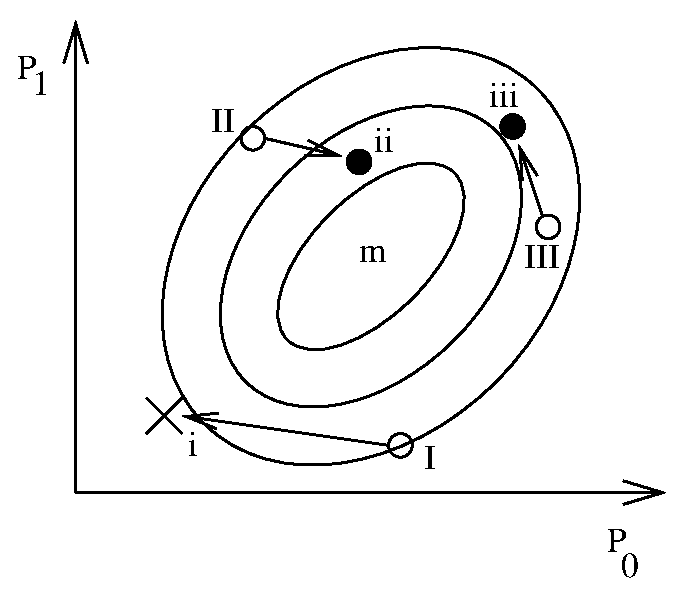
\includegraphics[angle=0,scale=0.65]{refine.evol.eps}
   \caption{Schematic sketch of an evolutionary algorithm.
    Two parameters P$_{0}$ and P$_{1}$ are refined in the search
    for the optimum solution. The ellipsoidal lines represent 
    lines of equal R-values. The global minimum is at point m.
    Members I, II, and III generate the new members i, ii, and iii
    by modification of the original parameter values.
    The new members ii and iii have an improved R-value, while
    member i has a worse R-value compared to the original member I.}
   \label{evo-evol}
\end{figure}

The algorithm begins by creating a group of parameter sets, see Fig.
\ref{evo-evol}. Each group 
member is a list of parameter values M:[$p_{0}, p_{1}, ..., p_{n}$],
and for each member the R-value or more generally speaking the
cost function is calculated. Within crystallographic applications, 
the R-value is usually calculated as described by Eq. \ref{diff-eq-rval}

Next, a new group of
parameter sets is generated. Several different algorithms for this
step exist. One possibility is to change each parameter by a Gaussian
distributed random number with mean zero, which is added to the original
parameter value. The variance of this distribution will vary from
parameter to parameter. The lattice constants, for example will
need another variance than the angles. In Fig. \ref{evo-evol}
the members I, II, and III create in turn the new members i, ii, and iii.
This modification  of a single parent member is comparable to the 
genetic mutation in biological systems. Most systems apply a second
modification, that mixes the parameter values of two different parent
members, a process that roughly resembles the sexual replication.

Once the new group of members has been generated, their R-values are 
calculated in turn. In the example child members ii, and iii have a
smaller R-value compared to their respective parent members, while
child i has a higher R-value than its parent. The next task to decide 
which members of the old parents and children shall be retained and 
form the next parent group from which the next children group is to be
generated. A number of different approaches exist for this task. One
option is to compare a child with its immediate parent and to keep the 
better of these two. In the situation depicted in Fig. \ref{evo-evol},
this would choose the parameter sets I, ii, and iii as parents for the
next generation. Another approach is to combine all parents and all
children into one group. From this group the N best are chosen as 
parents for the next generation. In Fig. \ref{evo-evol} this would
give the parameter sets ii, III, and iii as parents for the next 
generation, since these three sets have the three lowest R-values.

As the parameter values change from generation to generations, those
members survive that have better R-values. As consequence, the parameter
value evolve towards the minimum R-value. If the landscape of R-values
is more rugged compared to the simple situation of 
Fig. \ref{evo-evol}, one has to be careful not to refine into a
local minimum instead of the global minimum. The literature on 
evolutionary algorithms extensively deals with this issue.
%------------------------------------------------------------------------

\section{The differential evolutionary algorithm \label{diff-price}}

The essential feature of the differential evolutionary algorithm, 
introduced by Price and Storn \cite{prstla2005}, is the process, by which
new children are generated.

\begin{figure}[htbp]
   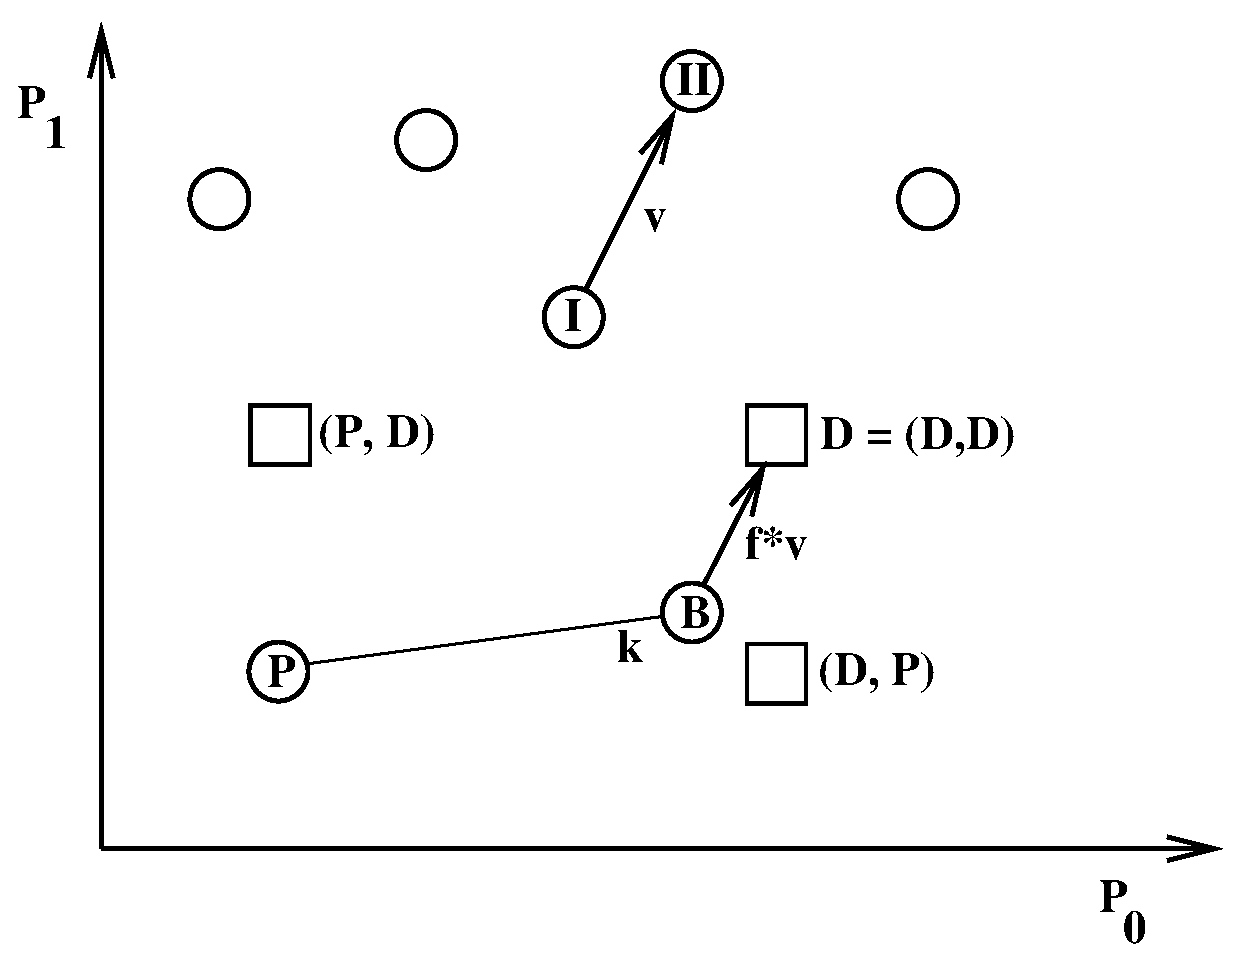
\includegraphics[angle=0,scale=0.45]{refine.diffev.eps}
   \caption{Schematic diagram of the differential evolution algorithm.}
   \label{evo-select}
\end{figure}

The algorithm picks in random sequence all members of the current 
generation, shown as circles in Fig. \ref{evo-select}. The current
parent has been marked by P in the figure. Another member, the base B 
is chosen at random. Next, two other members are also 
chosen at random, members I and II in Fig. \ref{evo-select}. The
differential evolutionary algorithm then calculates the difference vector
$\vec{v} ~=~ \vec{II} - \vec{I}$ between these two parents. This difference
is the part of the algorithm that coined the name. The difference vector
is multiplied by a factor f and added to the base member. 
All four members are different members of the population. The
scale factor f is a variable that is used to control the refinement
properties of the differential evolutionary algorithm. In general it
should be somewhat smaller than one. The sum of the base member and the
difference vector is a general point in parameter space, called the 
donor D. The donor D is the basic modification of th original parent
vector. In contrast to other evolutionary algorithms, there is no
direct connection between the parameter values of the parent P and its
modification, the donor D. 

After the determination of the donor D, the differential evolutionary
algorithm allows for a mixing of the parameter values between the 
parent P and the donor D. By random choice, parameter values are taken
either from the donor or from the parent. To ensure that the parent 
is not replicated, one parameter value is always taken from the 
donor D. The probability, by which the other parameters are taken from 
the donor D is called the cross over probability. Fig. 
\ref{evo-select} also illustrates the cross over process. If 
both parameters happen to be taken from the donor, the final child is the
donor itself. If parameter $p_{0}$ is taken from the donor and 
parameter $p_{1}$ taken from the parent, the child will be the position
labeled (D,P). Alternatively, if parameter $p_{0}$ is taken from the 
parent and parameter $p_{1}$ from the donor, the child will be the
position labeled (P,D). Thus the cross over leads to a mixing of 
the parameter values of the donor D and the parent P. It depends on the
refinement problem at hand, whether the cross over probability should 
favor parameters of the donor or the parent in order to ensure convergence. 

Once children have been created for all parents, their R-values are 
computed. The differential evolutionary algorithm compares the 
R-values of each parent and its immediate child. Whoever has the 
lower R-value survives and is treated as parent for the next generation.

Several modifications to this basic differential evolutionary
algorithm exist. The first modification concerns the choice of the
donor base B. In the standard algorithm, the donor base is chosen
randomly among the members of the population. As an alternative one
can decide to take the current best member as donor base for all
children. This will search predominantly in the neighborhood of the
current best member and thus speed up the convergence into the 
minimum close to the current best member. If, however, this minimum
is a local instead of the global minimum, chances are higher that 
all children will be within this local minimum as well.

Another alternative allows to add the scaled difference vector to
any point along a straight line between parent and donor base, the 
line marked k in Fig. \ref{evo-select}. A control variable 
{\em k} chooses the point. I the usual definition, the donor base 
is chosen if k=1 and the parent if k=0, and any point in between
for intermediate values of k. In principle k is not limited to 
the interval [0:1], and \Diffev does not limit your choice. 

Choosing the surviving members allows for another modification of the
original algorithm. Instead of a pairwise comparison of parent and
child, one can also group all M parents and all N children into one group.
Those M member of this combined group that have the lowest R-values
survive and are used as parents for the next generation. The status of
original parent or child is not taken into account. This approach will
usually lead to a faster convergence, albeit at the risk of convergence 
into a local minimum. If the number of children is increased 
beyond the number of parents, the 
{\em evolutionary pressure} increases and the convergence is generally
enhanced.

%------------------------------------------------------------------------

\section{Termination criteria \label{diff-term}}

Several different criteria may be used to terminate an evolutionary
refinement. 

\begin{itemize}
  \item {\bf Global minimum has been reached}\\
     If the values that correspond to the global minimum is
     known, the refinement can stop, once the lowest trial value falls
     within a defined threshold above this value. Unfortunately, in 
     case of structure refinements, the lowest R-value cannot be known
     before hand and this criterion is not well suited.
  \item {\bf Predefined number of refinement cycles}\\
     If the best R-value does not decrease for a given number of 
     generations, chances are that we are very close to the global minimum.
     Unfortunately, one can never know whether the refinement may not
     improve after just a another few generations. This criterion may, however,
     be used to determine a good refinement strategy. The main variables
     to the differential evolutionary algorithm are the population size, 
     the scale factor f by which the difference vector is multiplied, 
     and the cross over probability. If refinements with different 
     settings for these control parameters are allowed to run for a 
     given number of generations. Those control parameters that lead to
     the lowest R-values after these generations can then be taken as 
     good parameters for further refinement problems.
  \item {\bf Population statistics}\\
     For diffraction data, it is straightforward to calculate an expected
     R-value. The refinement can be stopped, once the best R-value 
     reaches this value, or at least comes close. Another choice could
     be to wait until all R-values have dropped to within a defined 
     range of R-values above the expected R-value. The corresponding
     parameter range may then be inspected to determine the corresponding 
     parameter uncertainties. If the model is insufficient, one may never
     reach this situation. Instead one could terminate the refinement
     once all R-values have become very similar to each other. If the
     lowest R-value is significantly above the R-expected one should 
     run the refinement again with different starting parameters, of 
     different control parameter settings to exclude convergence into a
     local minimum. If the parameters refine into the same minimum, the
     model should be analyzed and hopefully be improved.
  \item {\bf User intervention}
     The last choice is to run the refinement indefinitely and to 
     terminate the refinement manually be the user. Given the many 
     different disorder problems that \Diffev may face, this is the main
     termination criterion offered at present.

\end{itemize}

\section{Optimizing the performance \label{diff-opti}}

The examples in this section use the example from chapter
\ref{example}. Details given here are sketchy, refer to chapter
\ref{example} for full details.

Choosing the best setup for the refinement is in itself an abstract 
optimization task. One should choose those values for the control
parameters that will cause the refinement to find the global minimum
with the least amount of function calls. With regards to the
differential evolutionary algorithm one needs to select the best 
values for:

\begin{itemize}
  \item {\bf Population size}
  \item {\bf Scale factor f}
  \item {\bf Cross over probability}
  \item {\bf Choice of donor base}
  \item {\bf Selection mode} 
  \item {\bf Local search probability}
\end{itemize}

The actual values that give the best performance will depend on the
refinement problem at hand. See the discussion in chapters 2 and 
3 of \cite{prstla2005} for a further details. In the following we
show a few examples that illustrate how to find good parameter 
settings.

\subsection{Population size}

\begin{figure}[htbp]
   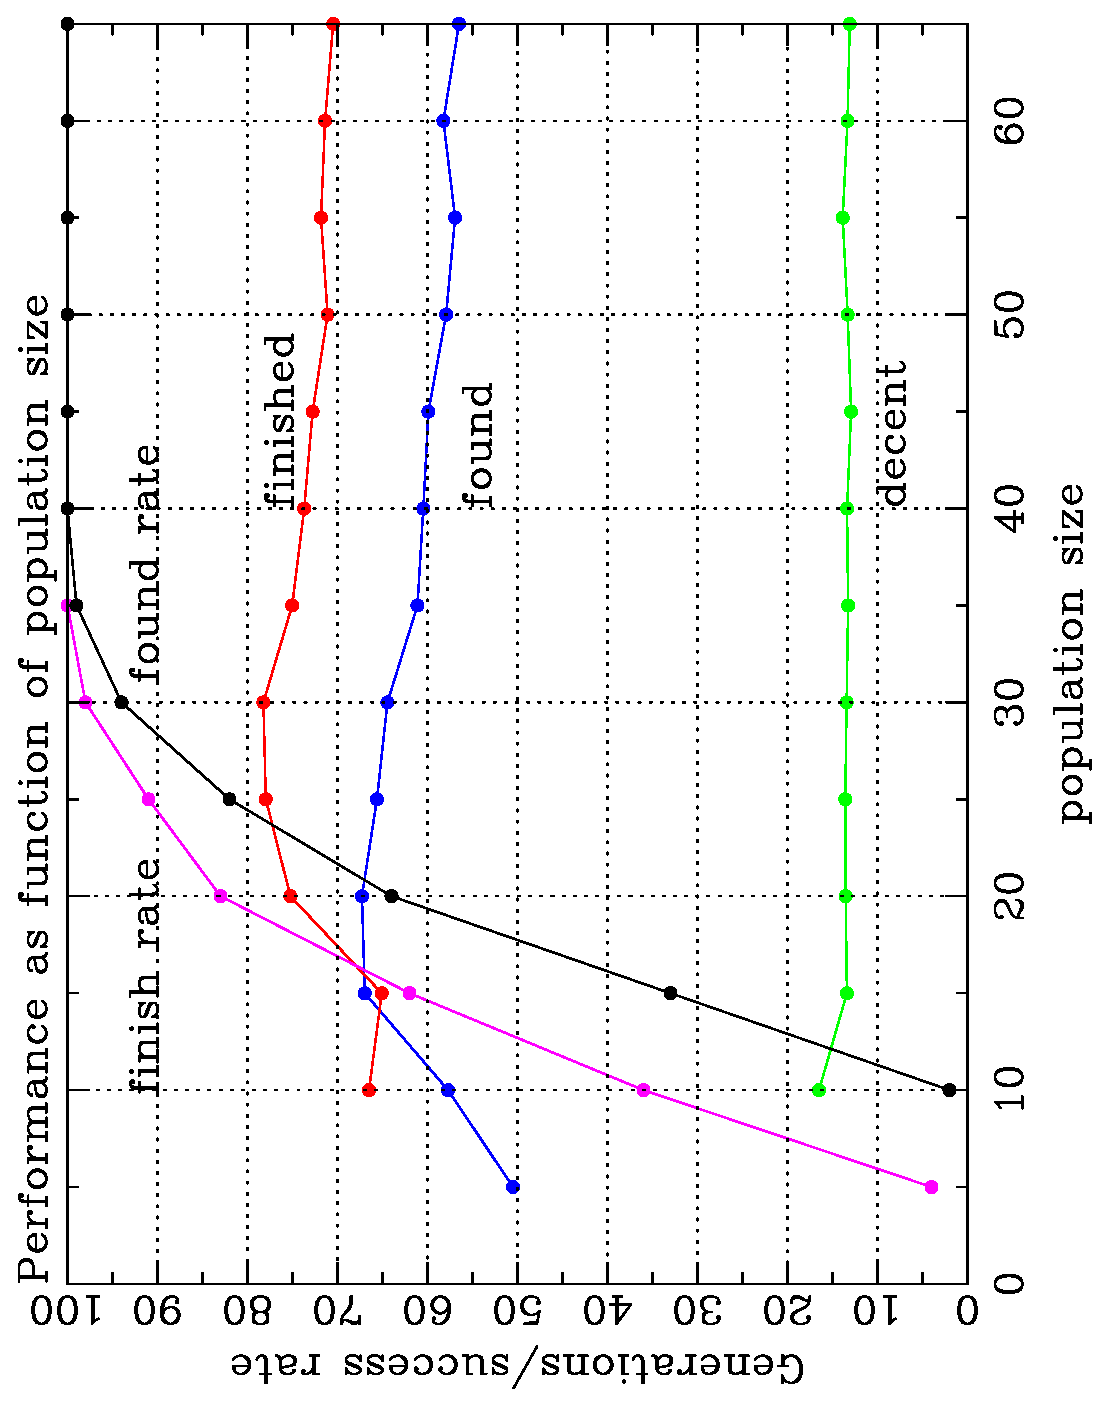
\includegraphics[angle=270,scale=0.45]{refine.pop.eps}
   \caption{Success rate as function of population size.}
   \label{evo-pop}
\end{figure}

If the population size is small, few permutations exist between the 
members of the population and there will be few locations that are
searched in the parameter space.

Fig. \ref{evo-pop} shows the effect the population size has on the
refinement of the modified arctan function. This function requires 
three parameters, and parameters 2 and 3 pose a challenge due to the 
high noise present in the data. The true parameters for the example
function were $P_{1}=100;~P_{2}=100.23;~P_{3}=0.1$. The refinement was run
for population sizes from 5 to 65 members. The donor base was chosen
at random, and the selection mode took the best members from 
the combined group of parents and children. The local search mode was 
switched off. The refinement was
considered successful, if the R-value fell below a given threshold. 
Due to the special function, this meant that the parameters are close
to the true parameters and that the refinement will from here on 
converge into the global minimum. The refinement was allowed to run
for 100 generations. Refinements that did not reach the global minimum
or did not finish to refine to the global minimum were considered 
failures. At each population size, the refinement
was repeated 100 times. Fig. \ref{evo-pop} shows the performance as
function of population size. The blue and red curves show the number 
of generations required to get close to the global minimum, respectively 
to finish refining into the global minimum. The black and purple curves
show the percentage of refinements that came close to the minimum, 
respectively finished refining into the global minimum within the 
allowed 100 generations. 

A population size of about 40 members is needed to ensure 
a 100\% success rate. At smaller population sizes, a larger fraction of
the refinements does not find the minimum and thus the refinement 
cannot be considered satisfactory. If the population size is increased
beyond 40, the number of generations required to get close to the 
minimum, respectively to finish refining into the global minimum 
decreases slightly. The increase in function calls due to the population
size increase is, however, higher than the gain obtained by faster 
refinements.

\subsection{Scale factor and cross over probability}

To test good values for these two parameters, the population size of 
40 was adapted according to the observations on the population size.
Both factors were chosen randomly in the interval [0:1]. As in the
previous investigation, the refinement was considered successful, if
the parameters reached the true values within 100 generations.

\begin{figure}[htbp]
   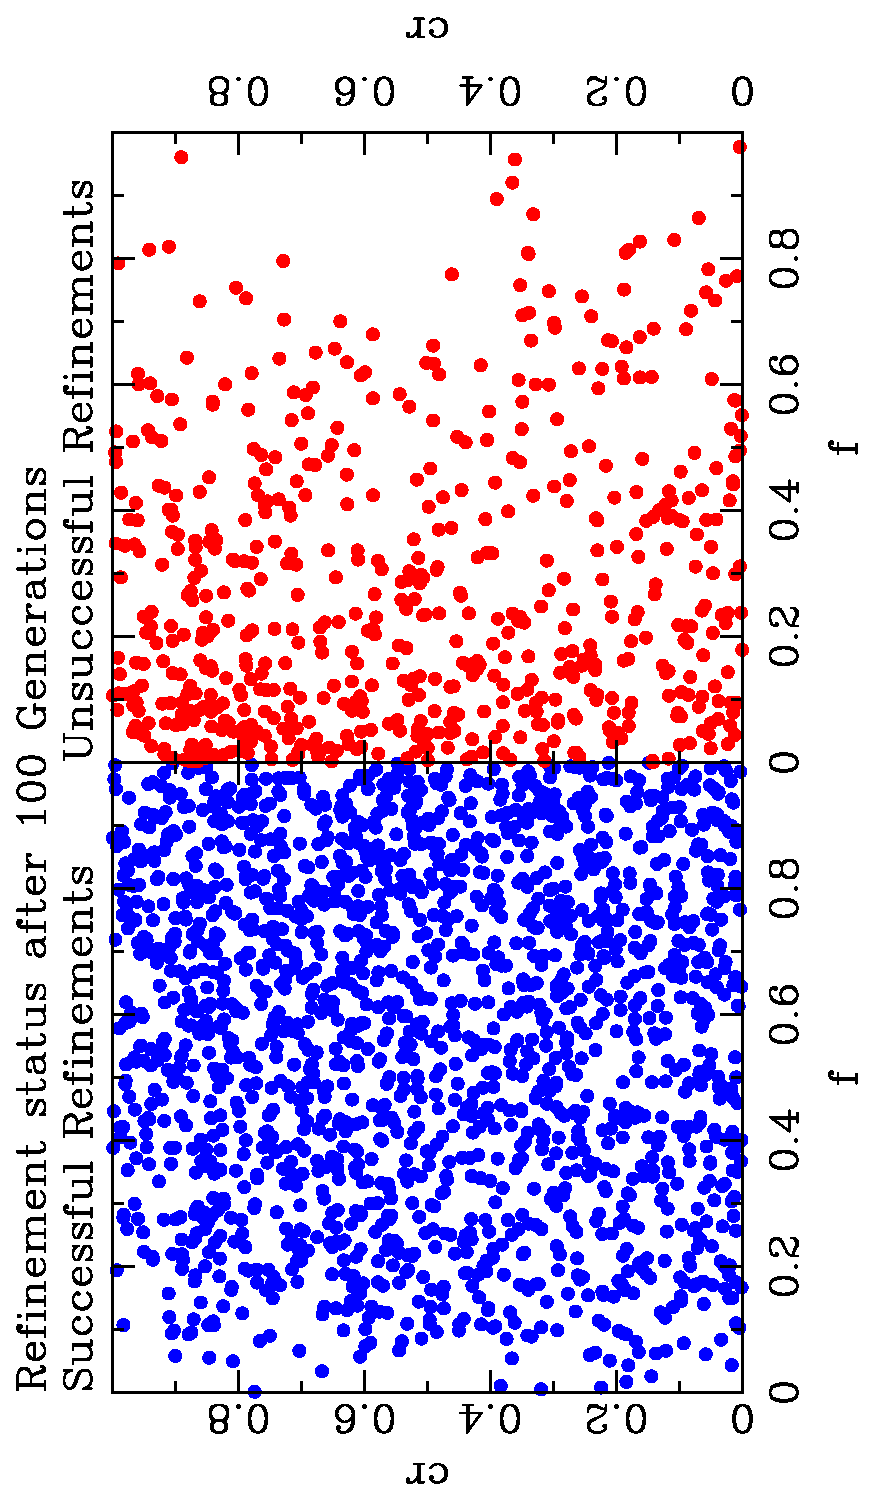
\includegraphics[angle=270,scale=0.55]{refine.fcr.eps}
   \caption{Success rate as function of scale factor f and
    cross over probability cr.}
   \label{evo-fcr}
\end{figure}

The figure shows that successful refinements of this example function
require a scale factor
that should be closer to 1. For very small scale factors, the 
algorithm effectively searches in the local environment of the 
donor base instead of a wide parameter range. In this example, this
increases the chance of refining into a local minimum.

\subsection{Local search probability}

A cut through R-value space along $P_{3}$ at $P_{1}$ and $P_{2}$ at their
respective optimum values shows a narrow minimum around the optimum
value of 0.1. This behavior might indicate that a local search around the
members might enhance the convergence into this narrow minimum. To
test this, two different test were performed, in which the local search 
probability was systematically varied from 0 to 1. 

For both tests with different local search options, otherwise identical 
control variables were used. The population size was set to 40 members,
the scale factor was 0.81 and the cross over probability 0.8. The donor
base was chosen randomly and the best members of the combined parent/children
group were selected. For each local search probability the refinement
was repeated 100 times.

Figure \ref{evo-lo} shows the number of generations required to 
find a parameter combination close to the global minimum (blue), the total
number of generations required to refine very close to the global minimum
(red), the number of generations required from the time the first 
parameter set is close to the global minimum until the global minimum is
reached (green), the percentage of refinements that came close to the 
minimum (black, and the percentage of refinements that finished refining
into the global minimum (purple).

\begin{figure}[htbp]
   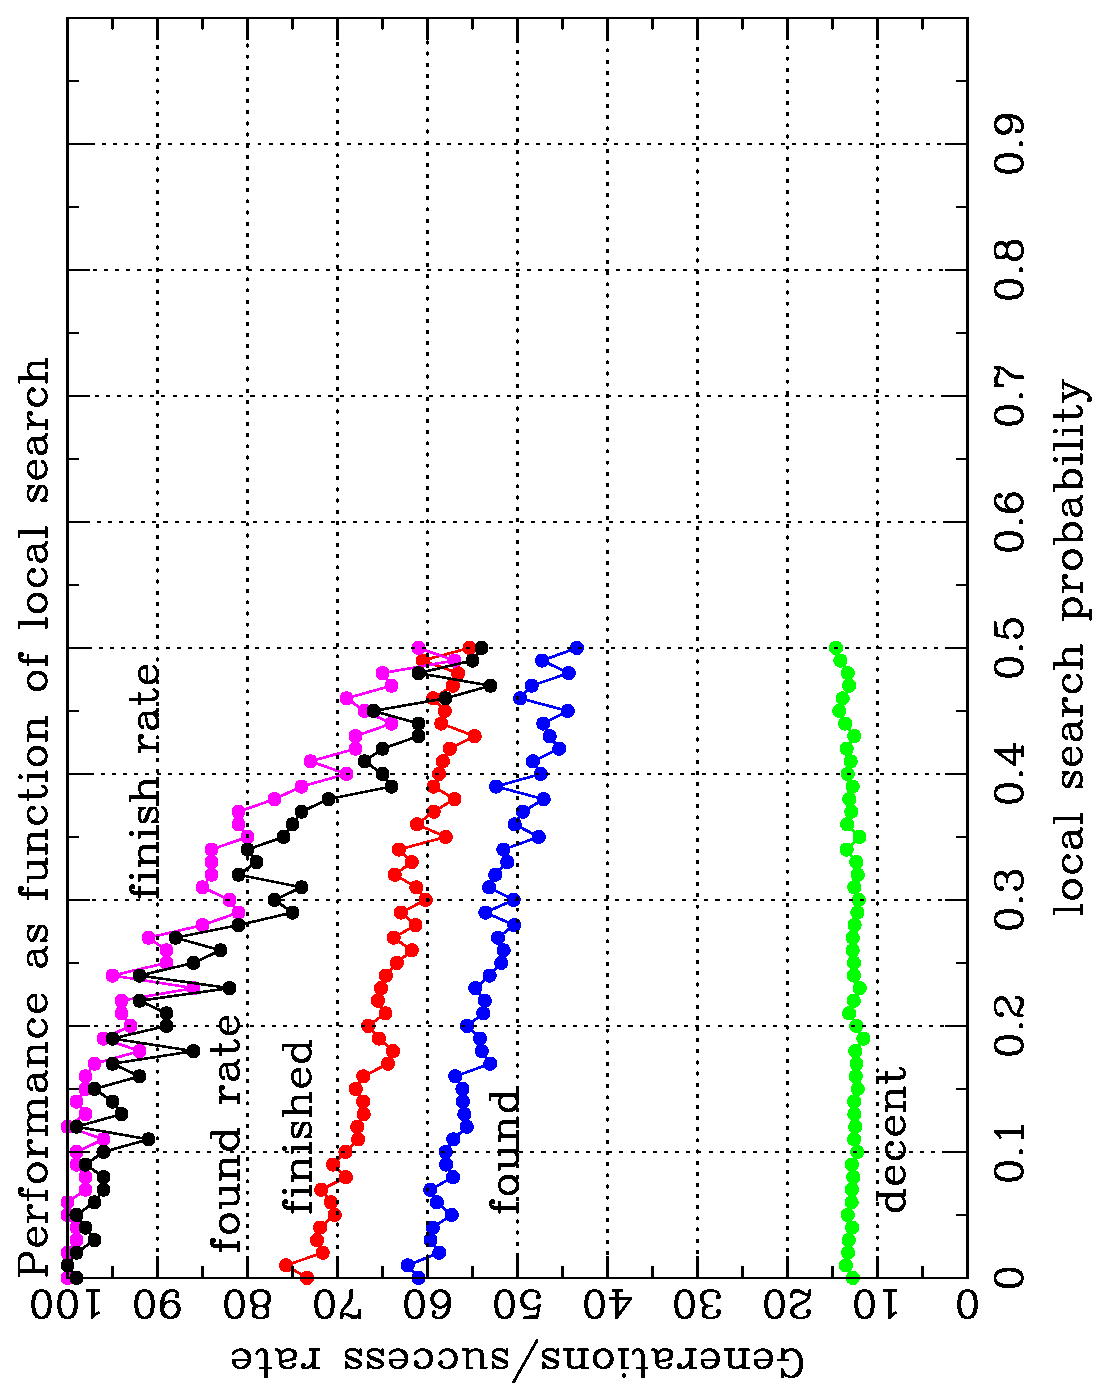
\includegraphics[angle=270,scale=0.34]{refine.lo.ada.eps}
   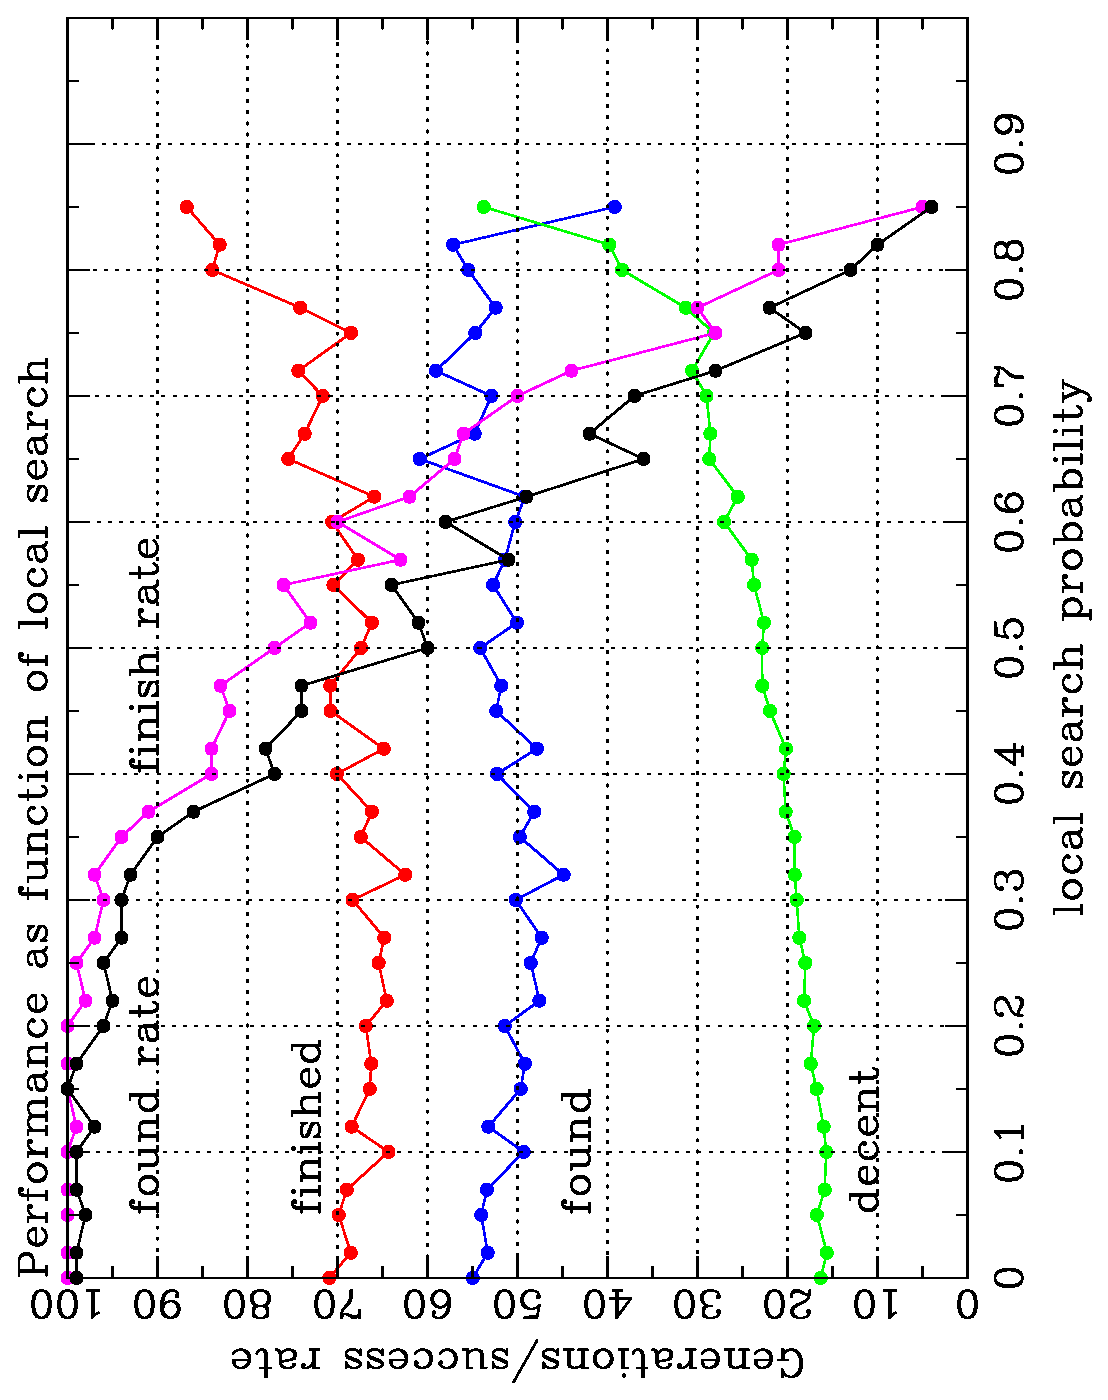
\includegraphics[angle=270,scale=0.34]{refine.lo.fix.eps}
   \caption{Refinement behavior as function of local search probability.
    Left, local search sigma adapted to 0.02 of the parameter spread,
    Right, local search sigma at fixed values (0.1; 0.1; 0.002). }
   \label{evo-lo}
\end{figure}

The refinement with adaptable local search sigma showed that the number
of generations required to find the global minimum decreases slightly
with increasing local search probability. Beyond a probability of roughly
15\%, the percentage of successful refinements starts to decline quickly.
For the refinements with fixed local search sigma, the effect on the
number of cycles is less pronounced. All in all one can see that the local 
search does not provide a clear effect on the refinement efficiency. 
In general, the original differential refinement algorithm seems to 
work better. 

\subsection{Limiting Parameters}

Sometimes it is advantageous to fix one or several parameters in order
to be able to perform a limited search. This is mostly helpful in the 
early stages of a refinement. Here one can refine a limited set of
parameters just to get a rough idea where the likely global minimum is
located. If parameters are not correlated one can limit the refinement
to a small subset or even to a single parameter. The optimized value
for this parameter should be reasonably close to the global minimum, 
if the parameter is that is refined is not correlated to the other
parameters. The main advantage of such a search is that the dimension of
the search space is much smaller and thus a much smaller population size 
will be sufficient.

To {\tt fix} and to {\tt unfix} a parameter, \Diffev offers the two
commands {\tt fix} and {\tt release} with the respective syntax:

\begin{MacVerbatim}
fix P_lata, best
fix P_latx, 5.00
\end{MacVerbatim}

With the second parameter set to {\tt best}, the parameter is set to the 
value of the member with the current lowest cost function, i.e. R-value.
Alternatively you can set the parameter to another value, with the limitation
that the parameter must be within the absolute boundaries for this 
parameter that were set with the {\tt newpara} command or by assigning a
value to the variables {\tt pop\_xmin[]} and {\tt pop\_xmax[]}.

For all subsequent cycles, the value of this parameter will be fixed to
the chosen value. As this will change the parameter combination of all
but the best member, the respective R-values for the next refinement 
cycle are invalidated to ensure correct testing of the next generation 
with respect to the generation prioor to the {\tt fix} command.

The complementary {\tt release} command allows you to set a new range of
trial parameters for this parameter:

\begin{MacVerbatim}
release P_lata, range:sigma
release P_latc, range:sigma, value:set_point, min:par_min, max:par_max
\end{MacVerbatim}

In the simplest form, the parameter is initialized again within a 
window of +-sigma around the value of the current best member. 

The absolute window for this parameter is set to a range of +-3*sigma
around the value of the current best member.

This new absoute window might be too wide or may include parameter 
values outside a physically sensible limit. As an example, a 
atomic displacement parameter may end up with a negative lower 
boundary. To prevent this behavior, the optional parameters
{\tt min:par\_min} and {\tt max:par\_max} allow yo to fix the 
absolute boundaries to proper values. 

The optional parameter {\tt value:set\_point} allows you to center
the initialization window at a value {\tt set\_point} instead
of the automatic centering around the current best value.


\section{Invoking the slave program \label{diff-invoke}}

The typical refinement requires the following steps:

\begin{itemize}
 \item definition of the problem
 \item initialization 
 \item A loop over the required generations
within each loop the simulation of all crystal structures and the calculation 
of all cost functions / R-Values
 \item A comparison of old and new cost function values / R-values and generation
of new trial parameters.
\end{itemize}

In the first step the number of population members and the number of refine-able
parameters and their allowed range must be specified. \Diffev furthermore 
expects the definition of log files to keep track of the refinement. See the
examples in \ref{example} for details on the commands.

The initialization step will assign starting values to all parameters that you
want to refine. \Diffev expects you to provide for each parameter a range 
within which the parameters are allowed, and a (narrower ) range for the 
starting distribution. The initialization will place the starting parameter 
values with an even random distribution with the starting window. See
\ref{example} for further details. 

As of version  5.3.0 the trial parameters need not be written to a file on
the disk. If \Diffev is used within the \suite, the trial parameters
can be transferred directly to the slave program via the command:
'init silent'.

Within the loop the slave program that will simulate the crystal and evaluate
the cost function / R-Value must be started. As of version 5.4.0 a unified
command 'run\_mpi' should be used for this purpose. The command will 
recognize whether \Diffev runs as stand alone program or as part of the
discus\_suite (the strongly recommended style) and if the program uses MPI to 
process the slave program in parallel. An identical macro for the slave 
program can be used in all cases. 

The slave program is actually started 
by \Diffev as:
\begin{MacVerbatim}
discus -macro discus_main.mac PWD kid indiv > discus_log.xxxx.yyyy
\end{MacVerbatim}

If \Diffev is part of the \suite, the suite will internally switch to
the discus section to execute the macro 'discus\_main.mac'. If \Diffev is
run as a stand alone program (highly discouraged), it uses a system 
call to start the \Discus 
program with the command line option to execute the macro. In both cases
identical \Discus macros can be used. The one exception is the 'silent'
option for the 'init' and 'compare' commands. This option is available
within the \Suite only. For the stand alone version of \Diffev no direct
communication exists between \Diffev and \discus. The trial parameters and
the R-values need to be written to disk to communicate between the 
programs. It is strongly recommended to use the \suite.

\subsection{Parallel Refinement via evolutionary algorithms \label{diff-parallel}}

As the refinement in DIFFEV is based on a large population, it 
naturally lends itself to parallel performance. This version of DIFFEV has a 
build in support for a MPI based parallel distribution. Within this model,
each of the children is simulated / calculated in parallel to each other. 
On a large scale computing facility you will typically submit your job to 
a queue and you will have to request a specific number of nodes and over all
wall time. As example we will use the queue system at the high performance
center in Erlangen. Take this as a general guide and refer to your system
for changes that you might have to do.


Within this general set up the simulations of all crystal structures can be 
performed independently and thus in parallel. If the calculation of the 
r-value takes considerable time this can be performed in parallel as well. 
This parallel calculation must only be carried out once the simulation
is finished.

If the simulation involves small crystal structures, or a distribution of
defects and/or sizes, you might need to simulate several individual 
structures for each member of the population. Again these simulations can be
performed in parallel.

MPI is a widely distributed system to run jobs in parallel. You can even 
use it effectively on a multi core computer. To use DIFFEV with MPI you need 
to turn on the MPI option during compilation or run the MPI version from
the \Discus download server.

A set of command to run the refinement in parallel will be like:

\begin{MacVerbatim}
   set prompt, redirect
   @diffev_setup.mac       ! all the set up commands 
   init silent             ! Initialize the population
   do i[0]=1,10            ! Make a loop over 10 refinement cycles
      run_mpi discus, discus_main.mac, repeat:20, compute:parallel, logfile:discus_log
      run_mpi kuplot, kuplot_main.mac, repeat:20, compute:serial,   logfile:kuplot_log
      compare
   enddo
   exit
\end{MacVerbatim}
 
The {\tt run\_mpi} command instructs DIFFEV to run the program specified as
first parameter in parallel. The second parameter is the macro that the slave 
program will execute. 

Starting with version 5.17.0 the remaining parameters take on the form for
optional commands. Backward compatibility holds.

The parameter {\tt repeat:} tells the slave section how often a calculation for 
an member has to be repeated. Such a repetition is often necessary if you simulate
small crystals with defects that are distributed with any kind of randomness. In
these cases an individual crystal is not a good representative of the many 
possible defect distributions. You will get a reliable result only if the simulation
is repeated and the corresponding data /diffraction /PDF/...) are averaged.

The parameter {\tt compute:} tells the slave section whether it should calculate
these individual repetitions serially within a single macro or whether the 
individual simulations will be calculated in parallel alongside the parallel
distribution of all the members.

The parameter {\tt logfile:} enables you to save the output from the slave 
section into a log file. This will be helpful during the development of your
refinement. Once everything works fine, omit this parameter or set its 
value to {\tt none} or to{\tt /dev/null} to discard the output. The
log file parameter will be augmented by a four digit number with leading zeros 
for each member. If the individual repetitions are done in parallel, the 
filename is augmented by a further four digit number that stands for the 
current individual repetition.


The slave section is started by DIFFEV as:
\begin{MacVerbatim}
discus -macro discus_main.mac > discus_log.xxxx.yyyy
\end{MacVerbatim}

The refinement parameters, the child number and the individual repetition
number are transferred internally and can be accessed with the macro
{\tt discus\_main.mac}. 
The log file
name is extended by two four digit numbers xxxx and yyyy, which hold the 
values of the child and the individual repetition.

\Diffev uses several variables with fixed name that are transferred to the 
slave section. These are:
\begin{itemize}
  \item REF\_GENERATION  The current refinement generation number
  \item REF\_MEMBER  The population size
  \item REF\_CHILDREN The number of children for which the simulation is carried out.
  \item REF\_DIMENSION The number of parameters to be refined
  \item REF\_KID The current child number
  \item REF\_INDIV The individual repetition number.
  \item REF\_NINDIV The total number of individual repetitions that are needed.
  \item INDI\_PARALLEL Is the calculation of the individual repetitions carried out
              serially by the macro {\tt discus\_main.mac} or distributed in parallel.
\end{itemize}

Within \Diffev the parameters to be refined are set by the command {\tt newpara}.
The name that you give to the parameter on this command is stored as a user 
defined variable and given its proper current value. Use this variable name within
the macro {\tt discus\_main.mac} as well. See the second example in\ref{example}
for further details.

The number of parallel instances that will run depends on your MPI system. 
On a stand alone computer with several cores you will start \Diffev as 

\begin{MacVerbatim}
   mpiexec -n 8 discus_suite -macro refine_main.mac
\end{MacVerbatim}

For the \Suite, the main refinement macro should switch to the \Diffev
section to the refinement and return to the \Suite as in: 

\begin{MacVerbatim}
diffev
... setup
... init silent
... loop over generations
exit   ! This goes back to the SUITE
exit   ! This will finish the SUITE
\end{MacVerbatim}


In this example, MPI will reserve 8 cores for your job, execute \Diffev 
as a section of the \Suite, which 
must be located in a directory where the standard PATH environment variable will 
find it. The macro {\tt refine\_main.mac} must contain all instructions 
for DIFFEV, including the {\tt set prompt, redirect} and final {\tt exit} 
commands.

The MPI scheduler does not know how long a calculation by the slave program
may take. This might cause an idle state for some or almost all CPU's once 
almost all children in a given generation have finished. This will cause 
your system not to run as efficiently as possible. Some of this idle state
cannot be avoided. You can reduce the idle state if you keep the number of 
requested CPU's much smaller than the number of simulations required for
one generation. Under these settings, each CPU will have to run several 
simulations and you can hope that the work load will average out. To average
the calculations DIFFEV sends the CHILDREN times NINDIV calculations in
a double loop. The inner, faster index is over all CHILDREN, the slower over 
all individual calculations.

As of version 5.17.0 the \Diffev section has been optimized, see the 
section \ref{diff-parallel-c} in this chapter.

\subsection{Computational aspects of parallel refinement \label{diff-parallel-c}}

In this section we will cover some computational aspects of the refinement
that may guide you to optimize the performance. Fig \ref{fevo-over} shows a
schematic overview of the parallel refinement. When you start the \Suite
via mpi as in

\begin{figure}
   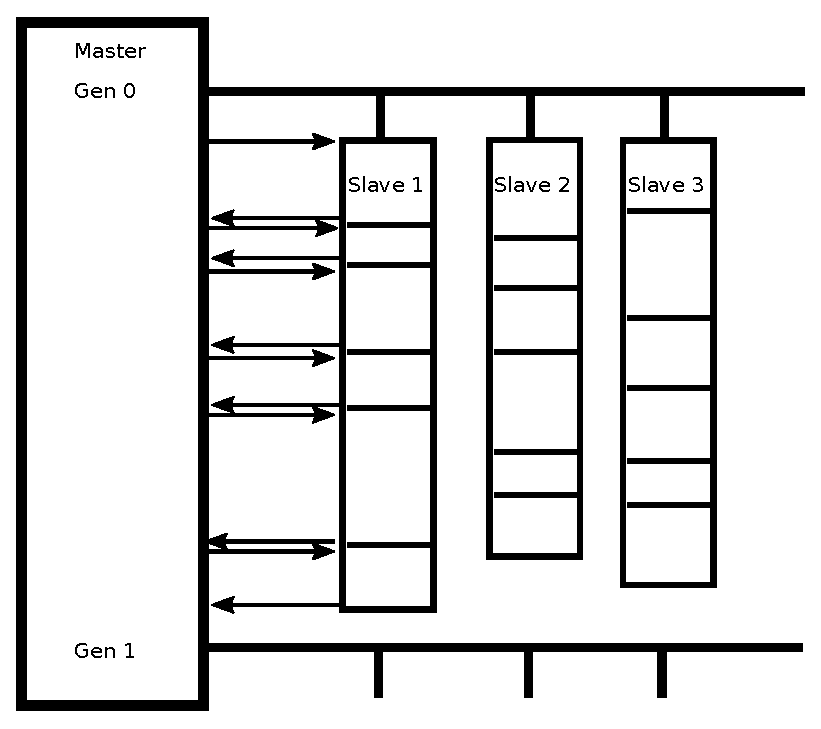
\includegraphics[angle=0,scale=0.65]{Master_slave.eps}
   \caption{Overview of parallel refinement process }
   \label{fevo-over}
\end{figure}

\begin{MacVerbatim}
   mpiexec -np 8 diffev -macro refinement.mac
\end{MacVerbatim}

the \Suite starts a master process that will in turn start np-1 slave 
processes. In each generation the master process will instruct the slaves
to perform several tasks. Lets say you you have a large population and
each individual simulation does not have to be repeated. The master will 
then instruct the slaves to start the calculation for the first np-1
members. As soon as a slave is finished, it will send back the result to 
the master and receive the instructions to start the calculations for
the next member. This communication is indicated by the arrows between the
 master and the first slave in Fig \ref{fevo-over}. In many cases the 
calculation times for each member will differ as indicated by the 
different vertical positions of the horizontal bars within each slave.
Ideally all slaves would terminate their last calculation at the same time. 
This would minimize idle time on the computer. This is, however,
difficult to enforce and some idle time for almost all slave can hardly be
avoided. 

If the computation time for all members is identical, the number of slaves
and the population size should be matched such that the population size is
an integer multiple of the number of slaves np-1. This will ensure that
all slaves will perform calculations for an identical number of members and
will be finished at the same time. If the population size is larger by
one member, a single slave will be busy with this last member while all
other slaves are just waiting for new instructions.

If the computation times for the different members differ but can be estimated 
ahead of times it is best to start to distribute the large jobs first and then
once these are done to hand out the shorter jobs. Those slaves that receive
the shorter jobs will perform calculations for more members that those 
slaves that receive the larger jobs. If the large jobs are handed out first, 
the chances are optimized that all the shorter jobs will finish roughly at the 
same time.

If the computation times cannot be estimated ahead of times, some idle time
is likely to occur. To reduce the amount of idle times each slave should perform
calculations for several members. As in the last paragraph, those slaves that
happen to receive larger jobs will perform calculations for fewer members. 
With several jobs per slave the fluctuations at the end should be about
half the computation time for an individual average job. 
If, as the other extreme, each slave were to 
calculate just one simulation, the one slave that takes the longest
calculation will force all other slaves to be idle until it is finished.
This will cause a huge amount of idle time.

At the moment the \Suite does not attempt to estimate how long
each calculation will take. There are just too many different parameters
that will influence the time like nanoparticle size, number of atoms, number
of atom types, time spend within a Monte-Carlo simulation etc. Given this
lack of information the idle time is minimized if each slave performs 
several calculations.  

The situation is slightly different if the calculations require the need 
to perform each simulation several times for a given member. This will be 
the case for example if you simulate small nanoparticles and the simulation
involves the creation of (randomly distributed) defects. As the individual
nanoparticle is small, its structure and as a consequence its powder 
diffraction pattern or PDF will not be a good representative of all possible 
structural conformations. You will have to repeat the simulation again for the 
same set of parameters. Afterwards all the individual powder pattern /PDF's
will have to be averaged. If an individual member has to be repeated N times,
the total number of simulations will of course be N times as large. To reduce 
the idle time the \Suite will hand out jobs for the first individual calculation
for each member first. Once all these are done the next individual calculations
will follow. All individual repetitions for an individual member likely
require a similar amount of time, while the requirements for different members 
may vary.

Once all members and all individual repetitions have been performed the \Suite
will have to average the temporary results. This averaging process can of 
course be performed in parallel as well. This raises two further issues 
related to the architecture of the computer at hand. 

A local computer or local compute server has an architecture similar to 
Fig. \ref{fevo-arch}. Several 
CPUs or cores perform the computing and MPI can distribute the workload onto 
these CPUs or cores. The CPUs share a common disk to store permanent data. 
At a large scale compute facility many of these units are combined. The local 
storage at each of these nodes often is a solid state memory instead of a 
traditional hard disk. A very large central disk provides storage space for 
global results. The scheduling process at such a high performance compute
center (HPC) typically give your job a privileged and sole access to all CPUs at 
a node and you process may request several nodes at the same time. The 
communication between the CPU's on a node and their local 
disk is fast, efficient and only interferes with you own jobs. The communication
to the central hard disk is common to all processes by all users at the HPC. 
Thus this communication should be reduced as much as possible as it may slow 
down your own process and that of other users as well. 

\begin{figure}
   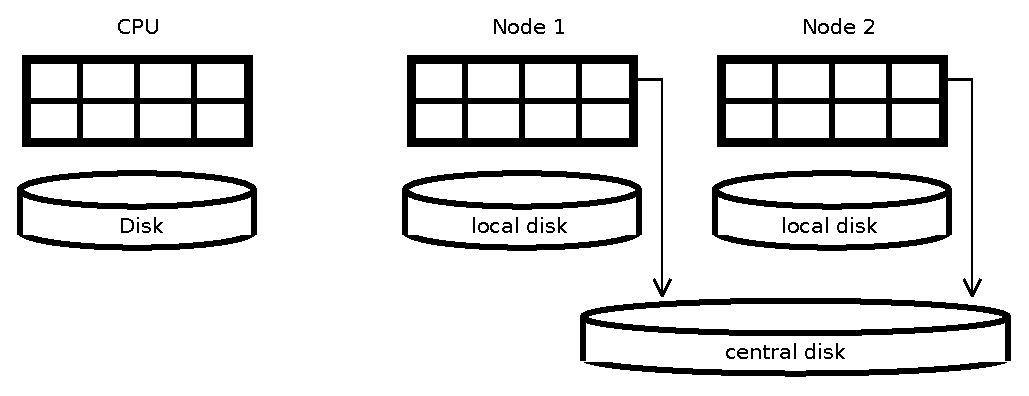
\includegraphics[angle=0,scale=0.65]{arch.eps}
   \caption{Simplified architecture of single PC with eight core CPU, left,
            and multi node HPC, right}
   \label{fevo-arch}
\end{figure}

The MPI distribution usually does not offer a direct assignment of a 
particular job to a specific core. This means, that the master process 
usually has no means to predict on which CPU a given calculation will occur. 

As of version 5.17.0 and later ones, the \Diffev section tries to optimize
the internal distribution of jobs onto the available nodes and their individual
cores as best as possible for any compute environment.

Keep in mind that we can have two different refinement situations:
\begin{itemize}
  \item The calculation for a member does not have to be repeated several 
        times
  \item The calculation for a member does have to be repeated several 
        times and the results need to be averaged once all calculations
        have been performed
\end{itemize}

Independent of this you may have two different compute architectures
available for your refinement:
\begin{itemize}
  \item A local PC or local small scale server with a single node
  \item A HPC center with many nodes, each node has its own local 
        storages common to all cores on this node
\end{itemize}

To match your refinement situation to the local architecture and to optimize
the performance \Diffev offers two different refinement styles:

\begin{MacVerbatim}
variable integer, nindiv
REF_NINDIV = 20
... diffev setup ...
pop_n[0] = 192
pop_c[0] = 192
... further diffev setup ...
... FIRST style
run_mpi discus, dis.diffev.mac, repeat:REF_NINDIV, compute:serial, logfile:/dev/null
...
... SECOND style
run_mpi discus, dis.diffev.mac, repeat:REF_NINDIV, compute:parallel, logfile:/dev/null
run_mpi kuplot, kup.diffev.mac, repeat:REF_NINDIV, compute:serial, logfile:/dev/null
\end{MacVerbatim}

Within the first style \Diffev will start pop\_c calculations. here in this
example arbitrarily set to 192. These 192 calculations will be distributed in
parallel onto the available CPUs. If the model requires any repetitions, the
\Discus macro here {\tt dis.diffev.mac} will have to include a loop over these
repetitions. The \Discus macro also needs to include a {\tt branch} to the 
\Kuplot section to calculate the R-value. As all repetitions for a given member 
are performed serially on a single CPU, you can write the \Discus output
data either onto a hard disk or directly into the \Kuplot memory space. The 
latter is done by prepending the output file name by the string {\tt kuplot}.
See the \Discus manual for further details. As the individual calculations 
during the refinement are temporary data of no long term relevance, it is a
good idea to avoid disk input/output. Thus the internal write is recommended.

Within the second style \Diffev will start pop\_c times nindiv calculations.
In this example this results in a total of 3840 calculations that can all be
performed in parallel. Each time the \Discus macro {\tt dis.diffev.mac} will
calculate data for just one member and will have to write these data onto a 
disk. Once all 3820 calculations are finished, \Diffev will instruct \Kuplot 
in a second parallel job to average all calculations for a given member and to 
calculate the corresponding R-value. As a single \Kuplot slave needs to average 
all repetitions, the parameter {\tt "compute"} is set to {\tt "serial"}. 
In this second model you need to write 
the data onto a disk, as the memory requirements would be too large for 
internal storage. A more stringent reason to write the data onto disk is that 
a single slave will perform calculations for members and individual repetions
in an unpredictable sequence. One can expect that the calculations for one 
member are performed by different slaves.

Now lets have a look at strategies to run these two different schemes on the 
two compute architectures. Common to both architectures, you will have np-1
processors available to perform actual calculations while the one master
processor keeps itself busy with administrative tasks. All slave processors 
should perform several jobs as this minimizes the risk of a long idle time 
at the end of a generation. 

\begin{itemize}
  \item Single PC or small server \newline
        On these systems several users might be active or you may run several 
        refinements or other tasks. As these tasks can take up idle time the
        following rules can be relaxed.
      \begin{itemize}
          \item No individual repetitions. The number of members should be
                an integer multiple of (np-1). To reduce the idle time the
                multiple should be high. 
          \item With repetitions. Both computation models are an option. If
                the calculation times are long per repetition you will not
                do too many disk I/Os to slow you down or to risk the integrity
                of your hardware. If the calculation time is fairly short, it
                might be kinder to your hardware to choose th first computational 
                model as temporary data can (and should) be saved internally.
      \end{itemize}
   \item High Performance Compute center \newline
         On these systems you will have sole access to a given node and its CPU.
         Local disk I/O is fast and does not cause wear and tear if the storage
         is a solid state disk. As you are the sole user, idle time should be
         minimized. A lot of disk I/O across the network onto the central disk
         will be frowned upon and should be reduced as much as possible.
      \begin{itemize}
          \item No individual repetitions. The number of members should be
                an integer multiple of (np-1). To reduce the idle time the
                multiple should be high. As a single node often has 24 or more
                CPUs request few nodes and long wall time instead.
          \item With repetitions. Both computation models are an option. The 
                second model makes better use of the many processors available.
                As of version 5.17.0 \Diffev will place all individual repetitions
                for one member onto the same node. If the local storage at a node 
                is a solid state disk the temporary storage will not significantly 
                slow down your process. Thus different slave processes that run on 
                the same node can calculate individual repetitions for any of the
                members on that node. The number of members should still be 
                an integer multiple of (np-1) but the factor can be reduced. The
                (large) number of individual repetitions will level out the workload
                at each core of a given node.
      \end{itemize}
\end{itemize}
%------------------------------------------------------------------------

%------------------------------------------------------------------------
% Chapter:  Introduction
%------------------------------------------------------------------------

\chapter{Example refinements \label{example}}

The example in this chapter will be used to explain in detail the 
commands and control variables that \Diffev uses. The example is a 
simple function y = F(x). While this restriction eases the display of the 
data, and refinement process, it does not impose a restriction on the
settings.

The macros and input data needed to run this example are found along
with the \Diffev source code, in the directory {\em diffev/TESTS}.

\section{Nanoparticle refinement}

In this section  a full blown refinement of a disordered nanoparticle 
structure is illustrated, which is also to be found in the DISCUS 
book, \cite{nedpro}. The data for the nanoparticle are taken from
\cite{neder2007}. The nanoparticle sample consists of ZnSe nanoparticles.
The PDF was derived from X-ray powder diffraction data taken at beam line 
BW5 at the former storage ring DORIS at DESY, Germany. 

\begin{figure}
   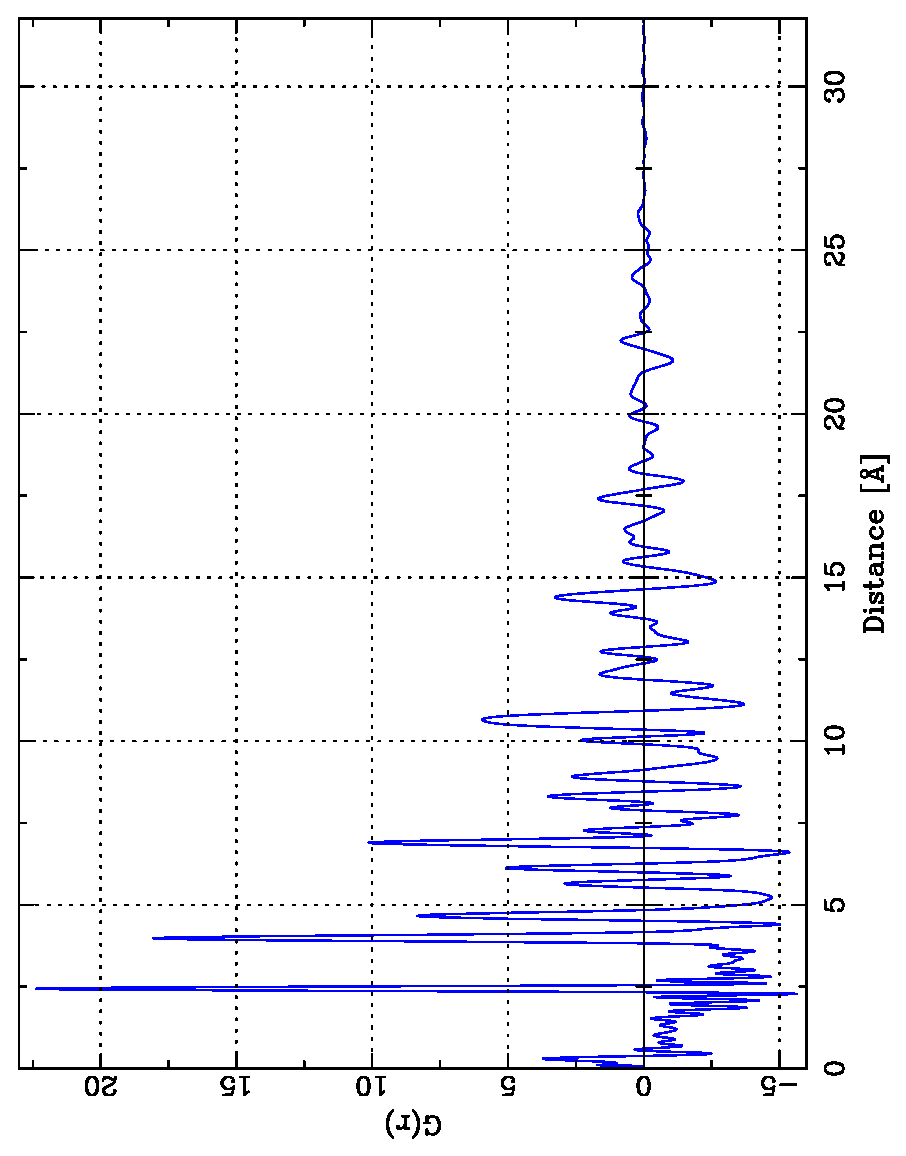
\includegraphics[angle=270,scale=0.45]{znse_grexp.eps}
   \caption{Experimental PDF for ZnSe nanoparticles}
   \label{fexa-znse-grexp}
\end{figure}

The experimental PDF suggests nanoparticles with diameter around 3 to 4 nm.
As bulk ZnSe crystallizes in the Zincblende structure, this provides for
a good starting model. Further modifications include an ellipsoidal shape
rather than a spherical shape and the inclusion of stacking faults that
allow for an alternation of locally cubic and hexagonal sequences. 
The first interatomic distances are observed at 2.44\AA{} and at
3.98\AA{} only. These two distances impose a locally tetrahedral environment,
and the stacking faults have to preserve this environment. TEM images
indicated that lattice fringes across the particles appeared undisturbed.
This is consistent with a model in which one of the symmetrically
equivalent cubic [111] directions is along the long axis of the ellipsoids.
Stacking faults will shift the layers normal to this direction and 
apparently no stacking faults are present along any of the other [111]
directions. 

As the nanoparticles are small, an individual simulated particle that 
contains stacking faults will not be a good representation of all 
possible configurations. See \cite{nedpro} for a full discussion. In the
refinement we will thus have to calculate individual nanoparticles 
several times for each set of parameters and average the corresponding 
calculated PDFs.

The main refinement macro consists of the following steps, which are shortly
outline before we go into the full details:
\begin{MacVerbatim}
diffev                        ! Switch to diffev section
#
  @cleanup.mac                ! Remove old files
#
  @setup.mac                  ! Define number of individual repetitions
  @get_model.mac              ! Define the refinement model to use
  @diffev_setup.mac           ! Define refinement details
#
  init silent                 ! initialize all parameters, silently no files are written
#                             ! The command can be omitted 
#
  do i[0]=1, 200              ! Number of refinement cycles 
    echo "Loop GENERATION %4d %4d", i[0], REF_GENERATION
    !                         ! Run discus section with macro dis.diffev.mac, no repetitions
    run_mpi discus, dis.diffev.mac, repeat:REF_NINDIV, compute:serial, logfile:LOGFILES/d
    compare silent            ! Compare R-values to previous generation
  enddo
exit                          ! Back to suite
exit                          ! Finish the suite as well
\end{MacVerbatim}
With the first line the \Suite is  instructed to switch to the \Diffev section. 
The {\tt cleanup.mac} macro contains line to remove all files from a previous
refinement run. The commands work on all operating systems and do not ask to
confirm the removal of the files. Next macro {\tt setup.mac} defines the number 
of individual repetitions that need to be performed for each parameter set i.e. 
for each member of the population.  the macro is short, and essentially consists
of the one line:
\begin{MacVerbatim}
REF_NINDIV = 20
\end{MacVerbatim}
If you look at the remainder of the main macro, you'll notice that 
corresponds to the parameter for the optional {\tt repeat:} on 
the {\tt run\_mpi} line.
You can run the individual repetitions either serially in {\tt dis.diffev.mac}
with {\tt compute:serial} or
run parallel versions of this macro. 
These models are explained 
further down after this quick overview. 

For this example, the user can
specify four different nanoparticle types:
\begin{itemize}
  \item a spherical particle with no stacking faults
  \item a spherical particle with stacking faults
  \item an ellipsoidal particle with no stacking faults
  \item an ellipsoidal particle with stacking faults
\end{itemize}
Macro {\tt get\_model.mac} reads the users choice. If the user had chosen 
a particle with no stacking faults, there will be no need to average
several individual particles. Accordingly, the choice in {\tt setup.mac} is
overwritten by setting the value of {\tt REF\_NINDIV} to one.
Next, macro {\tt diffev\_setup.mac} does all the detailed setup for the 
refinement. Once the setup is done, {\tt init silent} initializes the first
generation. As of version 5.16 this command can actually be omitted, as 
\Diffev recognizes the state it is in and will perform an initialization
if needed.

In the following loop over a fixed number of refinement cycles 
\Diffev uses the \Discus section to simulate the nanoparticles and to calculate
the agreement between the experimental and calculated PDFs. The {\tt compare}
command instructs \Diffev to compare the current generation to it parents and
to create a next generation of trial parameters.  
The final two lines finish the \Diffev section and the \Suite program itself.

On a Unix type operating system the \Suite program will be started with a line like:

\begin{MacVerbatim}
mpiexec -np 250 discus_suite -macro refine.mac
\end{MacVerbatim}
Alternatively you can usually use {\tt mpirun} and most MPI environments 
will take either {\tt np} ( the proper form ) or {\tt n} to specify the 
number of parallel processes to be started. 

With Windows start a first \Suite window and at the command prompt type:

\begin{MacVerbatim}
parallel refine.mac
\end{MacVerbatim}

An optional parameter allows control over the number of parallel processes as 
well:
\begin{MacVerbatim}
parallel 250, refine.mac
\end{MacVerbatim}

The number of parallel processes that you want to start depends on the 
hardware that is available. On a single PC, do not choose more processes than
the number of cores available. The additional administrative burden will 
actually slow down the over all performance. On a high performance compute 
facility consult the local manual. Usually you will will submit a job into 
a queue. On a modern system you will have a total of several hundred 
processors that are available.

From the model of an ellipsoidal nanoparticle with stacking faults we can
derive 7 structural parameters. Although bulk ZnSe crystallizes in the
cubic Zincblende structure, we will choose to describe the nanoparticle 
based on the hexagonal Wurtzite structure. The cubic lattice parameters can
be transferred into the hexagonal metric via the matrix:
\begin{equation}
  ( \vec{a}_h, \vec{b}_h,\vec{c}_h ) = \left ( \vec{a}_c, \vec{b}_c, \vec{c}_c  \right )
   \left ( \begin{array}{rrr} 1/2 & 0   &1 \\ -1/2 &1/2 &1 \\ 0 &-1/2 &1 \end{array} \right )
\end{equation}

As the Wurtzite structure consists of two alternating layers, while the 
Zincblende structure consists of three layers, the Wurtzite lattice parameters
are actually better obtained by:

\begin{equation}
  ( \vec{a}_h, \vec{b}_h,\vec{c}_h ) = \left ( \vec{a}_c, \vec{b}_c, \vec{c}_c  \right )
   \left ( \begin{array}{rrr} 1/2 & 0   &1/3 \\ -1/2 &1/2 &1/3 \\ 0 &-1/2 &1/3 \end{array} \right )
\end{equation}

This transformation yields hexagonal lattice parameters a=4.008\AA\ c=6.5444\AA. One can 
expect slightly smaller values for the current nanoparticles, as the measurement 
was carried out at 30K. The second neighbor distance at 3.98 is a good estimate 
for the hexagonal a lattice parameter. In an ideal Wurtzite structure both atom
types are located at Wyckoff position 2a 3/3, 1/3, z with z=0 and z=3/8 and we 
will use this value as starting value for the refinement. As Zn (30) and Se (34) 
are very close to each other in the table of elements, and the data were collected
with X-rays, it is not important which element is placed at z=0. Furthermore, as
both sites are symmetrically equivalent, it is a good approximation to use just 
one common atomic displacement parameter for both elements. The experimental PDF
yields significant distances up to approximately 30\AA, and we will use this as
initial estimate for the nanoparticle diameter.

This gives us seven structural parameters:

\begin{itemize}
 \item lattice parameter a 
 \item lattice parameter c 
 \item z-position of Zn
 \item a common isotropic displacement parameter
 \item stacking fault parameter
 \item diameter in the hexagonal a-b plane
 \item diameter along the hexagonal c-axis
\end{itemize}

Beyond this we have parameters for the PDF:

\begin{itemize}
 \item number density
 \item the linear correlation term
 \item the quadratic correlation term
 \item the instrumental dampening term
 \item the instrumental broadening term
 \item the value of Q$_{max}$
 \item the scale factor
\end{itemize}

The instrumental terms and Q$_{max}$ are of course fixed during the refinement.
For this refinement the quadratic correlation term is also fixed at zero, and 
the linear correlation term is refined. We will calculate the PDF from an 
actual simulation of individual nanoparticles that will contain randomly
placed stacking faults. As a consequence, the $-4 \pi \rho_0 r$ line needs to
be corrected for the finite size and shape of the nanoparticle. Currently 
\Discus does not contain any analytical corrections other than that for a
spherical shape. Instead the parameters for an empirical shape function will be 
refined together with the structural model. As this empirical shape function
is completely correlated to the number density we will fix the number density at 
zero and refine the scale factor only.

In total this gives nine parameters to refine. For this number of parameters a 
population size of 90 to 140 members is a good compromise. 

With these initial considerations we are ready for a detailed look at the 
refinement macros. The first macro to consider in detail is 
{\tt diffev\_setup.mac}. The essential lines in the macro are:
\begin{MacVerbatim}
 1: pop_gen[1] =   0
 2: pop_n[1]   =  90
 3: pop_c[1]   =  90
 4: newpara    P_lata, 3.9000,  4.020,  3.900, 4.020
 5: diff_cr[1] = 0.9
 6: diff_f[1]  = 0.81
 7: refine     P_lata
 8: donor      random
 9: selection  best,all
10: trialfile  silent
11: restrial   silent
12: lastfile   DIFFEV/Current
13: logfile    DIFFEV/Parameter
14: summary    DIFFEV/Summary
15: backup TEMP/calc, FINAL/final
\end{MacVerbatim}

The first line sets the generation number to zero. Although this is the default
value at program start, this command is necessary to ensure that \Discus will 
properly start a new refinement. The next two lines set the population and 
children size to 90, ten times the number of parameters to be refined. In the
authors experience it is best to keep the number of parents (= the population
size) and the number of children created in each generation at equal values.

Next we define a (first) new parameter, called {\tt P\_lata}. You are free to 
choose any parameter name as long as it conforms to the variable name restrictions
within the \suite, and consists of 1 to 16 characters. As of version 5.16 this
parameter name is placed into the list of user defined variables and its value 
is passed down to the slave process. Thus, in this example, we will use the
variable {\tt P\_lata} whenever we need to reference the a lattice parameter 
within \discus. The first two numerical parameters are fixed lower and upper
limits for the parameter value. This bracket the expected value of 3.98\AA.
As this window is fairly small already, the starting window is set to identical
values as well. \Discus will assume that this parameter is a real valued 
parameter rather than an integer valued one. 

Further lines have to added for each of the parameters that we wish to refine.
You will find these in the actual macro.

Lines 5 and six set the behavior of the cross-over and the scale factor 
parameters for the differential evolutionary algorithm. In contrast to many
other numerical tasks \cite{prstla2005}, the exact values of the cross-over
probability and the scale factor do not seem to be very relevant for the 
refinement of diffraction data. Keep these parameters as set.

Line 7 specifies that we wish to refine parameter P\_lata. As of version 5.16
this is implied already in the {\tt newpara} command, if the lower and upper 
boundaries differ. The command can actually be omitted.

The \Diffev section offers two choices to determine the donor for each parent.
You can take the donor as the current best member in hope that all new children
will be close to this member and thus hopefully will yield a low R-value. The
alternative choice is to take a randomly chosen member as donor and to add the
difference vector to this member. This latter strategy seems to work better and
is chosen in this example.

For the selection of the members that will produce the following generation,
line 9, two choices are available. The original algorithm makes a choice between
a parent and its child. The better of these two survives to act as parent for the
following generation, even if both the parent and the child have a rather high
R-value compared to the total population. It is a bit more efficient to pool 
all parents and all children into a common group and to select the better half 
of this group as parents for the next generation, as is done in this example in
line 9.

Lines 10 to 14 define the files into which \Diffev will write a log of the 
refinement. As the \Suite can pass the trial parameters directly to the slave 
process and receive back the R-value the need for the trial and result files
has become obsolete. By setting these to a value {\tt silent} their use is 
switched off. The other three lines define the full log for the currently
finished generation, the full log for the complete refinement and the short
summary file for the full refinement. If, as in this example, the files are 
placed into a folder, \Diffev will not check if this folder does exist. You
need to create the folder prior to the refinement. 

In the last line the backup option is defined. \Diffev will expect that the 
slave processes write a diffraction pattern/PDF into the folder {\tt TEMP}
with filenames {\tt calc.0001}, where the four digit number corresponds to the
child number. The currently best files are archived into the folder 
{\tt FINAL} as files {\tt final.0001} etc. This archiving is helpful if you
want to monitor the progress of a lengthy refinement.

The next step in the main macro is the command {\tt init silent}. This command
instructs \Diffev to assign initial values to all parameters. The values are
randomly chosen in the start interval that is defined by the last two 
parameters on the {\tt newpara} command. The {\tt silent} parameter indicates
the no trialfiles are to be written. Instead the \Suite will pass the parameters 
internally to the slave processes. As of version 5.6 this command is not needed.
The \Diffev section will initialize all parameters in generation zero even 
without this command.

This gets us back to the main refinement macro. It performs a loop over 200
or so refinement cycles. \Diffev does allow the user to stop a refinement
upon a variety of convergence criteria. As population based refinements tend
to be stagnant for a while, and since high performance centers usually 
allot a fixed time per run, it is best to choose a fixed number of cycles.
The main workload in each generation is distributed via the command

\begin{MacVerbatim}
    run_mpi discus, dis.diffev.mac, repeat:REF_NINDIV, compute:serial, logfile:LOGFILES/d
\end{MacVerbatim}

This line instructs \diffev to switch to the \Discus section and to execute 
(in parallel) the 
macro {\tt dis.diffev.mac}. The third parameter tells the \Diffev section
how often an individual calculation is to be repeated on the \Diffev side.
With {\tt compute:serial} we tell \Diffev and the \Discus slaves that the
individual repetitions shall be calculated serially within the macro
{\tt dis.diffev.mac}.

The last parameter is the base of logfiles that will receive all output from 
\Discus. The base is augmented by a four digit number for each member of the
population. In the example above files {\tt LOGFILES/d.0001} etc would be written
into the folder {\tt LOGFILES} whose existence you need to ensure prior to the
refinement. Once you are happy with the \Discus macros the parameter can be
omitted or be replaced by {\tt none} or {\tt /dev/null}. In this case the output is
discarded.

If the repetitions are performed on the \Diffev side, the number of tasks that
need to be distributed and can be calculated in parallel is the 
population size times the number of individual repetitions. Once this is 
finished the individual results ( powder diffraction pattern or PDFs) that 
belong to a given member need to be collected, averaged and the agreement 
to the experimental data be calculated. The combination of commands to do 
so would for example be:

\begin{MacVerbatim}
    nindiv   =  50
    pop_c[1] = 100
    run_mpi discus, dis.diffev.mac, repeat:REF_NINDIV, compute:parallel, logfile:LOGFILES/d
    run_mpi discus, kup.diffev.mac, repeat:REF_NINDIV, compute:serial, logfile:LOGFILES/d
\end{MacVerbatim}
Here we use {\tt compute:parallel} to tell \Diffev to run 
the \Discus macro {\tt dis.diffev.mac} 
{\tt pop\_c[0]*nindiv} times. The \Discus macro should be written 
such that it performs exactly one calculation for a given member and 
individual repetition. The second parallel command {\tt run\_mpi} 
instructs \Kuplot to collect the nindiv results for a given member
and to return the agreement factor (R-value) to the \Diffev section.
The maximum number of tasks that can run in parallel is the population
size, her in this example 100. \Kuplot needs to know the number of individual
repetitions, this is done by specifying the {\tt repeat:REF\_NINDIV}
parameter as well. Since \Kuplot has to average all these individual
calculated PDF data, it will work serially on all the individual
repetitions thus the need for {\tt compute:serial}. 

The advantage
of this computational model is that we can run a large number of tasks in parallel with
the first {\tt run\_mpi} command. The disadvantage is the need to store, 
collect and average the individual diffraction pattern/PDFs on a central 
disk to which all the parallel tasks have to have access to.

The alternative model runs only the members of the population in a parallel
fashion. The individual repetitions are performed one after the other on the
one CPU that is calculating a given member. The two {\tt run\_mpi} lines above 
reduce to the one line stated originally: 
\begin{MacVerbatim}
    run_mpi discus, dis.diffev.mac, repeat:REF_NINDIV, compute:serial, logfile:LOGFILES/d
\end{MacVerbatim}

As of version 5.17.0 the number of individual repetitions will still be 
handed down to {\tt dis.diffev.mac}.  The macro has to 
branch into \Kuplot in order to average individual calculations. The 
disadvantage of this model is the much smaller number of tasks that can be run 
in parallel. The number of parallel tasks should only be a fraction of the 
population size. This will ensure that each node or CPU will perform several 
calculations and all nodes will -hopefully- finish at the approximately same
time. The advantage of this model is the considerably reduced data I/O. All
individual results do not have to be written onto the hard disk at all. Instead
\Discus can write these directly into the \Kuplot memory. 

Whether to perform individual repetitions on the \Diffev side or on the
\Discus side depends on the computational hardware that is available. 
On a local PC you typically have one node with likely some four to eight CPUs,
one common storage disk, and possibly a smaller yet faster (temporary) 
solid state disk. 
At a HPC you usually have many nodes that work in parallel each with several
CPUs. While there is one common storage disk, each nodes will have its own 
(temporary) and fast storage as well. The central storage is optimized towards
huge files that are written every once in a while. Small temporary file input
 and output is to be avoided onto this central storage, as it put a huge burden 
on the communication between the nodes. 

Unfortunately the message passing interface (MPI) that \Diffev uses to perform
the refinement in parallel does not allow an easy assignment of individual tasks
onto a specific node, nor does it have an easy way to let the central master 
program know on which node a given task was calculated.  This limitation 
favors the model where individual repetitions are performed serially by the
\Discus macro. Future hybrid releases of the \Suite may improve at this point.
As of version 5.17.0 \Diffev will place all individual repetitions of a given
member onto the same node, eliminating the MPI disadvantages. Thus a compute
model with parallel distribution of the individual repetitions is recommended.

The essential lines in the macro {\tt dis.diffev.mac} are:
\begin{MacVerbatim}
 1: set error,exit
 2: variable integer, indiv
 3: @get_model.mac
 4: @global.mac
 5: #
 6: do indiv = 1, REF_NINDIV
 7:   @discus.znse.mac
 8: enddo
 9: branch   kuplot    !Switch to KUPLOT
10:    @kup.diffev.mac
11: exit
\end{MacVerbatim}

This is a fairly generic macro that needs little change from one refinement to
another. Line 1 sets a strict termination, if any error should occur in subsequent
macros. This prevents a refinement from running on and on if something went wrong
in the refinement. Line 2 defines a local variable for the loop in lines 6 to 8.
In this loop we go over all the individual repetitions for the current parameter 
set, i.e. for the current member of the population. 

Line 3 might have to be adapted to a different refinement. In this examples it
determines the model that is to be used. The macro is identical to the one used 
in the main refinement macro. 

Line 4 runs a macro {\tt global.mac} that is used to set several filenames. By
collecting all these file name definitions in one central macro it becomes less
tedious to adapt to different substances, data files etc.

Lines 6 to 8 run a loop over all the individual repetitions that are required if
a simulation involves randomly placed defects. Often an individual object created
in a simulation is not large enough to hold a good representation of the defect
distribution. In these cases one has to build several structures according to 
the same rules. In a second step all the diffraction pattern or PDFs need then 
to be averaged. If the model does not involve statistically distributed defects,
all that you have to do is omit the loop or more simply set the number of 
iterations {\tt nindiv} to one. The macro {\tt get\_model.mac} does exactly this, if
the user decides on a model of a perfect crystal without stacking faults. For
this model, all nanoparticles are identical and it is sufficient to create just 
a single one.

In line 7 we run the main work horse {\tt discus.znse.mac}. This macro has of 
course to be adapted in detail for a different type of refinement. We will go
through this macro in the following section.

In lines 9 and 10 we branch from the \Discus section to the \Kuplot section
in order to average the calculated PDFs and to calculate the agreement factor
to the observed data.

Finally, in line 11 the \Discus section is terminated which will return the 
control to the master process. If there are still tasks to be distributed the 
current slave process will receive a new task and repeat the steps discussed 
for this macro.

The style adopted in this macro {\tt dis.diffev.mac} corresponds to the first
style defined in section \ref{diff-parallel}. The individual repetitions are
computed serially by one slave process. Accordingly we will use internal 
storage of the individual output data and calculate the R-value in the branch
to \Kuplot in lines 9 and 10. For this style a suitable {\tt global.mac} would be:
\begin{MacVerbatim}
 1: variable character, TMPDIR    ! temporary DISCUS files   'internal'     or '.'
 2: variable character, INDIDIR   ! temporary PDF directory  'kuplot'       or '.'
 3: variable character, DATADIR   ! input data directory     '/tmp/mpkr04/' or '.'
 4: variable character, DATAFILE  ! Input Data File  
 5: variable character, SUBSTANCE ! Substance name
 6: DATADIR   = "%c",'/tmp/zzzzzz'
 7: DATAFILE  = "%c",'PD32ZS56.DAT'
 8: INDIDIR   = "%c",'kuplot'
 9: TMPDIR    = "%c",'internal'
10: SUBSTANCE = "%c",'znse_wurtzite'
\end{MacVerbatim}

The \Kuplot macro {\tt kup.diffev.mac} will copy the experimental data 
{\tt DATAFILE} to a temporary
location at {\tt DATADIR}. This serves to reduce network traffic during the refinement,
see the macro {\tt kup.diffev.mac} further down. Make sure that the directory
{\tt /tmp/zzzzz} exists and that you have write privileges. At a local PC or local
small server you could use the line 
\begin{MacVerbatim}
 6: DATADIR   = "%c",'.'
\end{MacVerbatim}
instead. This would place the copies to a local directory in your current 
working directory.   {\tt TMPDIR} is a directory to 
temporary \Discus structure files. Except for debugging purposes you can keep this
as {\tt internal}, which will place these files into the internal memory structure
of \Discus without unnecessary disk input/output. As this compute style will calculate
all individual repetitions serially in one call to macro {\tt dis.diffev.mac}, we
do not have to write these files to a disk. See the macro {\tt pdf.mac} further
down to see how the string {\tt INDIDIR} 
is placed at the beginning of these temporary  output files.  As the string has the 
value {\tt kuplot} \Discus is instructed not to write the files onto disk but to copy 
them directly into the  \Kuplot memory.

For the second style in \ref{diff-parallel} we leave it to \Diffev to distribute
the calculation of individual repetitions to separate slave processes. in this case
macro {\tt dis.diffev.mac} should read:
\begin{MacVerbatim}
 1: set error,exit
 2: variable integer, indiv
 3: @get_model.mac
 4: @global.mac
 5: #
 6: indiv = REF_INDIV
 7:   @discus.znse.mac
 8: enddo
 9: exit
\end{MacVerbatim}
Note that in line 6 we assign the value of {\tt REF\_INDIV} to our local variable
{\tt indiv}. {\tt REF\_INDIV} is a global variable set by \Diffev along with 
{\tt REF\_KID} to the individual repetition number. This assignment allows us to
use all further macros without change. The branch to \Kuplot is omitted, as the
main refinement macro {\tt refine.mac} will now include a separate {\tt run\_mpi}
statement to run the \Kuplot calculations. 

The only change needed for {\tt global.mac} is:
\begin{MacVerbatim}
 9: INDIDIR   = "%c",'/tmp/zzzzzz'
\end{MacVerbatim}
As the \Suite (starting with version 5.17.0) places all individual repetitions
onto the same node of your cluster, these temporary output files for one 
member of the population will all be at the same local directory {\tt /tmp/zzzzzz}
and thus be accessible to the second {\tt run\_mpi} step in which 
\Kuplot is used and the Rvalue is calculated. 


The main simulation macro {\tt discus.znse.mac} consists of the essential lines:
\begin{MacVerbatim}
 1: variable real, P_qmax
 2: P_qmax      = 30.00
 3: #
 4: read
 5:    free P_lata, P_lata, P_latc, 90.00, 90.00, 120.00, P63mc
 6: insert Zn, 1./3., 2./3., P_z_zn, P_biso
 7: insert Se, 1./3., 2./3., 0.0000, P_biso
 8: #
 9: if(model.eq.PERFECT_SPHERE .or. model.eq.PERFECT_ELLIPSOID) then
 0:    P_stack  = 1.00
11: endif
12: #
13: if(model.eq.PERFECT_SPHERE .or. model.eq.STACKED_SPHERE) then
14:    P_cc_dia     = P_ab_dia  !ref_para[ 06]    ! Spherical model
15: endif
16: #
17: save
18:   outfile "%c/STRU/%c.%4D.%4D.cell", TMPDIR,SUBSTANCE,REF_KID,indiv
19:   run
20: exit
21: @makelayers.mac
22: #
23: @shape.ellipsoid.mac
24: @pdf.mac
\end{MacVerbatim}

In lines 1 and 2 we begin by defining the Q$_{max}$ value that was used in the 
actual experiment to derive the experimental PDF. It would be sufficient to
write this number explicitly in the pdf macro that is executed in line 24.
I prefer to write this value at this point, as this makes the pdf macro a
completely generic macro that does not have to be changed at all for the
refinement of another nanoparticle pdf. If the number id encoded in the actual 
macro it increases the chance to forget to change this number.

Lines 4 to 7 are used to create the asymmetric unit for the Wurtzite type ZnSe 
structure. Check the \Discus manual for full details of these commands. The 
important point to mention here is that all variables in this macro that start
with {\tt P\_} are parameters that are to be refined. The parameters were
defined in the macro {\tt diffev\_setup.mac}. OK, the exception to this
rule is {\tt P\_qmax} the fixed value for Q$_max$. \Diffev does not impose any
rule on the parameter names that you choose, as long as they are regular variables
that are valid in any section of the \Suite and whose name consist of up to 16
characters.  The {\tt free} command creates general coordinates system, here a
hexagonal coordinates system. The last parameter defines the space group intended.
The Wurtzite structure consists of two atoms in space group P6$_3$mc. Both atoms
are at the position 1/3, 2/3, z. We can fix the z position of one of the two 
atoms at an arbitrary value. Here Se is fixed to z=0, while the z position of
Zn is to be refined. Its z value will be close to 3/8, the value in the 
idealized Wurtzite structure.

In lines 9 to 11 and 13 to 15, respectively, restrictions that are imposed by
the model are applied to the parameters. If the user intends to model a 
perfect nanoparticle without stacking faults, the parameter is set to one, 
which will result in a perfect Zincblende structure type. Similarly, if a 
spherical nanoparticle is intended, the diameter {\tt P\_cc\_dia} along the 
hexagonal c-axis is fixed to a value identical to the diameter in the a-b plane.
These local changes to the parameter values do not affect the value of the 
parameters within the scope of the master process. If the master process tries to
refine these parameters, no sensible results will be obtained for the parameters
if the local restrictions are applied.

As lines 4 to 7 have created the asymmetric unit only, this asymmetric unit is
saved in lines 17 to 20. This will enable later parts of the macro to read the
modified asymmetric unit and to expand it to a full crystal. The value of 
the character variables {\tt TMPDIR} and {\tt SUBSTANCE} is set within macro
{\tt global.mac}. For this example the variable {\tt TMPDIR} is set to a value
{\tt internal}. \Discus saves any file that starts with the string "internal" 
within an internal memory structure rather than to write the file to the hard
disk. As the current asymmetric unit is a temporary file there is no need to 
write the file. During the development of a refinement it might be a good idea
to write the file to the hard disk in order to ease debugging processes. As 
the refinement shall eventually run in parallel, it is mandatory that all files
that are written to the hard disk have a unique file name. For that reason the 
current member number and individual repetition number are added to the file
name.

In this refinement we intend to stack layers of the hexagonal Wurtzite structure
type in order to create a disordered sequence of layers. As the interatomic
distances are to be refined, the layer structures will vary as function of the
refinement parameters. Macro {\tt makelayers.mac} in line 22 creates  these new
layers that are needed for the Wurtzite/Zincblende stacking sequence.

The macro {\tt shape.ellipsoid.mac} does the actual stacking process and includes
commands to shape the particle into an ellipsoidal shape.

Finally in line 24 macro {\tt pdf.mac} is used to calculate the PDF for this 
current simulation.

Once the PDF is calculated the macro {\tt dis.diffev.mac} continues with the average
process and evaluation of the R-value through the \Kuplot section.

The discussion will continue with a detailed look at the nanoparticle build up.
First lets look at {\tt makelayers.mac}

The atom positions in the (idealized) Wurtzite type structure are located at:
\begin{MacVerbatim}
   Zn  2/3,  1/3, -1/8     A
   Se  1/3,  2/3,  0       b
   Zn  1/3,  2/3,  3/8     B
   Se  2/3,  1/3,  1/2     a
   Zn  2/3,  1/3,  7/8     A
   Se  1/3,  2/3,  1       b
   ...
\end{MacVerbatim}

The letters ABAB denote the layer sequence of the Zn atoms, the small letters
abab the corresponding sequence of the Se atoms. The whole structure can be 
described as a sequence of (Ab)(Ba)(Ab)(Ba) double layers. Within a (Ab)
double layer the vector from Zn to Se is [-1/3, +1/3, 1/8], while the
corresponding vector in the (Ba) double layer is [+1/3, -1/3, 1/8]. The
Wurtzite structure can thus be described as a ABAB Sequence of two different 
layer types (Ab) and (Ba). The (Ba) double layer can be created by rotating 
the (Ab) double layer by 180° around the c-axis. With this notation, the
perfect Zincblende structure type results if either pure (Ab) double layers 
or pure (Ba) double layers are stacked in a sequence of ABCABC...
Mixed layer types result if the sequence of (Ab) and (Ba) layers is modified.
\begin{MacVerbatim}
 1: # makelayers.mac
 2: #
 3: variable integer,width
 4: variable real, thick
 5: width = int(2.5 * P_ab_dia/P_lata )
 6: #
 7: read
 8:    cell "%c/STRU/%c.%4D.%4D.cell",TMPDIR,SUBSTANCE,REF_KID,indiv,width,width,2
 9: thick = blen(0.0, 0.0, 0.5-P_z_zn) + 0.1
10: #
11: surface
12:    boundary hkl, 0, 0, 1,   0.5,inside
13:    boundary hkl, 0, 0,-1, thick,inside
14: exit
15: purge
16: #
17: save
18:    outf "%c/STRU/%c.%4D.%4D.layer",TMPDIR,SUBSTANCE,REF_KID,indiv
19:    write all
20:    run
21: exit
22: #
23: symm
24:    angle 180.0
25:    type  proper
26:    mode  repl
27:    sel   all
28:    incl  all
29:    orig  0.333333, 0.666667, 0.00
30:    uvw   0,0,1
31:    trans 0.00, 0.00, 0.00
32:    run
33: exit
34: #
35: save
36:    outf "%c/STRU/%c.%4D.%4D.rotated",TMPDIR,SUBSTANCE,REF_KID,indiv
37:    run
38: exit
\end{MacVerbatim}

Macro {\tt makelayers.mac} builds these two layer types. Two strategies 
could be used to perform this task. You could either build a large template
of (Ab) and (Ba) and then modify the atom coordinates of Zn relative to Se
to adjust the refined lattice parameters and the z-position of Zn. 
Alternatively the whole layer can be recreated from the modified asymmetric 
unit. Here the latter strategy es employed. The allows for more flexibility
to build a layer of arbitrary size to ensure that the final nanoparticle 
will fit inside the layer.

In line 5 variable width is calculated to be large enough to include the
final nanoparticle with diameter {\tt P\_ab\_dia} in the hexagonal a-b plane.
The factor 2.5 is a bit generous to ensure that at no corner of the hexagonal 
space we will cut off atoms inside the intended diameter. In lines 7 and 8
the asymmetric template generated in {\tt discus.znse.mac} is read and 
expanded to a width by width by 2 unit cells.  The {\tt surface} menu in
lines 11 to 14 cuts off all atoms above the (0,0,1) surface located at
a distance of 0.5 \AA\ above the origin and all atoms below the (0,0,-1)
surface located ad a distance of {\tt thick} below the origin. The value 
of {\tt thick} is calculated from the refinement parameter {\tt P\_z\_zn}
as idealized 1/2 - 3/8 = 1/8 along the c-axis. This places the (0,0,-1) plane
just below the position of the Zn atoms at 2/3,  1/3, -1/8. All other atoms
are no longer needed and removed by the  {\tt purge} prior to saving the 
layer in lines 17 to 21. Next the layer is rotated by 180$^\circ$ around the
c-axis. Note that the rotation axis is placed at the Se position 1/3, 2/3, 0 to
ensure correct stacking later on.

After these preparations we are now ready to build the actual nanoparticle
inside our next macro {\tt shape\_ellipsoid.mac}.
\begin{MacVerbatim}
 1: read
 2:    cell "%c/STRU/%c.%4D.%4D.cell",TMPDIR,SUBSTANCE,REF_KID,indiv
 3: #
 4: @stack.mac
 5: #
 6: surface
 7:    boundary ellipsoid, P_ab_dia, P_ab_dia, P_cc_dia, centx:0.0,centy:0.0,centz:P_cc_dia*0.5/P_latc
 8: exit
 9: purge
\end{MacVerbatim}

The macro is short and all of its lines could easily have been placed inside
the main macro {\tt discus.znse.mac} without making the main macro too long
and too difficult to follow. Subdividing the macros does make it easier to
modify the main macro by just changing one line. 

The macro begins by reading the template again and expanding it to just one 
unit cell. This is done to ensure that the stacking sequence in {\tt stack.mac}
works on the correct metric, even if the main macro might later on be changed to
work on further structures. Macro {\tt stack.mac} does build the actual 
particle. Once it is done the {\tt surface} menu is used to shape the 
crystal into a triaxial ellipsoid with diameters P\_ab\_dia, P\_ab\_dia,
and P\_cc\_dia. Even though we are in hexagonal space, the three half axes
of the ellipsoid are orthogonal to each other. See the \Discus manual 
and on-line help for further details.  The center of the ellipsoid is placed
at half the diameter along the c-axis. The {\tt stack} menu in \Discus
always places the first layer at the origin, thus the need to shift the 
center of the ellipsoid.

The essential lines in {\tt stack.mac} are:

\begin{MacVerbatim}
 1: variable integer,height
 2: height = int(2.*P_cc_dia/lat[3] + 2)
 3: #
 4: stack
 5:    layer "%c/STRU/%c.%4D.%4D.layer"  ,TMPDIR,SUBSTANCE,REF_KID,indiv
 6:    layer "%c/STRU/%c.%4D.%4D.rotated",TMPDIR,SUBSTANCE,REF_KID,indiv
 7:    trans  1,1, -0.3333, 0.3333, 0.5000
 8:    trans  1,2,  0.3333,-0.3333, 0.5000
 9:    trans  2,1, -0.3333, 0.3333, 0.5000
10:    trans  2,2,  0.3333,-0.3333, 0.5000
11: #
12:    number height
13: #
14:    distr  matrix
25:    crow   1,       P_stack, 1.00-P_stack
26:    crow   2,  1.00-P_stack,      P_stack
27: #
18:    aver   0.00, 0.00, 1.00
19:    modu   1.00, 0.00, 0.00,  0.00, 1.00, 0.00
20:    set mod ,on
21:    set trans,fixed
22: #
23:   create
24:   run
25: exit
\end{MacVerbatim}

We start by calculating the height of the stack in numbers of layers,
line 2 and line 12.  The factor "2" in the calculation is due to the fact 
that there are two of the double layers per unit cell in the Wurtzite 
structure type. Two further layers are added to avoid cutting off atoms 
due to rounding errors if the ellipsoid diameter is almost an integer 
multiple of the c lattice parameter. 

Within the {\tt stack} menu (line 4) we first define the two layer types
that comprise the stacking sequence (lines 5,6). The four {\tt trans}
commands define the translation vector from one layer type to the
next layer type. Lines 8 and 9 are the vectors within a perfect Wurtzite
structure type, a perfect Zincblende structure type results with a 
sequence of layer types 1 only (line 7) or layer types 2 only (line 10).  

\Discus offers two different modes to determine the actual stacking sequence.
In this example we use a probability matrix (line 14). The matrix elements
define the probability that a layer type is followed by another layer type.
As we have two layer types, we need the two rows of this matrix (lines 25, 26).
Element (1,1) = P\_stack gives the probability that a layer of type 1 is
followed by a layer of type 1. Likewise element (1,2) = 1 - P\_stack gives the 
probability that a layer of type 1 is followed by a layer of type 2.
In this example, a value of P\_stack close to +1 would result in an (almost)
perfect Zincblende type sequence of layers of type 1, all shifted by the 
translation vector (line 7) [-1/3, 1/3, 1/2]. If the first layer happens 
to be chosen by the program to be type 2 an analogous Zincblende sequence of
layer type 2 would result. A value of just about zero on the other hand,
would result in an (almost) perfect Wurtzite type alternation of layer 
types 1 and 2, separated by vectors (line 8) [1/3, -1/3, 1/2] for type 1 
followed by type 2 and (line 9) [-1/3, 1/3, 1/2] for layer type 2 followed 
by layer type 1.

In order to ease the final shaping of the ellipsoid, lines 18 to 21 define
an average growth direction along vector [0,0,1] (line 18). As soon as the
translation vectors from lines 7 to 10 place the next layer at a location
further away from the c-axis than either of the two modulo vectors on line 19
the layer is shifted back by this modulo vector. As these two vectors [1,0,0]
and [0,1,0] are integer lattice vectors this shift does not have any 
consequences other than to ensure that each layer origin is approximately
at x and y equal to zero. Line 20 turns this modulo behavior on and
line 21 ensures that the average growth direction is taken as the vector 
on line 18. Without this modulo operation a stacking fault parameter of
1 (or close to) would result in a shift of [-1/3, 1/3, 1/2] between any
layer pair. The stack would be an oblique tower. For such an object the 
shaping of an ellipsoid becomes more tedious, as the required horizontal
extend of each layer becomes linked to the vertical height and the stacking
parameter.

Finally we {\tt create} all layer origins (line 23) and build the actual
list of atom coordinates within each layer (line 24). The separation of 
these two steps allows \Discus a tremendous gain in speed when calculating
the diffraction pattern for large crystals. Here, for the ellipsoidally
shaped object both steps have to be done.

Finally macro {\tt pdf.mac} calculates the pair distribution function (PDF)
for the nanoparticles. 
\begin{MacVerbatim}
 1: @setup_pdf.mac
 2: #
 3: pdf
 4: #
 5:     ides all
 6:     jdes all
 7:     isel all
 8:     jsel all
 9: #
10:     set bound,    crystal, exact
11:     set dens,     P_density
12:     set corrlin,  P_corrlinear
13:     set corrquad, P_corrquad
14:     set srat,     P_srat,3.5
15:     set therm,    gauss
16:     set qbroad,   P_qbroad
17:     set qdamp,    P_qdamp
18:     set qmax,     P_qmax
19:     set rad,      xray
20:     set range,    pdf_range+5.0, 0.01
21:     set weig,     P_scale
22:     set finite,   periodic
23:     calc
24:     save pdf,"%c/INDI/indi.%4D.%4D"  ,INDIDIR, REF_KID, indiv
25: exit
\end{MacVerbatim}

In line 1 the variable {\tt pdf\_range} and its value are defined. This 
variable is used in line 20 to define the distance range over which the 
PDF is to be calculated. As the computation time scales with this value
you might want to adapt it to test models over different refinement 
ranges or for differently sized nanoparticles. By placing this information
into a short macro by itself, other parts of the macro suite can use the 
identical macro {\tt setup\_pdf.mac} and there is only one place that needs
modification. After a clean selection of atom pairs for which to calculate
the PDF (lines 5 to 8) all PDF parameters are set (lines 10 to 22). 
The PDF is calculated in line 23 and the data saved in line 24.


At this point macro {\tt discus.znse.mac} returns control to macro
{\tt dis.diffev.mac} which in turn branches off to the \Kuplot
section and performs the macro {\tt kup.diffev.mac}

\begin{MacVerbatim}
 1: variable integer,indiv       ! Local variable for repetition
 2: @global.mac                  ! Directory names 
 3: @get_model.mac               ! Get the refinement model to use
 4: @kup.average.mac             ! Merge all individual calculations REF_NINDIV + 1
 5: load xy, "%c/DATA/%c.%4D", DATADIR, DATAFILE, REF_KID !              REF_NINDIV + 2
 6: spline REF_NINDIV+1, REF_NINDIV +2   ! Ensure identical x-axis-scale REF_NINDIV + 3
 7: @kup.fit.polynomial.mac      ! Correct 4PI RHO line and scale    REF_NINDIV + 7
 8: rval REF_NINDIV+2, REF_NINDIV+7, dat ! calc R-value, is transferred internally
 9: reset                        ! No DATA
10: exit                         ! Back to DISCUS / DIFFEV (depends on use)
\end{MacVerbatim}

In line 1 we define a variable {\tt integer}, which is used inside the macro 
{\tt kup.average.mac} to loop over the individual files. Lines 2 and 3 repeat
the definitions encountered in the main macro {\tt refine.mac}. The next
macro {\tt kup.average.mac} serves to average the individual files created
in the main discus macro {\tt discus.znse.mac}. Next, in line 5, we load the
experimental PDF into \Kuplot. Line 6 could be omitted, if you make sure
that the experimental data and the calculated data are on an identical 
x-scale. As it stands, the {\tt spline} command tells \Kuplot to create a
new data set, with the X-scale taken from the data set indicated by the 
second parameter. The y-scale is calculated as a spline function through 
the y-values of the data set specified by the first parameter. 
As the shape of the nanoparticles might be highly irregular, the 
PDF in {\tt pdf.mac} was calculated with a number density of zero. The 
actual value and the corrections to the $-4 \pi \rho_0 r$ line are applied
in macro {\tt kup.fit.polynomial.mac} (line 7). At this point we are 
ready to calculate the agreement between the experimental and calculated
PDF in line 8. The last parameter signals that the experimental uncertainties
are taken into account for the R-value calculation. A the {\tt reset} in line 
9 tells \Kuplot to remove all loaded data sets. Finally we {\tt exit} the 
\Kuplot macro in line 10.

Note that in lines 6 and eight we do not refer to absolute data set numbers.
Instead the data sets are labeled with reference to the number of individual
repetitions {\tt REF\_NINDIV}. This is necessary, as the number of individual
repetitions may change from refinement to refinement. The current macro 
should work for any number of repetitions. Before we look in detail at 
this numbering scheme, lets look into {\tt kup.average.mac}
\begin{MacVerbatim}
1: if(n[1]==0) then
2:   reset
3:   do indiv=1,REF_NINDIV
4:      load xy,"%c/INDI/indi.%4D.%4D", INDIDIR, REF_KID, indiv
5:   enddo 
6: endif
7: merge all    ! creates new data set number: REF_NINDIV + 1
\end{MacVerbatim}

As explained above, the \Discus macro may either save the calculated data 
sets onto a hard disk, or save them directly into \Kuplot. In the first
case, \Kuplot will at this point be void of data sets i.e. $n[1]=0$, and
the {\tt if} block will be executed. Within the block, the {\tt REF\_NINDIV}
data sets are loaded in the loop. If \Discus did save the calculations
directly into \Kuplot, the {\tt REF\_NINDIV} data sets will already be 
loaded into \Kuplot. In both cases \Kuplot will at this point have loaded
{\tt REF\_NINDIV} data sets. As this number may vary, is is best to refer
to this relative number rather than to specify an absolute value in all 
subsequent \Kuplot macros. Finally, in line 7 these data sets are merged.
As a consequence we will now have {\tt REF\_NINDIV + 1} data sets loaded
into \Kuplot.

Loading the experimental PDF in line 5 of macro {\tt kup.diffev.mac} 
places this experimental PDF into data set {\tt REF\_NINDIV+2}

Macro {\tt kup.fit.polynomial.mac} 
fits a polynomial background to yield an empirical description of the
$-4 \pi \rho_0 r$ line.

\begin{MacVerbatim}
 1: kcal sub,REF_NINDIV+2,REF_NINDIV+3 ! Creates data set REF_NINDIV + 4
 2: skal                      ! Fit needs to know x and y range
 3: fit REF_NINDIV + 4        ! Fit a function to data set REF_NINDIV + 4
 4:   func, poly,6            ! Polynomial of order x**6
 5:   para 1,0, 0.00          ! x^0 is fixed to 0.00
 6:   para 2,1, 1.00          ! x^1 refined, starts at 1.0
 7:   para 3,1, 0.00          ! number, flag, starting_value
 8:   para 4,1, 0.00
 9:   para 5,1, 0.00
10:   para 6,1, 0.00
11:   para 7,1, 0.00          ! x^6 refined, starts at 0.00
12:   wic  dat                ! Use weights inherited from data set
13:   cycle 200               ! 200 cycles should be enough
14:   urf 0.5                 ! control refinement speed ~1/urf
15:   run                     ! Lets do it
16: exit                      ! back to main KUPLOT menu
17: kcal add,REF_NINDIV+3,REF_NINDIV + 5 ! Add polynomial to merged PDF's
18: ksav REF_NINDIV + 7           ! Save this calculated PDF 
19:    outf "TEMP/calc.%4D",REF_KID
20:    run                    ! automatically returns to main menu
\end{MacVerbatim}

In line 1 we subtract the experimental PDF, data set {\tt REF\_NINDIV+3}
from the merged calculated PDFs, data set {\tt REF\_NINDIV + 2}. This
command stores the result in the next available data set 
{\tt REF\_NINDIV + 4}.
Next, we scale the plot (although nothing is plotted to screen) as the 
fit needs to know the x-range over which we want to refine something.
Within the {\tt fit} menu (line) 3 we fit a calculated function to data set 
{\tt REF\_NINDIV + 4}. The function is defined in line 4 as a polynomial
of order 6. This order ensures that quite complex nanoparticle shapes
can be modelled. A (much) higher order would mask deficiencies of the 
nanoparticle model. 
Lines 5 to 11 define starting values for the seven parameters
from $P_1 \times x^0$ to $P_7 \times x^6$. 
The three parameters to the {\tt para} command are: Parameter number, 
refinement flag (0=fixed, 1=refined) and starting value.
Starting values are 0.00 for all parameters except the linear term (line 6). 
The constant term (line 5) is fixed at zero to ensure that the polynomial
goes through the origin at x=0.0, G(r) = 0.0.

The weighting scheme (line 12) uses the uncertainties inherited into the 
difference between experimental PDF and merged calculated PDF. Line 13
defines 200 refinement cycles, sufficient for this linear least squares 
problem. The {\tt urf} parameter defines the speed by which \Kuplot 
changes its refined parameters from cycle to cycle. A large number means slower
convergence as the parameters are changed by smaller amounts.

The {\tt fit} menu creates two further data sets, the calculated function
and the difference between the input data set and the calculated function.
As the input data set is {\tt REF\_NINDIV + 4} (line 3) these new data sets are
{\tt REF\_NINDIV + 5}  and {\tt REF\_NINDIV + 6}. We now add (line 17) 
the calculated polynomial function (data set {\tt REF\_NINDIV + 5}) 
to the input data set. The resulting data set {\tt REF\_NINDIV + 7} 
is the final calculated PDF that will hopefully match the experimental
PDF very well.

Lines 18 to 20 are used to save a copy of the final data set to hard disk.
This save enables the use of the {\tt backup} command in 
macro {\tt diffev\_setup.mac}. This option enables you to have a look 
at the current best calculated PDFs while the refinement is still ongoing.
If you do not need this option, for example while you run a refinement
on a high performance compute center you can omit these lines.

Control is returned to {\tt kup.diffev.mac} which finishes with the
calculation of the R-value (line 8), a reset (line 9) and the exit 
back to \Discus.

At this point we have gone through all macros that are part of the 
nanoparticle refinement.





\section{Noisy example function}

\begin{figure}
   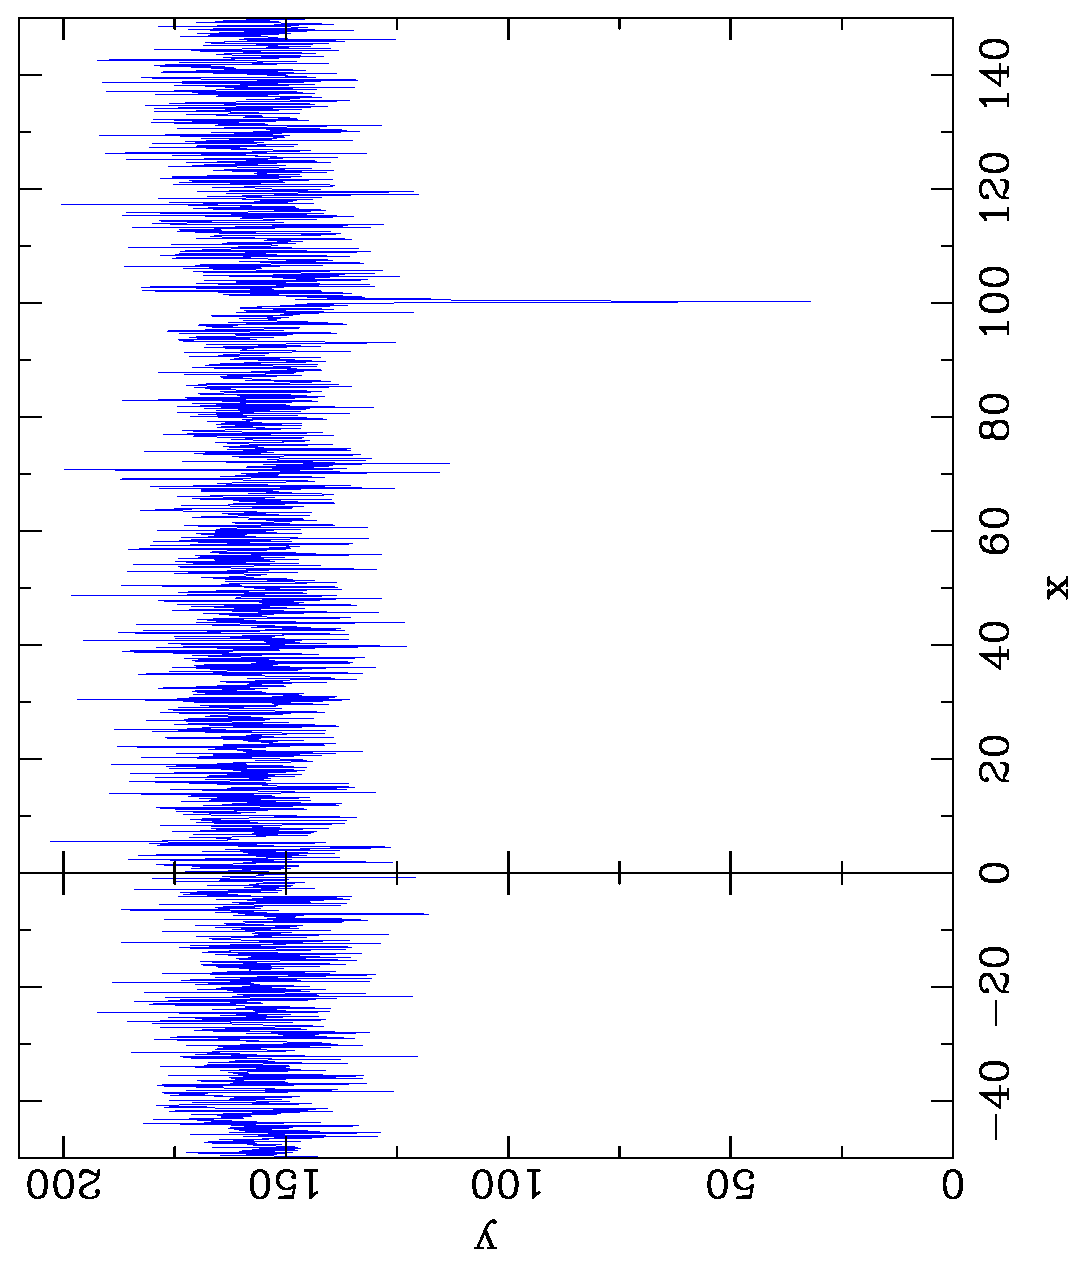
\includegraphics[angle=270,scale=0.45]{example.raw.eps}
   \caption{Example data}
   \label{fexa-arc}
\end{figure}

The function in Fig. \ref{fexa-arc} shall be the data set for the
refinement in this section. The function from which these data were
calculated is:
\begin{equation}
   y ~=~ P_{1} atan \left ( \frac{|x-P_{2}|}{P_{3}}\right)
   \label{eq-exa-arc}
\end{equation}
where atan is the arc tangens or inverse tangens function, and $P_{i}$
are free parameters that determine the behavior of the function. The
function has a minimum y=0 at $x ~=~ P_{2}$. The width of this minimum
depends on $P_{3}$. For small values of $P_{3}$ the minimum is smaller.
Far away from the minimum, the function is almost constant at 
$y ~=~ \pi/2 P_{1}$. The data were generated by adding a Gaussian 
distributed noise to each data point.

\begin{figure}
   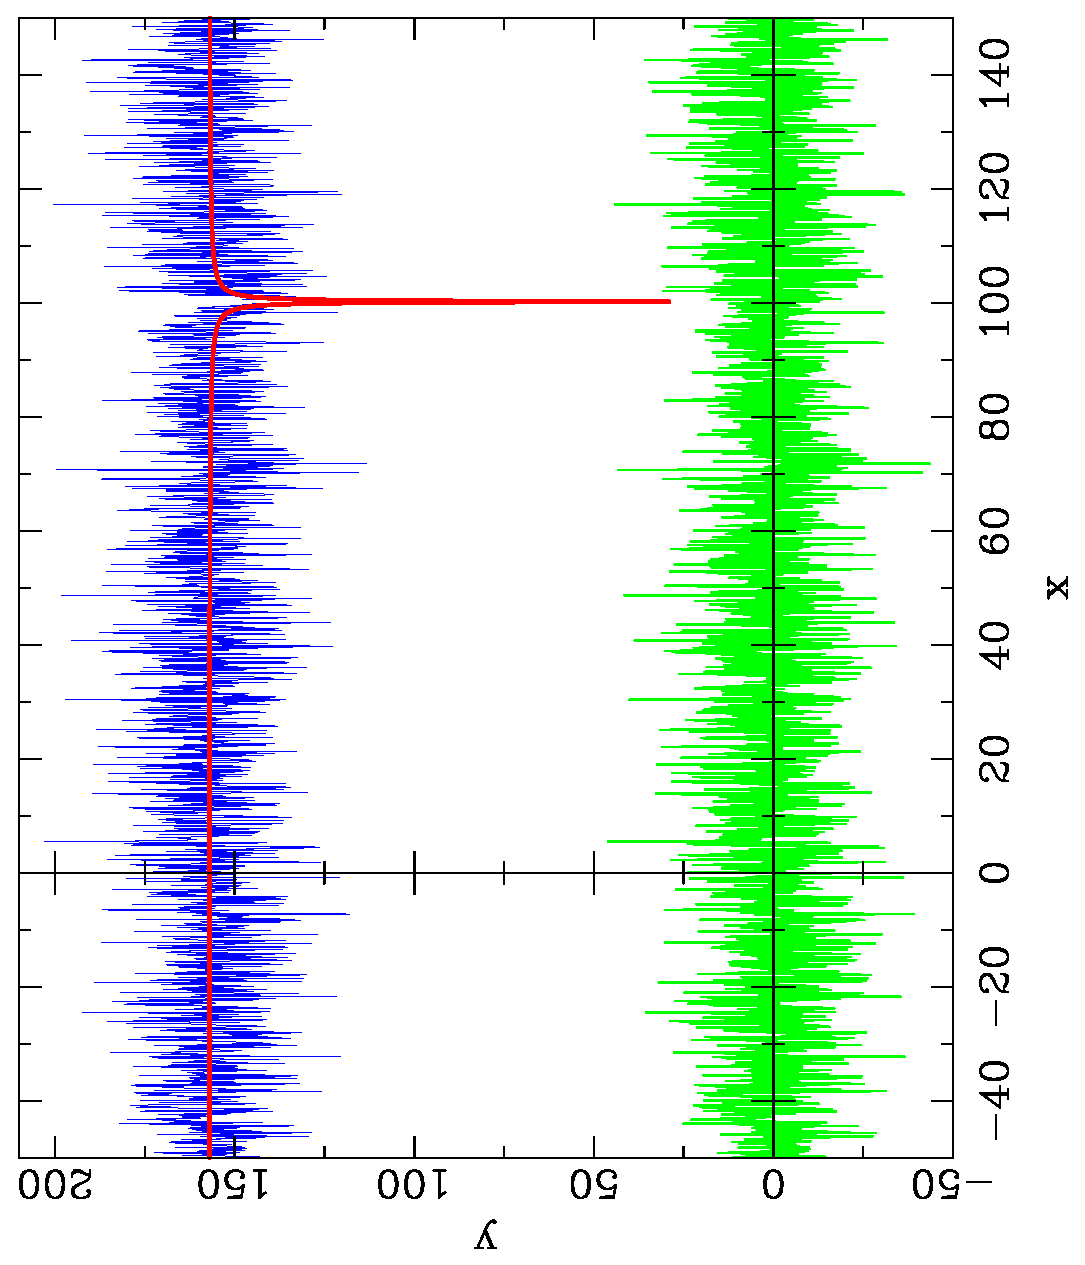
\includegraphics[angle=270,scale=0.45]{example.ideal.eps}
   \caption{Example data in comparison to the ideal function. The
    R-value between the observed and calculated function is 8.18\%.}
   \label{fexa-ideal}
\end{figure}

This data set proves to be a very hard challenge for any least squares
algorithm. Unless the starting values are very close to the actual
values, the least squares algorithm will not find the global minimum.
The very high noise level effectively prevents the algorithm from
finding the position of the minimum. Instead the R-value is minimized
by setting $P_{3}$ to the smallest positive value. At this level, the
width of the function is reduced to one point, if any. Furthermore, the
slope of the function is essentially zero for all x, and the position of
the minimum does not influence the R-value. The R-value is, however,
significantly above the R-value that is achieved for the ideal 
parameter values, show in Fig. \ref{fexa-ideal}.

To refine the function with \diffev, we need to define a couple of
items. These include:
\begin{itemize}
  \item Population size
  \item Limits, starting range etc. for the parameters $P_{i}$
  \item Values for refinement control variables
  \item location and names for files
\end{itemize}

The optimum size of a population is not always straightforward to
estimate. Since the minimum at $P_{1}$ is very narrow, a fairly 
large population size is advisable. A test shows that the population
should consist of approximately 40 members to ensure that the 
minimum is found.  The corresponding commands would be:
\begin{MacVerbatim}
  pop_n[1]   = 40
  pop_c[1]   = 40
  pop_gen[1] =  0
\end{MacVerbatim}
Here the number of members and children was set to the same value,
there is no fixed need to do so, unless the selection mode is set 
to compare a child with its immediate parent. With the last statement
the current generation number is set to zero. If a refinement is to 
be continued, the generation number can be set to the corresponding 
value.

The next group of definitions includes the number of parameters,
and then for each parameter a suitable name, hard boundaries, a
starting range and definitions how to handle parameter behavior 
at the hard boundary and in a local search.

In the current example, we have three parameters, all of which are 
floating numbers. None of the parameters has any absolute lower or
upper boundary imposed by external rules. Parameter $P_{3}$ must
not be equal to zero, this we will handle later as a constraint.
Sensible hard limits for the parameters could be:\\
\begin{tabular}{lp{2cm}p{2cm}p{8cm}}
     parameter & \raggedright{lower boundary}
               & \raggedright{upper boundary}
               & comment\\
     \hline
     1 &   0 & 200 & \raggedright{All data points are larger than zero.}
                     \tabularnewline
     2 & -50 & 150 & \raggedright{Minimum must be somewhere within the 
                                  observed x-range}
                     \tabularnewline
     3 &  -1 &  1  & \raggedright{Include zero to use constraints}
\end{tabular}
\\
\par 
If one has good estimates for the parameter values, these can be used 
to limit the initial spread of the population. A narrow spread of the
initial population around the expected final value will speed up the
convergence. Should these estimates prove to be wrong, however, the 
refinement will take extra long or may fail altogether. Here we will
not impose any prior knowledge on any of the parameters and use the
full range set by the hard boundaries.

During the initial refinement stages, the differences between the 
members will be large and chances are that the donor falls outside 
the allowed hard boundary interval. \Diffev corrects this situation by 
setting the violating parameter to a Gaussian distributed value 
with mean at the hard boundary. The respective half of the Gaussian
distribution that falls inside the boundary range is taken as valid
region. The user can set the sigma for this distribution and define
whether this sigma shall remain constant or be adapted during the
refinement. For parameters 1 and 2 we will set the initial sigma to
1, and for parameter 3 to 0.02. In later refinement cycles the
value of sigma can be adapted to a fraction of the total parameter 
spread, in our example to 0.2 of the parameter spread. 

Similarly, the sigma for a local search is fixed to starting values 
and adapted to a fraction of 0.01 of the total parameter spread.

For parameter 1 this would be set by the commands:
\begin{MacVerbatim}
   pop_name    1,height
   type real,1
   pop_xmin[1] =   0.0
   pop_xmax[1] = 200.0
   pop_smin[1] =   0.0
   pop_smax[1] = 200.0
   pop_sig [1] =   1.0
   pop_lsig[1] =   0.1
   adapt sigma , 1,0.2
   adapt lsigma, 1,0.01
\end{MacVerbatim}

As of version 5.16, \Diffev offers a shortened version of these 
commands with standardized values for the sigmas:
\begin{MacVerbatim}
   newparam height, 0.0, 200.0, 0.0, 200.0
\end{MacVerbatim}

If needed optional parameters can specify more details:
\begin{MacVerbatim}
   newparam height, 0.0, 200.0, 0.0, 200.0, init:keep
   newparam height, 0.0, 200.0, 0.0, 200.0, init:initialize
   newparam height, 0.0, 200.0, 0.0, 200.0, type:integer
   newparam height, 0.0, 200.0, 0.0, 200.0, type:real
\end{MacVerbatim}

This command assumes the {\it good} values sigma = 0.001 and 
local sigma = 0.0001 and will adapt the sigma to a population 
width of 0.2 and the local sigma to 0.02 of the population width.

The command assumes that the parameter is real valued unless the
optional parameter "type" is set to "integer".

Since parameter $P_{3}$ forms the denominator of Eq. \ref{eq-exa-arc},
its value must not be equal to zero. Check the function with a couple 
of different parameters, or simple mathematical analysis 
would show that the product $P_{3}~P_{1}$ must also be larger 
than zero to produce the observed dip. A clear lower limit for 
$P_{3}$ can, however, not be given. Therefore, $P_{3}$ was allowed 
in the interval [-1:1], and we just have to exclude a value of zero.

If the problem is difficult to solve, or if one wants to get a quick
estimate of one parameter, one can choose to refine just a subset. 
Since we only have three parameters, we will refine all at the same
time.

\begin{MacVerbatim}
   constrain p[3].ne.0.0
   refine     all
\end{MacVerbatim}

The next group of definitions concerns the control variables. \Diffev
offers the two basic variables, the scale factor, by which the difference
vector is multiplied, {\tt diff\_f[1]}, and the cross over probability
{\tt diff\_cr[1]}. Both are limited to the interval [0:1]. For this
refinement problem, the actual value of the cross over probability does
not matter, the scale factor should be closer to one to ensure 
successful refinement.

A variation of the basic algorithm allows to add the difference vector to 
any point along the line between parent and donor base.
In this problem, the location does not influence the refinement, and 
we choose the value of 1, which corresponds to the original 
algorithm. Also, the value of the local search probability does not
affect the search efficiency in this example, as long as its value is 
smaller than a value of roughly 0.3, and here it is set to zero.

\begin{MacVerbatim}
   diff_cr[1]  = 0.8
   diff_f[1]   = 0.81
   diff_k[1]   = 1.0
   diff_lo[1]  = 0.0
\end{MacVerbatim}

The next choice concerns selection of the donor. One can either choose 
the current best member as donor, or choose the donor at random. 
Here the donor is chosen at random. 

If the dependency of the R-value on the parameters is a reasonably 
smooth distribution without too many false minima, one can accelerate 
the convergence by taking the combined group of parents and children 
and to choose the best members to form the next set of parents. 
Here this is a good choice.

\begin{MacVerbatim}
   donor      random
   selection  best,all
\end{MacVerbatim}

Finally we need to define filenames for the trial files, the results
and the two log files. To keep the output nicely sorted, these files
are written into a subdirectory {\tt DIFFEV}.

\begin{MacVerbatim}
   trialfile  DIFFEV/Trials
   restrial   DIFFEV/Result
   logfile    DIFFEV/Parameter
   summary    DIFFEV/Summary
\end{MacVerbatim}

This concludes the basic setup. Prior to the main refinement loop, we
just have to generate the initial parameter sets, which is done by
the command {\tt initialize}, which does not take any parameters.
This command sets the current generation number to zero and writes
a first version of all trial files.

\begin{MacVerbatim}
   init
\end{MacVerbatim}

The main refinement follows, usually in a loop over several generations.
Within the loop, the {\tt system} command must be used to execute the 
slave program or programs that calculate the R-value. Once these are 
done, the {\tt compare} command reads all R-values, and generates the
next generation of trial values. It also updates the log files. For a 
fixed number of refinement cycles this could be a construction like:

\begin{MacVerbatim}
   do i[0]=1,40
     system ./arctan
     compare
   enddo
\end{MacVerbatim}

A loop with 40 cycles is executed, using the external program "./arctan"
to calculate the R-values. In a UNIX environment the leading "./" 
specifies that the program {\tt arctan} is found in the current 
directory. Without this specifier, the UNIX shell would search for 
the program in the directories specified by the value of your 
{\em PATH} variable. 

An indefinite loop that requires manual intervention could be:

\begin{MacVerbatim}
   variable integer, terminate
   terminate = -1
   fopen 1, CONTINUATION
   fput  1, terminate
   fclose 1
   do while(terminate.eq.-1)
      system ./arctan
     compare
     fopen 1, CONTINUATION
     fget  1, terminate
     fclose 1
  enddo
\end{MacVerbatim}

The macro initially sets the variable {\tt terminate} to "-1" and 
writes this to the file {\tt CONTINUATION}. The loop is executed
until the value of the variable is no longer "-1". At each cycle
the content of file {\tt CONTINUATION} is read into variable 
{\tt terminate}. Thus, the macro will stop, if you edit this file
and change the number stored within.

Finally, the following macro checks the R-value and reacts accordingly.
The commands in this macro were used to generate the performance 
tests in chapter \ref{diff}.

\begin{MacVerbatim}
  variable integer,cycle
  cycle = 0
  do
    system ./arctan
    compare
    cycle = cycle + 1
  enddo until (bestr[1].lt.0.0817830 .or. cycle.gt.100)
\end{MacVerbatim}

The loop is run indefinitely, until either the R-value has fallen
below a threshold, or until the number of cycles exceeds 100.

\begin{figure}
   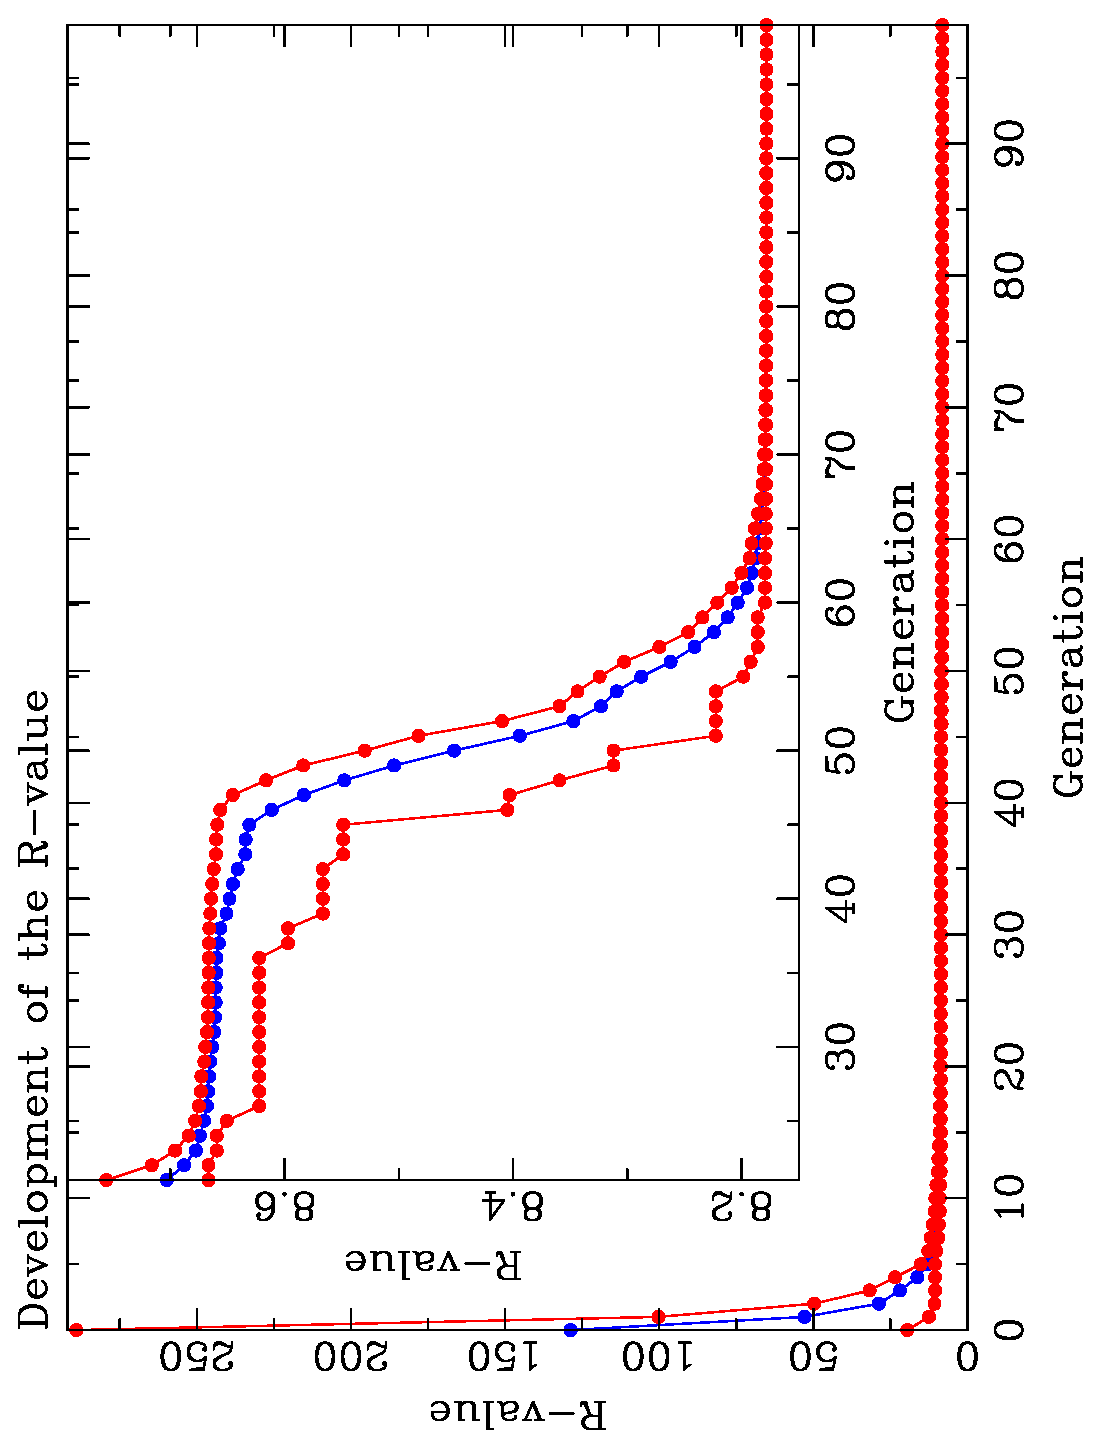
\includegraphics[angle=270,scale=0.45]{example.rval.eps}
   \caption{R-value as function of refinement generation. The Figure
            shows the best, worst R-value (red curves) and the average
            R-value (blue)}
   \label{fexa-rval}
\end{figure}

A typical refinement run is shown in Fig. \ref{fexa-rval}. The
refinement is set according to the control variables described in 
this section. Initially, the best and worst R-values quickly drop
to values around 9 to 12 \%. In these cycles, those parameter 
values that are really far off are eliminated. Thereafter, the 
real refinement starts. Up to generation 37 little change occurs.
At this stage, the first members have found the global minimum, 
and after generation 45 all members begin to converge into the 
global minimum, which is reached after generation 70. Thereafter,
no significant progress occurs.

\begin{figure}
   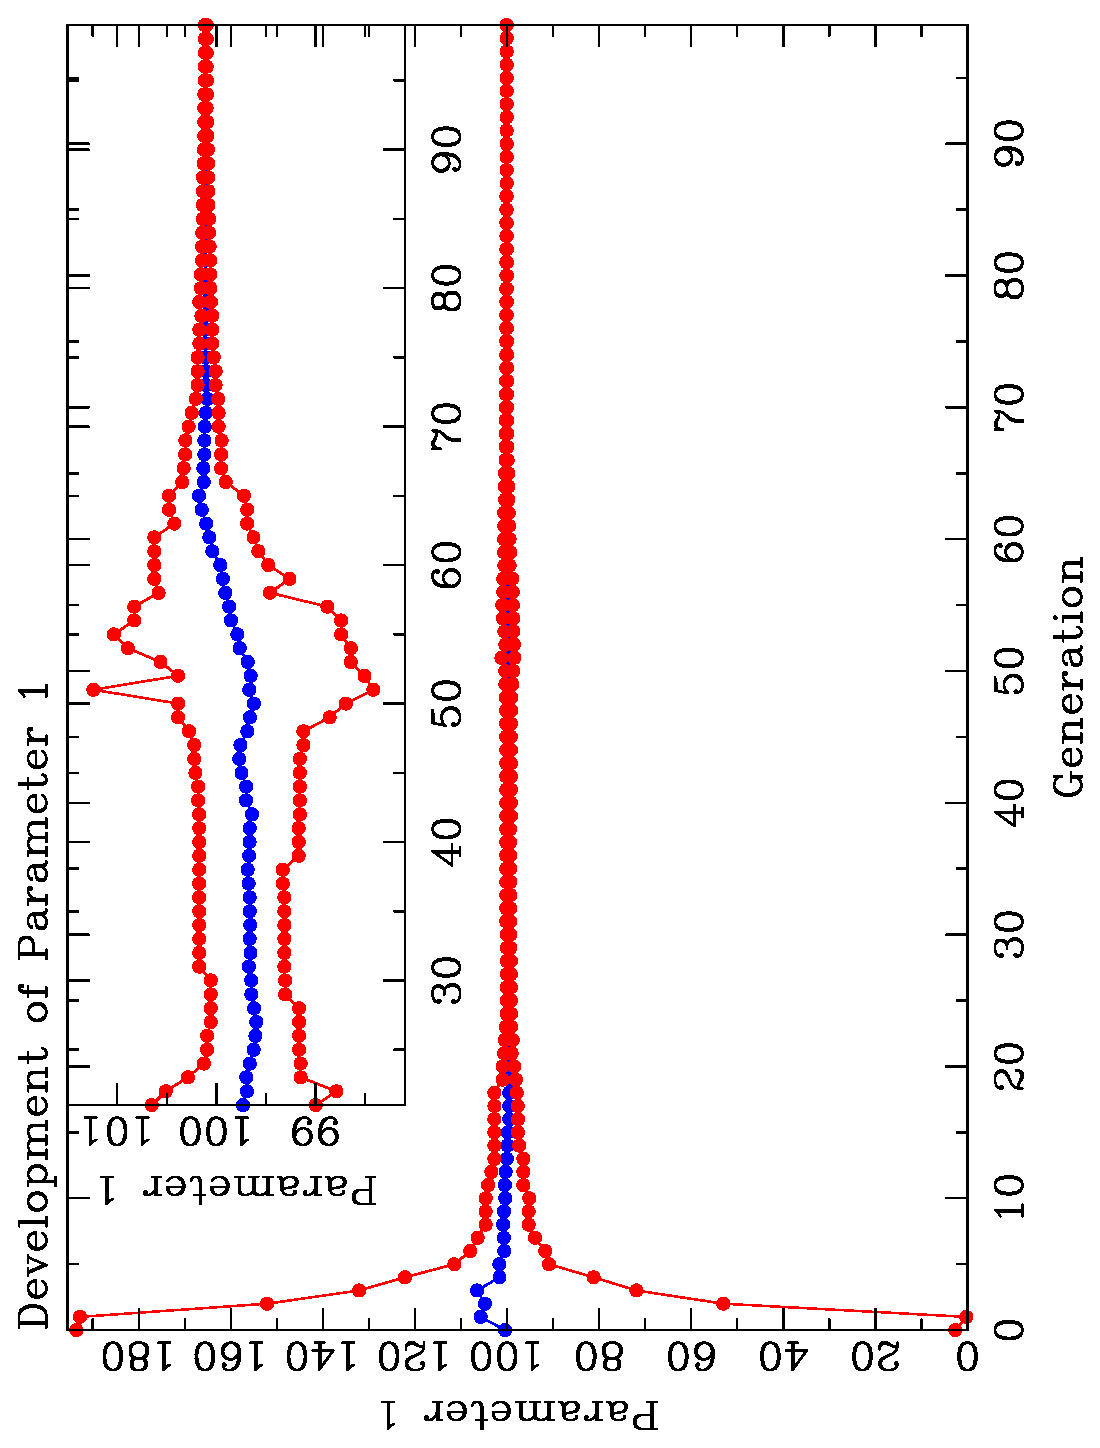
\includegraphics[angle=270,scale=0.45]{example.p1.eps}
   \caption{Parameter P1 as function of refinement generation. The Figure
            shows the best, worst R-value (red curves) and the average
            R-value (blue)}
   \label{fexa-p1}
\end{figure}

The main effect on the R-value is caused by the value of the parameter 
$P_{1}$, Fig. \ref{fexa-p1}, since this parameter lowers or raises 
the function over the 
whole x range. Accordingly, the refinement quickly finds a value close
to the right value. Notice that around generation 50, the parameter values
spread before the final value is found. It is around these generations
that all members find the global minimum and during the adjustment of
parameter $P_{3}$, the other parameters spread out for a few generations.

\begin{figure}
   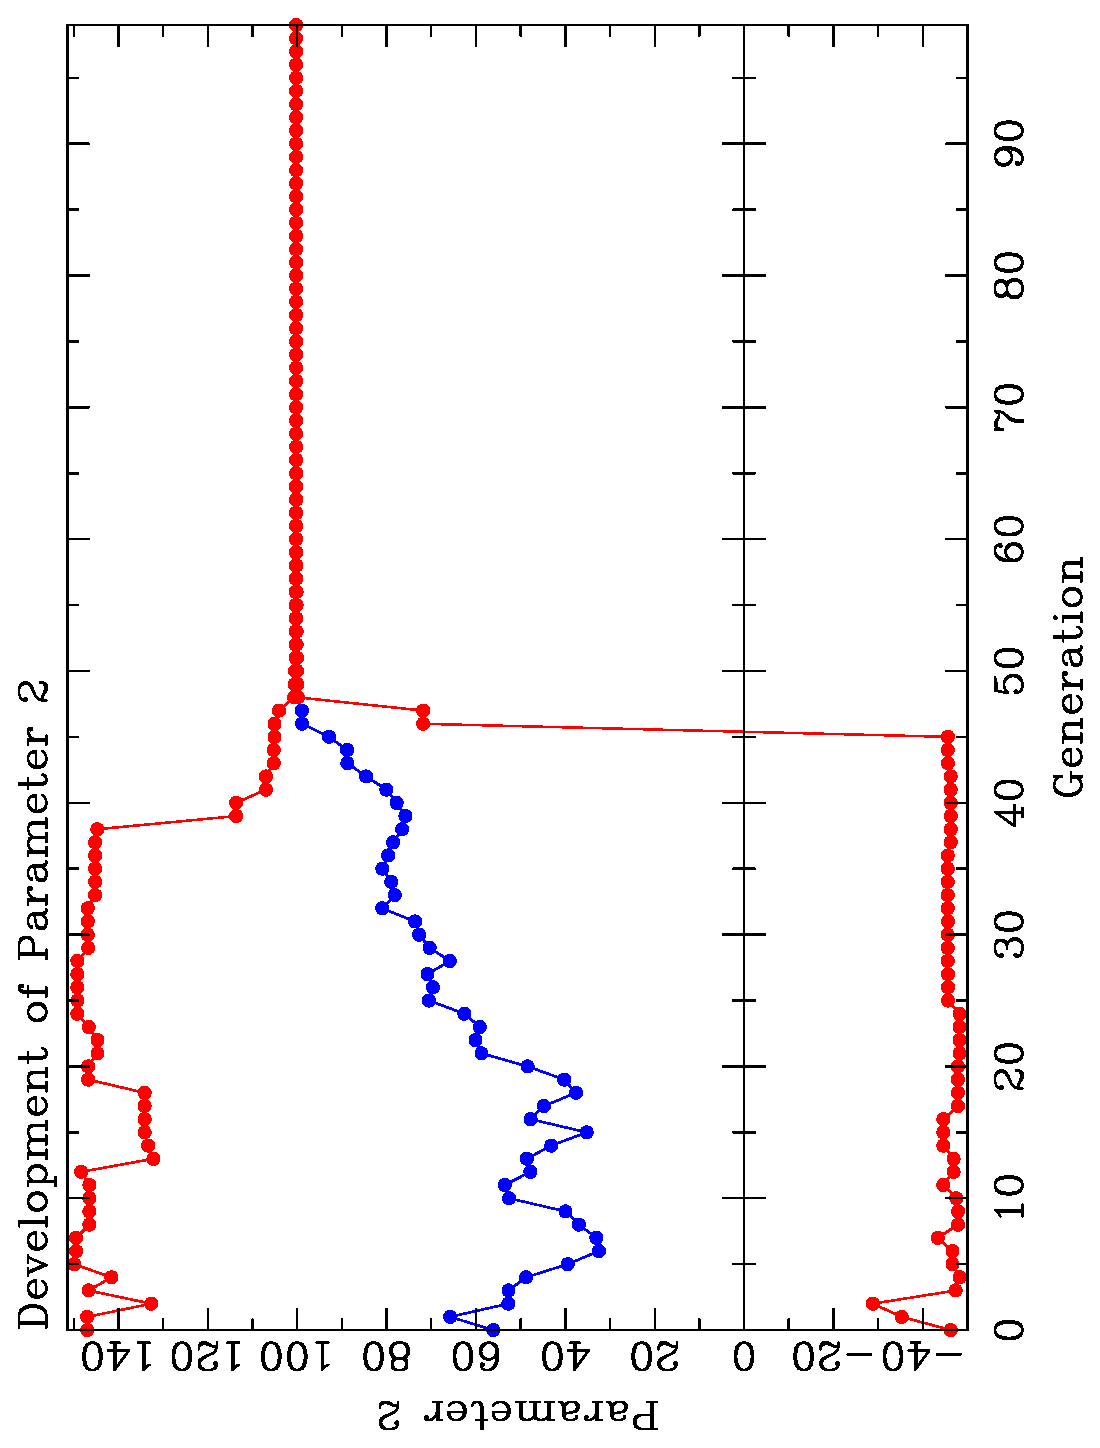
\includegraphics[angle=270,scale=0.45]{example.p2.eps}
   \caption{Parameter P2 as function of refinement generation. The Figure
            shows the best, worst R-value (red curves) and the average
            R-value (blue)}
   \label{fexa-p2}
\end{figure}

For the first roughly 15 generations, the value of parameter $P_{2}$,
Fg. \ref{fexa-p2}, hardly affects the R-value. As long as the position 
of the minimum is
not very close to the true value, its position hardly matters. 
From Generation 20 to 45 more and more members find the correct 
position.

\begin{figure}
   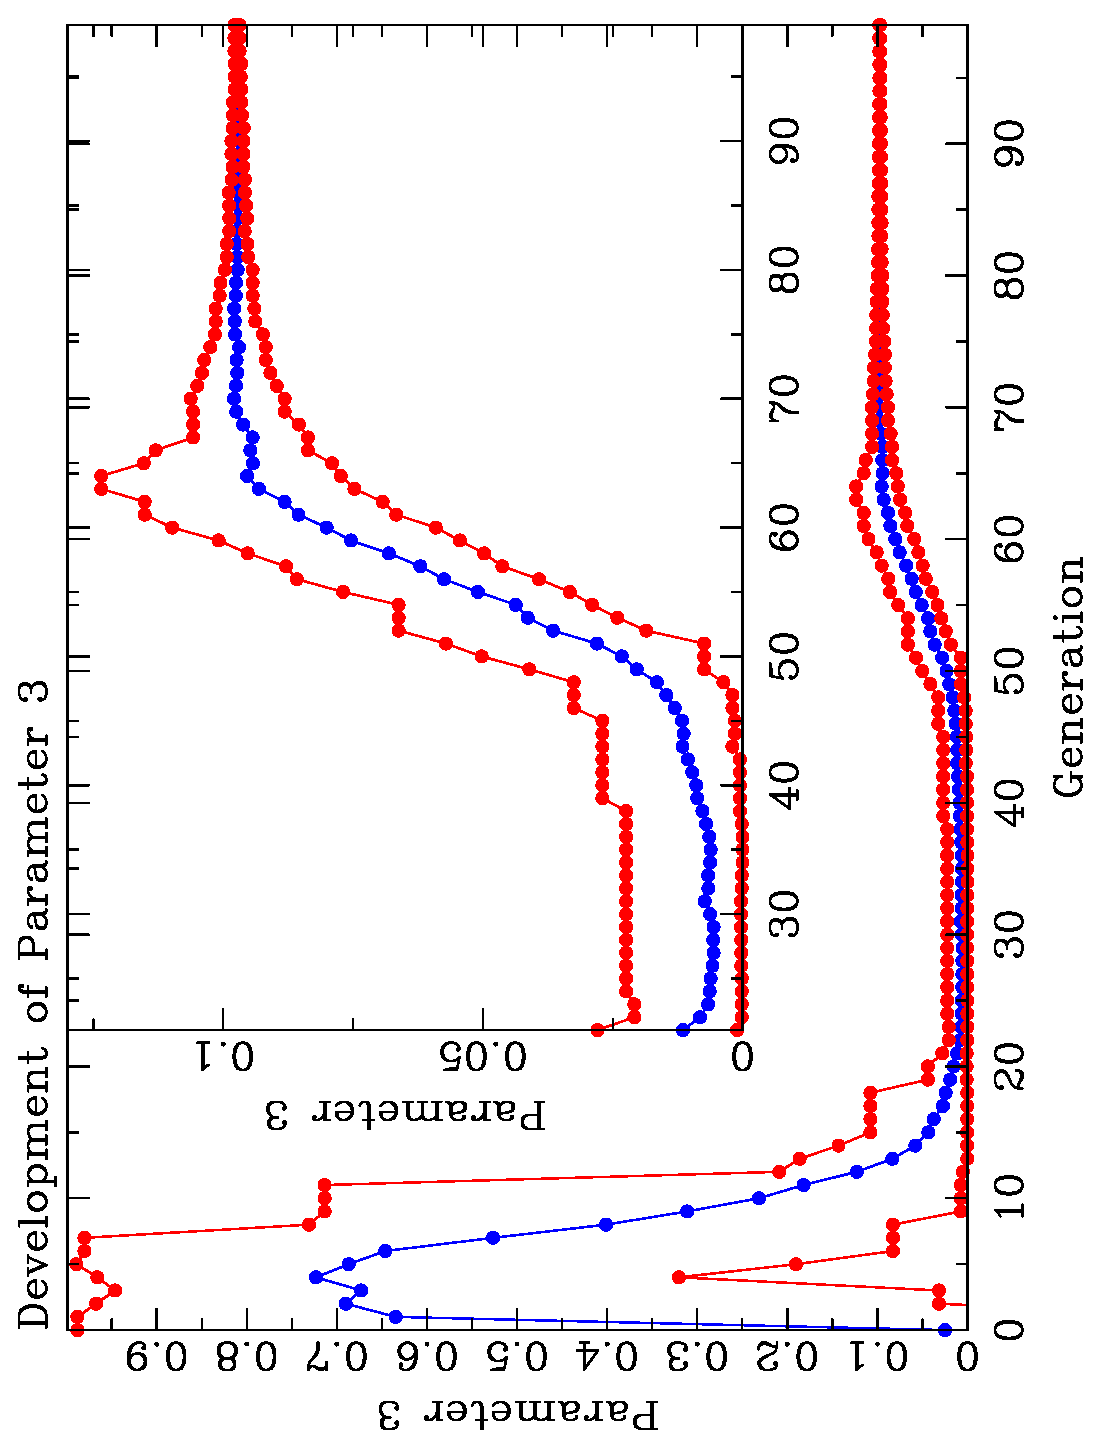
\includegraphics[angle=270,scale=0.45]{example.p3.eps}
   \caption{Parameter P3 as function of refinement generation. The Figure
            shows the best, worst R-value (red curves) and the average
            R-value (blue)}
   \label{fexa-p3}
\end{figure}

Parameter $P_{3}$, Fig. \ref{fexa-p3}, shows the most unusual refinement 
behavior. In the 
first few generation, all members with negative values of $P_{3}$ are
eliminated. The parameter then refines to values between zero and 0.02,
much lower than the true value. As long as the position of the minimum
is not found, lower R-values result if parameter $P_{3}$ is as close
to zero as possible. To get out of this local minimum, a large 
population size is required. Once the correct position is found,
parameter $P_{3}$ also refines to its correct value.

At this stage, the refinement is finished and the calculated curve 
is that of Fig. \ref{fexa-arc}. Admittedly, the difference between
the R-values around generations 30 at 8.65\% are not very 
significantly worse that the final R-value of 8.18\%. This is due to
the large amount of noise in the {\em experimental} data. 
These conditions were, however, chosen on purpose to illustrate
the ability of the differential evolutionary algorithm to jump out
of local minima, even under adverse conditions.

%------------------------------------------------------------------------



%------------------------------------------------------------------------
% Appendices
%------------------------------------------------------------------------

\appendix
\chapter{DIFFEV commands}
\section{News}
\subsection*{2018\_Nov}
\par
Added a new command 'restart $ <$user\_generation$> $' This command compares 
the user value to the current value in GENERATION. If the user 
value is smaller, the Logfiles, Summary and Last files are 
shortened and the GENERATION file is adapted. This lets you step 
back to an earlier refinement status. Keep in mind that the later 
cycles are irrevocably lost. If in doubt make a backup first. 
\par
reinstated the ==$> $ 'read' command 
\par
Added further options to the ==$> $ 'release' command 
\subsection*{2018\_Oct}
\par
Added a ==$> $ 'release' command that is intended to act 
complementary to a previopus ==$> $ 'fix' command. 
\subsection*{2018\_July}
\par
A small modification to the "diffev\_best" macro. 
The value of REF\_NINDIV is written and at the end a 
"set error, continue' instruction has been added. 
\subsection*{2018\_June}
\par
Revised the reaction to a CTRL-C 
\par
Added a ==$> $ 'set error, ... , "save" option 
\par
Revised the internal workings of the distribution within 
run\_mpi. This has no effects on the user. It should anable you, 
however, to distribute the children much better on a system with 
many nodes and many CPU's per node. See the manual for furtrher info. 
\subsection*{2018\_Feb}
\par
Added an optional parameter "partial:$ <$value$> $" to the 
==$> $ 'restrial' command. This parameter tells DIFFEV how many 
partial R-values the slave program will calculate and return. 
If set or if the value is larger than 1, DIFFEV will create 
logfiles "Summary.Rvalue.0001", "Parameter.Rvalue.0001" and 
"Current.Rvalue.0001" etc. for each partial R-value. 
Use the KUPLOT commands 'rval' and 'cost' to set the 
individual R-values and a (weighted) average. 
You can display the development of the partial R-values within 
KUPLOT" with the kuplot command 'kpara'. 
\par
removed 'read' command 
\subsection*{2018\_Jan}
\par
The logical comparisons may now take the operators: 
$ <$, $ <$=, ==, /=, $> $=, $> $/ 
The classical fortran77 operators are still valid 
\par
New logical functions "isvar" and "isexp" can be used within an 
"if" construction. See help entry ==$> $'function' in the 
general "Command\_lang" section 
\par
The ==$> $ function par\_number($ <$char\_variable$> $) returns the 
number for the refinement parameter in the character variable 
$ <$char\_variable$> $. 
\par
The ==$> $ function par\_name($ <$number$> $) returns the name of the 
refinement parameter number $ <$i$> $. 
\par
Finished the transformation from parameter numbers to 
parameter names. All Log files now have an extension of the 
parameter name instead the parameter number. 
\par
The new command ==$> $'reset' can be used to reset DIFFEV to the 
conditions at program start. 
\subsection*{2018\_Dec}
\par
Major revision of the refinement parameter handling. 
The new command 'newparam' effectively replaces for most of the 
common refinements the need of the individual commands to set the 
parameter values. Throughout the command language much more 
epmphasis is placed on the parameter names instead of the 
parameter numbers. See ==$> $'refine' and 'init' commands. 
The parameter names are alos placed into the user variable 
environment and handed down to the slave program (discus or kuplot) 
where they will have the appropriate values for the members of 
the population. 
\par
Added a 'read' command that reads GENERATION and the ==$> $ 'logfile' 
This allows for easier changes of the population size, see the 
entry 'Description / Population\_size' 
\subsection*{2017\_Sep}
\par
Throughout the program the internal calculation of random numbers 
was changed to the FORTRAN 90 intrinsic function. 
\subsection*{2017\_July}
DIFFEV has been modified to log the status of the random number generator 
at the beginning of each slave calculation. This status is documented 
internally for the current best member of the population. Once an 'exit' 
command is executed, DIFFEV will write a macro called "diffev\_best.mac" 
that can be used to recreate the current best solution. 
\subsection*{2017\_Jan}
An unfortunate typing error in News/2016\_Oct regaring the new 
refinement variable 
ref\_para[1...]   ( was misspelled as ref\_param[1...] ) 
is corrected in the  on-line help. 
\par
Another typing error caused a an error in the macro parameters 
transferred with a NON MPI command: run\_mpi, making these 
not backward compatible. This has been fixed. 
\subsection*{2016\_Dec}
\par
At a few select points colors are introduced into the output. 
Currently these are just the error messages. 
\par
\subsection*{2016\_Oct}
\par
Global variables have been introduced that use the same syntax as 
user defined variables. This include just "pi" and variables related 
to the refinement. 
DIFFEV sets the value to these variables: 
REF\_GENERATION  Current generation 
REF\_MEMBER      Current population size 
REF\_CHILDREN    Current children size 
REF\_DIMENSION   Number of parameters 
REF\_KID         Current child Updated for DISCUS and KUPLOT only 
REF\_INDIV       Current individuum Updated for DISCUS and KUPLOT only 
REF\_NINDIV      Number of individual repetitions 
ref\_para[1..]   Current trial parameters for current child 
\subsection*{2016\_june}
\par
DIFFEV may now be interruted gracefully with a CTRL-c. 
This will cause DIFFEV to shut down MPI if active. 
\par
The 'run\_mpi' command can now be used as a generic interface to identical 
slave macros, regardless of the MPI status. 
\subsection*{2016\_april}
\par
The initialise command was augmented by a second form to  initialise 
just the logfiles, see ==$> $ 'logfile', 'summary'. 
This might be helpful if you want to reset the refinent cycle 
to a smaller generation number. For very lengthy refinements with 
a few thousand refinement cycles and many parameters, a continuation 
will take appreciable time to read all previous cycles. If the 
actual development accross the cycles is not relevant to you you 
can reduces the file sizes drastically be a sequence like: 
pop\_gen[1] = 1 
initialise logfile 
\par
New command 'lastfile' 
\par
This new command creates a short copy of the ==$> $ 'logfiles'. 
This short form contains the parameters just for the last 
refinement generation. 
\subsection*{2013\_May}
\par
The run\_mpi command has been augmented by a "socket" qualifier, which 
will cause DIFFEV to run the application program controlled via a 
socket. This should speed up the process on a multi-core/multi-cpu 
system. 
\subsection*{2011\_June}
\par
The program is now a fully functional fortran2003 program. 
There are no changes that must be followed by the user, but important 
differences exist in the memory allocation. The internal arrays that hold 
the population are now all allocated automatically, when you define the 
number of parameters to be refined, the size of the population and the 
constraint equations. Most of the time you will not have to bother with 
these computational details. If you whish, you can allocate appropriate 
array sizes, see ==$> $ 'allocate', 'deallocate'. 
\par
With this version, the program allows the user to change the population 
size and the number of parameters to be refined during a refinement cylce. 
\par
If the number of parameters to be refined in increased during a cycle, 
the program will automatically write new child parameter sets and patch 
the logfile and summary file. 
\par
See the entry ==$> $ "Description" ==$> $ "Increase\_Dimension" for an example. 
\par
Related to this new feature, the ==$> $ "initialize" command now allows to 
(re-)initialise an individual parameter. 
\par
\section{Synopsis}
\par
\begin{MacVerbatim}
Description ! A description of the program
News        ! Information on recent changes
allocate    ! Allocate array sizes
adapt       ! Adaption of global/local search width
backup      ! Backup current best solutions
compare     ! Compares the results of the current population
constraint  ! Defines a constraint condition
deallocate  ! Deallocate array sizes
dismiss     ! Dismiss the worst parents; replace by new children
donor       ! Defines which donor to use
fix         ! Fixes a parameter
initialize  ! Initializes the generation zero
lastfile    ! Defines a file name for the parameters for the last generation
logfile     ! Defines the file name for the parameters for each generation
newparam    ! Defines Ra new parameter or new values for a parameter
pop_name    ! Defines names for the individual parameters
refine      ! Defines which parameters are refined/fixed
release     ! Initialize a parameter that had been fixed
restrial    ! Defines the file name for the current R-values
run_mpi     ! Run the cost function program in parallel through MPI
selection   ! Defines how children/parents survive into next generation
summary     ! Defines the file name for a summary of the parameter changes
trialfile   ! Defines the file name for the current parameters
type        ! Sets the numerical type for a parameter (integer or real)
write       ! Writes new Children or new GENERATION file
\end{MacVerbatim}
\section{Description}
\par
The program DIFFEV uses the differential evolution algorithm to refine 
a set of parameters to a set of observations. 
\par
DIFFEV provides the handling of the parameters and their evolution. 
An external program must be used to calculate the cost function or 
R-value that corresponds to a given set of parameters. 
\par
The differential evolution algorithm compares simultaneously the resulting 
cost function for several sets of parameters. The number of parameter sets 
is called the population. For each member of the population a set of 
parameters is used. This is called a parameter vector. Its dimension 
depends on the model that you need to describe. In order to describe 
a parabola you would need three parameters. The whole set of parameters 
is called a generation. 
\par
For each generation, the cost function is evaluated for each member of 
the population. The next generation is determined from the current 
parent generation through the following procedure: 
\par
Loop over all members 
  - Choose a member (at random or at will), this will be the 
    donor base. 
  - Set a point along the line between current member and donor base 
    to create the effective donor base ==$> $ diff\_k[1] 
  - Select two other members by random choice 
  - Loop over all parameters: 
     - Take the difference between the corresponding parameters of the 
       two other randomly chosen members. 
     - Multiply this difference by a user provided value ==$> $ diff\_f[1]. 
     - Add the difference vector to the effective donor base to 
       create a parameter set called the donor. 
       - One parameter of the donor is always chosen for the child. 
         All other parameters are then randomly chosen from: 
         Either:  the parent 
         Or    :  the donor 
       - The probability for this choice is weighted by a user provided 
         probability ==$> $ diff\_cr[1]. 
\par
Once a new generation has been determined the corresponding cost function 
is calculated. 
\par
Next the selection process determines, which current children survive 
into the next generation. This is done either by: 
- Direct comparison between a parent member and its immediate child. 
  Only those new members survive, whose cost function is 
  less than that of the parent. Otherwise the parent is retained. 
- All parents and all children are pooled into one set. From this set 
  the best members survive, irrespective whether they were a parent 
  or a child. 
\par
Such an algorithm is able to search for parameters if a standard refinement 
algorithm fails or is difficult to adapt. This might be the case for: 
- Undefined parameter values within the possible range. The parameter 
  P may for example NOT be equal to 1 for a function: 1/(1-P) but values 
  larger AND smaller are allowed. 
- The calculation of the cost function involves existing extensive 
  algorithms or several different programs. 
- The calculation involves the averaging of several calculations that 
  rely on data created by (Gaussian-) randomly distributed parameters. 
\par
Files 
\par
DIFFEV uses several files to store the parameter values, the current 
status etc these are: 
\par
"GENERATION"   Fixed file name in the current directory! 
\par
The file "GENERATION" contains twelve fixed lines with the current 
generation number, and all relevant file names. 
Further lines contain the backup file names if defined, the random 
number seeds and the finally the parameter names and their allowed 
numerical ranges. 
\par
\begin{MacVerbatim}
 # generation members children parameters
      158        45        90         4
 # trial file
 DIFFEV/Trials
 # result file
 DIFFEV/Results
 # log file
 DIFFEV/Parameter
 # summary file
 DIFFEV/Summary
 # last    file
 DIFFEV/Current
\end{MacVerbatim}
Trial files (obsolete) 
\par
DIFFEV writes a short file for each member that contains the current 
parameters for one member. 
The user defined filename is appended by a four digit member number. 
The first lines contain the information 
on current generation number, the number of members in the population, 
the number of children and the number of parameters 
\begin{MacVerbatim}
# generation members children parameters
     181        45        90         4
# current member
    1
# parameter list
    0.8284027688E-02
    0.5815573883E+02
    0.2050311089E+01
    0.3000000000E+01
\end{MacVerbatim}
Result files (obsolete) 
\par
DIFFEV expects to read the R-values for each member from a short file. 
The user defined filename is appended by a four digit member number. 
\par
The file must contain the member number and the R-value in free format 
within the first line. 
\par
Parameter files 
\par
For the R-value and for each parameter a SPEC type file is written that 
contains all old R-values and parameters, respectively. 
Each generation makes up a scan. The first column is the member number, 
the second column is the R-value and the third column is the respective 
parameter value. 
The base name of the parameter files can be set by the user via command 
==$> $ 'logfile'. As of Version 5.16.1 the base name is appended by an 
extension that is identical to the parameter name. Parameter file 
$ <$name$> $.Rvalue has the same structure, except that both column two and 
three are the R-values. 
\par
Prior to version 5.16.1 the base naem was appended by a four digit 
number with leading zeros. Parameter file no 0000 has the same 
structure, except that both column two and three are the R-values. 
\par
Last file 
\par
A short copy of the parameter file that contains the parameters 
just for the last generation. 
\par
Summary files 
\par
For the R-value and for each parameter a SPEC type summary files 
contains a single scan. Each generation creates one line within the 
scan. Five values arew written to each line. The first column is the 
generation number 
For the R-value and each of the parameters four further columns are 
written. The first of these is the average value, the second the 
minium value, the third the maximum value and the fourth the sigma of 
the parameter distribution. 
The base name of the summary files can be set by the user via command 
==$> $ 'summary'. This base name is appended by a four digit number with 
leading zeros. Summary file no 0000 has the same structure, except that 
both column two and three are the R-values. 
\par
Further help topics are: 
\par
\subsection*{Basic\_Example}
\par
This example illustrates the commands to refine the three parameters 
that describe a parabola: y = P1*x**2 + P2*x + P3 
\par
You will find the data and the macros in the diffev/Example directory 
within the program source directories. 
\begin{MacVerbatim}
======================diffev.mac======================================
#
#
pop_gen[1]  = 0         # initialize the current generation to zero
#
pop_n[1]    = 15        # The population shall have 15 members
pop_c[1]    = 15        # The population shall have 15 children
pop_dimx[1] = 3         # We need three parameters
#
pop_name      1,square  # The parameter is called "square"
#
type          1,real    # Parameter 1 is a floating number
#
pop_xmin[1] = -1.0      # The first parameter is restricted to the
pop_xmax[1] =  1.0      # range -1 to +1
#
pop_smin[1] = -0.8      # The starting parameters of the first parameter
pop_smax[1] = +0.8      # are restricted to the range -0.8 to +0.8
#
pop_sig[1]  =  0.02     # The sigma of minimum parameter "noise".
pop_lsig[1] =  0.002    # The sigma for local searches
#
adapt  sigma, 1, 0.025  # After generation 0 the value of pop_sig[1]
#                       # is adjusted to 0.025*(largest parameter -
#                       #                       smallest parameter )
#
adapt lsigma, 1, 0.0025 # After generation 0 the value of pop_lsig[1]
#                       # is adjusted to 0.0025*(largest parameter -
#                       #                        smallest parameter )
#
pop_name      2,linear
pop_xmin[2] = -2.0
pop_xmax[2] =  2.0
pop_smin[2] = -1.8
pop_smax[2] = +1.8
#
pop_name      3,constant
pop_xmin[3] = -5.0
pop_xmax[3] =  5.0
pop_smin[3] = -4.8
pop_smax[3] = +4.8
#
constraint  p[1].lt.1.3 # Several constraint may be imposed on the
constraint  p[2]+p[3].gt.0.0
#                       # parameters. Here the first parameter must be
#                       # less than 1.3. In the second constraint condition,
#                       # The sum of the second and third parameter must be
#                       # greater than zero.
#
diff_cr[1]  = 0.9       # The cross over probability is 90%
diff_f[1]   = 0.81      # The difference vectors are multiplied by 0.81
diff_k[1]   = 1.0       # For diff_k = 1, the difference vector is added
#                       # to the donor, for diff_k = 0 to the parent.
diff_lo[1]  = 0.1       # In 10% of all cases, a member creates its child
#                       # not by diffev algorithm, but from a local Gaussian
#                       # distributed search.
#
trialfile  silent       # Instead of writing to a file DIFFEV will pass the
#                       # values silently down to DISCUS/KUPLOT
restrial   silent       # Instead of reading a resultfiel, DIFFEV wil
#                       # obtain the cost function results directly from
#                       # the slave program.
logfile    Parameter    # The log file for the parameters
summary    Summary      # A shorter log file
#
init       silent       # Initializes diffev, Generation zero is written.
#
do i[1]=1,15            # A loop over 15 generations
  run_mpi kuplot, kcompare.mac, 0,  /dev/null
#                       # diffev starts the kuplot program with input
#                       # from file "kcompare.mac". This macro instructs
#                       # kuplot to read the 'trialfiles', to calculate the
#                       # cost function for each member and to write the
#                       # results into the 'restrial' files.
#
  compare  silent       # diffev reads the 'restrial' files, compares the
#                       # cost functions of children and parents and
#                       # creates the next generation.
#
enddo                   # End of the loop
\end{MacVerbatim}
\subsection*{Increase\_Dimension}
\par
Here is an example for a macro that should be used to increase the 
number of parameters to be refined: 
\par
\begin{MacVerbatim}
newparam cube, -5.0, 5.0, -4.8, 4.8, keep:initialize
#                                # Defines a new parameter called "cube"
#                                # that is allowed to be in
#                                # the range [-5:+5]
#                                # It is initialized in the
#                                # range [-4.8:+4.8]
dismiss          pop_n[1]/2      # Set R-value of half the population
                                 # to a very high value, thus they will
                                 # be replaced in the next generation
\end{MacVerbatim}
Prior to version 5.19 the macro would have taken the following command: 
\par
\begin{MacVerbatim}
variable integer, ipar           # just a nice variable name
pop_dimx[1]    = pop_dimx[1] + 1 # increase dimension
ipar           = pop_dimx[1]     # copy into variable

pop_name         ipar,cube       # Define name etc for new parameter
pop_xmin[ipar] = -5.0
pop_xmax[ipar] =  5.0
pop_smin[ipar] = -4.8
pop_smax[ipar] = +4.8
type real,       ipar
refine           ipar            # Set refinement flag
init             ipar            # Initialize just this new parameter
dismiss          pop_n[1]/2      # Set R-value of half the population
                                 # to a very high value, thus they will
                                 # be replaced in the next generation
\end{MacVerbatim}
\subsection*{Hints}
\par
These are some hints regarding useful parameters. They are derived 
from the authors experience and are to be carefully adopted. 
\par
The population size MUST be at least 4! 
\par
The population size should be at least about ten times as large as the 
number of parameters, twenty times will give you a good sampling of the 
parameter space. A smaller population runs the risk of converging into 
a local minimum. 
\par
The cross over probability ==$> $diff\_cr[1] should be about 0.8 
 A smaller value (lets say around 0.3), seems to prevent convergence, 
   While a small value prevents the special properties of the 
   differential algorithm to be applied at all. At diff\_cr[1]=0, 
   all children would always be identical to their parents! 
\par
The multiplier for the difference vector ==$> $ diff\_f[1] should be 
around 0.8 
   A small value prevents the children from being very different 
   from their parents, while a large value ~$> $ 1.5(?) seems to 
   prevent convergence, since all children always jump too far away 
   from their parents. 
\par
selection mode 
   If the dependency of the cost function/R-value on the parameters 
   is (or seems to be) fairly straightforward, the convergence is 
   much faster if you choose the selection best,all scheme. By increasing 
   the number of children in comparison to the parents, the selection 
   pressure also increases and the algorithm will move faster into 
   the minimum. This will, however, also happen if you happen to be close 
   to a local minimum, instead of the global minimum! 
\par
I cannot give a hint regarding the number of generations required. 
This depends too much on the problem at hand, parameter correlation, 
the initial choice of parameters etc. 
\subsection*{Population\_size}
\par
Usually the population size will remain fixed during the course of 
a refinement. The population size is defined by setting appropriate 
values to the variable 'pop\_n' and 'pop\_c' for the parent and 
children respectively. 
\par
If you want to change the population size during a refinement, use 
a sequence of commands as follows: 
\par
read         ! This forces DIFFEV to update the parameters from 
             ! GENERATION and the logfiles 
pop\_n[1] = $ <$new\_value$> $ 
pop\_c[1] = $ <$new\_value$> $ 
\par
You may increase or decrease the population size as needed. 
\section{allocate}
{\bf allocate \par }
{\bf allocate "default" \par }
{\bf allocate "constraint", $ <$max\_constr$> $ \par }
{\bf allocate "population", $ <$max\_members$> $, $ <$max\_parameters$> $ \par }
{\bf allocate "show" \par }
\par
\vspace{3pt}
DIFFEV allows to to allocate memory for the arrays needed to store the 
population and the constraints. DIFFEV will dynamically allocate 
the population size, the number of refinement parameters and the 
number of constraints. 
Thus one often may not have to use this command. 
\par
If previously allocated arrays are reallocated, DIFFEV tries to save 
the old values and you can continue to use these. If the new array 
sizes are smaller than the previous ones, this can obviously not be 
done. DIFFEV will perform the new allocation, but all old data are lost. 
A short warning will be printed. 
\par
{\bf allocate \par }
{\bf allocate "show" \par }
\par
\vspace{3pt}
Without parameter or with the parameter "show", the allocate command 
shows the current memory allocations. 
\par
{\bf allocate "default" \par }
\vspace{3pt}
Allocates all array sizes to default values. 
\par
{\bf allocate "constraint", $ <$max\_constr$> $ \par }
\par
\vspace{3pt}
Allocates the maximum number of constraints that DIFFEV shall handle. 
\par
{\bf allocate "population", $ <$max\_members$> $, $ <$max\_parameters$> $ \par }
\vspace{3pt}
Allocate the maximum population size and the maximum number of 
parameters that can be refined. 
\section{adapt}
{\bf adapt "sigma" ,$ <$parameter\_number$> $,[,$ \{$"yes"$| $"no"$| $$ <$value$> $$\} $] \par }
{\bf adapt "lsigma",$ <$parameter\_number$> $,[,$ \{$"yes"$| $"no"$| $$ <$value$> $$\} $] \par }
\par
\vspace{3pt}
DIFFEV uses to "sigmas" to handle special situations. 
\par
The global sigma pop\_sig[$ <$i$> $] is used in the following two situations: 
- a new parameter falls outside the range allowed by pop\_xmin[$ <$i$> $] and 
  pop\_xmax[$ <$i$> $]. In this case the new parameter is chosen by adding a 
  Gaussian random distributed value with sigma pop\_sig[$ <$i$> $] next to the 
  respective boundary. 
- the difference between two parameters is zero. This will usually 
  occur for integer parameters only. In this case the new parameter is 
  chosen by adding a Gaussian random distributed value with sigma 
  pop\_sig[$ <$i$> $] to the value of the effective donor. 
\par
If sigma is allowed to adapt during the fit, its value is set to 
(maximum parameter value - minimum parameter value) * $ <$value$> $ 
Thus, as the population converges to a smaller parameter spread, sigma 
dynamically becomes smaller as well. 
\par
The adaptation can be set for each parameter $ <$parameter\_number$> $ 
separately. 
\par
The local sigma is used to modify a member not by differential evolution, 
but by a adding a local shift to the member. The local shift is a 
Gaussian distributed random value with sigma = $ <$lsigma$> $. 
Whether DIFFEV uses this mode, is determined  by the ==$> $ variable 
diff\_lo[1]. This gives the probability, that a given member will be 
modified by the local change instead of differential evolution. 
\section{backup}
{\bf backup "NONE" \par }
{\bf backup $ <$input$> $ [,$ <$extension] , $ <$output$> $ \par }
\par
\vspace{3pt}
This command allows you to back up the current best solutions. 
Diffev expects that the current trial solutions are called 
inputfile.???? 
or 
inputfile.????.extension 
where "????" is a four digit integer number with leading zeros. 
Note that the '.' before the number "????" and before the extension 
are mandatory parts of the filename. You need to ensure that your 
version of "kup.diffev.mac" adheres to this standard. 
If the output file name includes a path, make sure that the output 
directory does exist. DIFFEV does not create the output directory. 
\par
\par
Examples 
backup CALC/calc, FINAL/final 
This form will back up the files 
      "CALC/calc.????" as "FINAL/final.????" 
backup TEMP/calc, tth, FINAL/final 
This form will back up the files 
      "TEMP/calc.????.tth" as "FINAL/final.????.tth" 
\par
If multiple files need to be backed up, use the 'backup' command 
repeatedly: 
\par
backup TEMP/calc, tth,    FINAL/final 
backup TEMP/calc, grcalc, FINAL/final 
These two lines will back up the files 
      "TEMP/calc.????.tth"    as "FINAL/final.????.tth" 
      "TEMP/calc.????.grcalc" as "FINAL/final.????.grcalc" 
\par
backup NONE 
  Turns off the back up option 
\par
The backup option is useful, if the calculation of the solutions 
takes a long time and involves random configurations. In these cases, 
the extra time required to copy the files may outway the time to 
calculates these again after the end of the refinement. 
If the calculation involves random configurations, a repeated 
calculation of the solutions on which the cost function depends 
may not yield exactly the same result. With the backup option you 
ensure that you always have those backed up solutions correspond 
to the actual cost function values that DIFFEV used. 
\par
If the calculation of the solutions is quick or if it does not 
involve random configurations it is faster not to run the backup 
during the refinements. 
\section{branch}
{\bf branch kuplot [, "-macro" $ <$macro\_name$> $ [ $ <$par1$> $ [ , $ <$par2$> $ ...]]] \par }
{\bf branch discus [, "-macro" $ <$macro\_name$> $ [ $ <$par1$> $ [ , $ <$par2$> $ ...]]] \par }
\par
\vspace{3pt}
Active within the discus suite only! 
\par
Branches to the "kuplot" or "discus" section. 
\par
Within this section any standard KUPLOT command can be 
given. The behaviour of "kuplot" is essentially the same 
as in the stand alone version. Likewise for DISCUS. 
\par
The main use will branch to KUPLOT while the discus section 
is run via run\_mpi from a DIFFEV slave. 
\par
Optionally the "-macro" qualifier instructs the suite to run the 
macro $ <$macro\_name$> $ (with its optional parameters) before the 
interactive session is started. 
\section{compare}
{\bf compare ["silent"] \par }
\par
\vspace{3pt}
This is the main part of the differential evolution section. 
This command reads the current results that the slave program stored 
in files ==$> $ 'restrial' and compares these to the results of the 
parent generation. A new set of children is calculated according to 
the differential evolution algorithm. The successful parents are 
written to the file ==$> $ 'logfile', which stores their respective cost 
function, and the full parameter set. At the same time the short summary 
file ==$> $ 'summary' is appended with abbreviated information about the 
last generation.  The new children parameters are 
written to the temporary files ==$> $ 'trialfile'. The current 
generation is increased in file 'GENERATION'. 
\par
If the optional "silent" qualifier is specified, DIFFEV will not read 
the result files. Instead, DIFFEV must have received the current results 
by explicitly setting the values of child\_val[*] for all children. 
This option will work only within the discus\_suite, which is a 
collection of DIFFEV, DISCUS, and KUPLOT into a common program. 
\section{constraint}
{\bf constraint $ <$logical expression$> $ \par }
\par
\vspace{3pt}
The parameter range may be restricted by defining one or several constraint 
conditions. Each condition must be a valid logical expression. For 
details of the syntax see the manual entry under ==$> $ Command language. 
The parameters within the condition are referred to by p[$ <$i$> $], where 
$ <$i$> $ is parameter number, 1 up to the dimension of the problem at hand. 
The dimension is fixed through parameter ==$> $ 'pop\_dimx', see the 
variable entry. 
\par
Example 
\par
\begin{MacVerbatim}
constraint  p[1].gt.2   # The first parameter must be larger than 2
constraint  4.le. p[2]**2 + p[3]**2
                        # The sum of parameters 2 and 3 squared must be
                        #  equal or greater than 4.
\end{MacVerbatim}
If a constraint equation is not met, DIFFEV will create a new parameter 
set. This process is repeated until a valid parameter set is found, or 
until DIFFEV has tried so for MAX\_CONSTR\_TRIAL times. In this latter 
case the program stops. 
\section{deallocate}
{\bf deallocate $ \{$"all" $| $ "constraint" $| $ "population"$\} $ \par }
\par
\vspace{3pt}
This command allows to deallocate memory for the specified program 
segments. This helps to conserve memory, if program sections are no 
longer needed. 
\par
This deallocation applies to memory that you allocated yourself 
and also to memory that DIFFEV has allocated automatically during 
runtime. As DIFFEV does not necessarily know, when you do not need 
the results of certain calculations any longer, it does not 
deallocate the automatically allocated memory sections unless you 
tell DIFFEV to do so. 
\par
\begin{MacVerbatim}
"constraint"
\end{MacVerbatim}
   Free memory associated to the maximum number of constraints. 
\par
\begin{MacVerbatim}
"population"
\end{MacVerbatim}
   Free memory associated to the population size and maximum number 
   of refineable parameters. 
\section{dismiss}
{\bf dismiss $ \{$$ <$n$> $ $| $ "all" $\} $ \par }
\par
\vspace{3pt}
Set the R-value of the worst $ <$n$> $ parents to a very high value. 
Thus $ <$n$> $ of the next children will definetly have a better R-value 
and replace these parents. 
\par
This command should be used after you changed the parameter dimension 
and initialised ==$> $ 'init' some or all of the trial values. 
Otherwise, many or eval all of the new children might not have 
a better R-value than their parents, and as a consequence the 
(re-)initilization of the trial values may get lost. 
\section{donor}
{\bf donor $ \{$"best" $| $ "random"$\} $ \par }
\par
\vspace{3pt}
The donor vector may be chosen in two different ways. 
"best" chooses the parent member that has the best parameter set. 
"random" chooses at random one of the parent vectors as donor vector. 
Two other parent vectors are always chosen at random to form the 
difference vector that is added to the donor vector. 
DIFFEV chooses the effective donor base along the straight line 
from the current parent vector to the donor. The point along this 
line is determined by the value of "diff\_k[1]" (==$> $ variables). 
For diff\_k[1] = 0  the effective donor is the parent vector, 
for diff\_k[1] = 1  the effective donor is the donor vector itself. 
\section{fix}
{\bf fix $ <$parameter\_no$> $, $ \{$$ <$value$> $ $| $ "best"$\} $ \par }
{\bf fix $ <$parameter\_name$> $, $ \{$$ <$value$> $ $| $ "best"$\} $ \par }
\par
\vspace{3pt}
This command fixes the value of parameter $ <$parameter\_no$> $ or 
$ <$parameter\_name$> $ to 
$ <$value$> $ for all members of the population. The ==$> $ refine 
flag is turned of for this parameter. 
If the second parameter is "best", the parameter is set to the 
corresponding value of the current member with the best R-value. 
\par
As a side effect, the values of pop\_xmin, pop\_xmax, 
pop\_smin, pop\_smax are fixed to this new value as well. 
\section{functions}
\par
The following DISCUS specific functions exist. For a listing 
of general intrinsic functions see help entry 'functions' in 
the 'Command language' section of the online help. 
\par
{\bf par\_number($ <$char\_variable$> $) \par }
\par
\vspace{3pt}
Returns the number of the refinement parameter whose name is 
encoded in the character variable. 
Example: 
line = 'P\_length' 
eval par\_number(line) 
\par
{\bf par\_name($ <$number$> $) \par }
\par
\vspace{3pt}
Returns the name of the refinement variable number $ <$number$> $ 
\section{initialize}
{\bf initialize [ $ <$par\_number1$> $ [, $ <$par\_number2$> $]] [, "silent"] \par }
{\bf initialise "logfile" \par }
\par
\vspace{3pt}
This command initializes the differential evolution sequence. 
\par
Before using this command, you must have defined: 
\begin{MacVerbatim}
Number of parameters to be defined ==> 'pop_dimx'
Size of the parent population      ==> 'pop_n'
Size of the children population    ==> 'pop_c'
Boundaries for each parameter      ==> 'pop_xmin'
                                   ==> 'pop_xmax'
Starting intervals for parameters  ==> 'pop_smin'
                                   ==> 'pop_smax'
Sigmas for parameter adjustment    ==> 'pop_sig'
Local sigmas                       ==> 'pop_lsig'
Cross over probability             ==> 'diff_cr'
Fraction of the difference vector  ==> 'diff_f'
Point between parent an donor base ==> 'diff_k'
Local search probability           ==> 'diff_lo'
\end{MacVerbatim}
Without the optional parameters, 'initialize' is used to start 
the generation zero. 
\par
'Initialize' will use this information to generate the zero's generation. 
The file 'GENERATION' is set to generation zero, the population size 
and the number of parameters is written. 
The files ==$> $ 'logfile' and 'summary' are initialized. Old versions 
with the same name are overwritten! 
The starting parameter values are written to files ==$> $ 'trialfile' 
After the header, each line contains a one parameter, 
'pop\_n' (i.e. the size of the population) lines are written. 
\par
If you want to reinitialize one or several parameters, the 
'initialize' command may be used with the optional parameter(s). 
In this case 'initialize' will simply set the corresponding 
parameter, or parameter range from $ <$par\_number1$> $ to $ <$par\_number2$> $ 
to the range defined by the values of pop\_smin[*] and pop\_smax[*]. 
A new set of children and the GENERATION file is written. 
\par
If the last parameter is the string "silent", the trial files are 
note written to your disk. DIFFEV expects to be part of a suite 
program and will transfer the trial parameters directly to the 
slave program. See also ==$> $ 'trialfile', 'run\_mpi', 'compare' 
This option will work only within the discus\_suite, which is a 
collection of DIFFEV, DISCUS, and KUPLOT into a common program. 
\par
The second form of the command can be used to initialize just 
the logfiles, see ==$> $ 'logfile', 'summary'. 
This might be helpful if you want to reset the refinent cycle 
to a smaller generation number. For very length refinements with 
a few thousand refinement cycles and many parameters, a continuation 
will take appreciable time to read all previous cycles. If the 
actual development accross the cycles is not relevant to you you 
can reduces the file sizes drastically be a sequence like: 
pop\_gen[1] = 1 
initialise logfile 
\section{lastfile}
{\bf lastfile $ <$filename$> $ \par }
\par
\vspace{3pt}
This defines the short log file of the parameter evolution. 
\par
After each generation, the short lastfile $ <$filename$> $ is overwritten 
by the parameters of the current generation. 
\par
It is a SPEC type file that contains all old R-values and parameters. 
Only this last generation makes up a scan. The first column is the 
member number, the second the R-value and all further columns the 
respective parameter values. 
\section{logfile}
{\bf logfile $ <$filename$> $ \par }
\par
\vspace{3pt}
This defines the log file of the parameter evolution. 
\par
After each generation, the logfile $ <$filename$> $ is appended by the 
parameters of the current generation. 
\par
It is a SPEC type file that contains all old R-values and parameters. 
Each generation makes up a scan. The first column is the member number, 
the second the R-value and all further columns the respective parameter 
values. 
\section{newparam}
{\bf newparam $ <$name$> $, $ <$xmin$> $, $ <$xmax$> $,$ <$smin$> $, $ <$smax$> $ \par }
\vspace{3pt}
         [,init:$ \{$"keep"$| $"initialize"$\} $ 
         [,real:$ \{$"real"$| $"integer"$\} $ 
\par
This command defines a new parameter name or changes the setting for 
an existig parameter name. 
$ <$xmin$> $, $ <$xmax$> $ are the absolute lower and upper windows for the 
               parameter. DIFFEV restricts the refinement to this 
               interval. 
$ <$smin$> $, $ <$smax$> $ are the lower and uper limit of the starting 
               window that is used when a parameter is initialized. 
\par
The optional parameter "init" defines if the current parameter 
values for the population are kept at their current values or if 
this parameter shall be initialized within the start window 
$ <$smin$> $, $ <$smax$> $. 
\par
The optional parameter "type" defines if the current parameter 
shall be treated as a real valued number (the default) or as a 
whole, integer number. 
\par
The command summarizes the individual commands 
  par\_name $ <$name$> $ 
  pop\_xmin[$ <$ipar$> $] = $ <$xmin$> $ 
  pop\_xmax[$ <$ipar$> $] = $ <$xmax$> $ 
  pop\_smin[$ <$ipar$> $] = $ <$smin$> $ 
  pop\_smax[$ <$ipar$> $] = $ <$smax$> $ 
  pop\_sig[$ <$ipar$> $]  = 0.001 
  pop\_lsig[$ <$ipar$> $] = 0.0001 
  type $ \{$"real"$ <$"integer"$\} $.$ <$ipar$> $ 
\par
\section{read}
{\bf read \par }
\par
\vspace{3pt}
This command has been removed. 
Activated again in version 5.29.0 
\par
The read command instructs DIFFEV to read the GENERATION file 
and to determine the population from the Parameter files. 
\par
This command is only needed if you want to add a new parameter 
to a refinement that you want to continue and the ==$> $ 'newparam' 
command is the first command in DIFFEV after starting the 
program prior to the ==$> $ 'run\_mpi'command. 
\par
Example: 
read 
newpara  P\_new, 0.0, 10.0,  10.0, 9.0 
run\_mpi discus, dis.diffev.mac, repeat:5, compute:parallel 
compare 
\par
The 'read' command is not necessary if now new parameters 
are defined. In this case, the 'run\_mpi' command will 
automatically determine the refinement state from 'GENERATION' 
\section{refine}
{\bf refine $ \{$"all"$| $"none"$| $$ <$number$> $ [,$ <$number$> $...]$\} $ \par }
{\bf refine $ \{$"all"$| $"none"$| $$ <$par\_name$> $ [,$ <$par\_name$> $...]$\} $ \par }
\par
\vspace{3pt}
This command allows you to set, which of the variables are refined. 
If you give the parameter number as negative number, the corresponding 
parameter is not refined. 
\par
Currently you can only specify up to 20 variable numbers on 
one "refine" command line. If you need to specify the behaviour 
for more than 20 variables, please use several "refine" commands. 
\section{release}
{\bf release $ \{$$ <$par\_name$> $$| $ $ <$number$> $$\} $ , range:$ <$sigma$> $ \par }
{\bf   [value:$ <$setpoint$> $] \par }
{\bf   [min:$ <$pop\_xmin$> $] \par }
{\bf   [max:$ <$pop\_xmax$> $] \par }
{\bf   [dismiss:$ <$number$> $] \par }
{\bf   [dismiss:"all"] \par }
{\bf   [dismiss:"best"] \par }
{\bf   [dismiss:"none"] \par }
\par
\vspace{3pt}
This command will initialize a parameter named $ <$par\_name$> $ 
to a range around the current best value. Its intent is 
to act complementary to a ==$> $ 'fix' command. It works 
in a similar fashion as the ==$> $ 'init' command, but the user 
does not have to ensure that the ranges of 
pop\_xmin to pop\_xmax and pop\_smin to pop\_smax are non-zero. 
\par
The parameter will be refined, i.e. the 'release' command 
implies a ==$> $ refine $ <$par\_name$> $ command. 
\par
If the optional parameter 'value:$ <$setpoint$> $' is present, 
it defines the setpoint around which the parameter values 
will be initialized. If the optional parameter is omitted, 
the setpoint defaults to the value of the current best 
population member. 
The initalization range is set to the setpoint +- range. 
\par
The absolute limits, ==$> $ 'pop\_xmin', 'pop\_xmax' are set 
to a range of +- 3* $ <$range$> $ around the $ <$setpoint$> $. 
The original user provided values of 
pop\_min or pop\_max are repleced by the new values. 
\par
If you need different ranges for pop\_xmin and pop\_xmax, 
or if the new limits might be 
outside a physical limit you need to set the proper 
limits explicitely with the optional parameters 
"min" and "max": 
   min:pop\_xmin 
   max:pop\_xmax 
\par
If all the children will produce R-values that are worse 
than the parents, DIFFEV will discard these children and 
create the next generation based on all parents. As all 
parents reflect the state prior to the release, they all 
correspond to identical values of the parameter that you 
wanted to release. In effect, the release is lost. 
To prevent this, the 'dismiss:' option will set the R-value 
of a user specified number of parents to a very large 
value. This ensures that the corresponding children will 
certainly survive into the next generation. 
The values that the 'dismiss:' parameter may take are: 
$ <$number$> $  : A number from 0 to the population size pop\_n[1] 
            The $ <$number$> $ worst parents are dismissed. 
"all"     : All members are dismissed. 
"best"    : All but the best member are dismissed. 
"none"    : No member is dismissed. Same as $ <$number$> $=0. 
\section{reset}
{\bf reset \par }
\par
\vspace{3pt}
Resets DIIFEV to the conditions at program start. The generation 
number is set to zero, the population size, children size and the 
number of parameters is set to the default value of one. All parameter 
names are removed from the list of user variables. 
\par
Use this command if you want to combine several refinements 
for different experimental data to be executed one after the other. 
Without the reset, the old parameters would persist and may 
interfere with your new parameters. 
\section{restart}
\begin{MacVerbatim}
restart <user_generation>
\end{MacVerbatim}
If you set $ <$user\_generation$> $ to a value that is less than 
the current value in GENERATION, 
the Logfiles, Summary and Last files are 
shortened and the GENERATION file is adapted. 
This lets you step back to an earlier refinement status. 
Keep in mind that the later cycles are irrevocably lost. 
If in doubt make a backup first. 
\section{summary}
{\bf summary $ <$filename$> $ \par }
\par
\vspace{3pt}
This defines the log file of the R-value/cost function evolution. 
\par
The SPEC type summary files contains a single scan. Each generation 
creates one line within the scan. The first columns is the generation 
number. For the R-value and each of the parameters four columns are 
written. The first of these is the average value, the second the 
minium value, the third the maximum value and the fourth the sigma of 
the parameter distribution. 
\section{restrial}
{\bf restrial "silent" $ \{$,partial:$ <$no$> $$\} $ \par }
{\bf restrial $ <$result$> $ $ \{$,partial:$ <$no$> $$\} $ \par }
\par
\vspace{3pt}
Within the discus\_suite always use the "silent" mode! 
\par
These temporary files are used to communicate the R-value from the 
slave program back to DIFFEV. 
DIFFEV expects a separate file for each member of the population. 
The filename $ <$result$> $ is automatically augmented by a four digit 
member number. Thus, if the filename is Results, DIFFEV expects to 
find the files: 
\begin{MacVerbatim}
Results.0001
Results.0002
etc.
\end{MacVerbatim}
The file contains one line with two numbers, the member number and 
the R-value obtained for the corresponding set of parameters in 
file ==$> $ 'trialfile'. 
\par
If the file name is the string "silent", the result files are 
note read from your disk. DIFFEV expects to be part of a suite 
program and will expect that the result values have been transfered 
directly from the slave program. See also ==$> $ 'trialfile', 
'run\_mpi', 'compare' 
\par
The optional parameter "partial:$ <$no$> $" tells DIFFEV how many 
partial R-values to expect from the the slave program. 
Within DIFFEV the parrtial R-values are just archived, the slave 
program has to provide the properly weighted average R-value. 
\par
\section{run\_mpi}
{\bf run\_mpi $ <$program\_name$> $, $ <$macro\_name$> $, $ <$no\_repetitions$> $, $ <$output\_base$> $ [,"socket"] \par }
\par
\vspace{3pt}
This command starts the processing of the slave program $ <$program\_name$> $. 
If the program has been compiled with MPI and started with mpiexec, 
a parallel computation is started. Otherwise the slave program is 
executed in a serial loop over all children and individual repatitions. 
\par
This command starts parallel processing of program $ <$program\_name$> $. 
The program will be executed $ <$pop\_c$> $*$ <$no\_repetitions$> $ times. 
$ <$pop\_c$> $ is the number of children for the current refinement and 
each child corresponds to one ==$> $ trialfile. 
The calculations can be repeated $ <$no\_repetions$> $ times, with the identical 
parameter set. This may be necessary, if you need to average several 
calculations. 
\par
MPI option: 
The standard output of the program will be directed into a file 
$ <$output\_base$> $. The current child number ( and the current repeat 
number, if present) will be appended as four digit wide field. 
On a UNIX system you can redirect the output to /dev/null. 
\par
NON MPI option: 
Regardless of the value of $ <$output\_base$> $, the output is displayed 
at the screen. The usual options for the ==$> $ 'set prompt,' command 
do hold. 
\par
Starting with version 5.7 the communication between the diffev section 
and the discus or kuplot section is done via internal variables. 
These are: 
REF\_GENERATION  : the current generation number 
REF\_MEMBER      : the number of members in the population 
REF\_CHILDREN    : the number of children in the population 
REF\_DIMENSION   : the number of parameters defined in DIFFEV 
REF\_KID         : the current child 
REF\_INDIV       : the current repetition for the current child REF\_KID 
REF\_NINDIV      : the intended total number of repetitions 
\par
The actual parameters are transferred to DISCUS/KUPLOT via variables 
ref\_para[...]   : Indices from 1 to REF\_DIMENSION 
\par
The capitalization of the refinement variables is intended to 
distinguish these from user variables. other than that they should be 
used just as any user defined variable, with no square brackets: 
kid = REF\_KID 
\par
IN a similar fashion, the KUPLOT rvalue command transfers its 
result back to DIFFEV internally. See 'resfile silent' 
\par
Essentially, DIFFEV branches to the section, executes the macro file 
and returns to DIFFEV. As the communication is done via the internal 
variables, the need for the macro parameters included in previous 
version 5.5 and earlier has ceased. You are encouraged not to rely 
on macro parameters but to use the refinement variables. 
\par
\par
If the last optional parameter is "socket", the program will be 
started via a socket connection, else via a single "system" call. 
\par
system == non-socket option: 
\par
Relevant for older verions (5.6 an earleir only): 
\par
The actual line that starts the program has syntax: 
"program\_name" -macro $ <$macro.name$> $ $ <$cwd$> $ $ <$child$> $ $ <$indiv$> $ $> $ $ <$output$> $ 
\par
$ <$macro\_name$> $ name of the macro file to be executed 
$ <$cwd$> $        1st macro parameter string with current directory 
$ <$child$> $      current child number (1 to pop\_c) 
$ <$indiv$> $      current repetion number (1 to $ <$no\_repetions$> $) 
             This parameter is omitted, if $ <$no\_repetions$> $ is zero 
$ <$output$> $     File for standard output written by $ <$program\_name$> $ 
\par
Example 
run\_mpi discus, discus.mac, 5, LOGFILES/d 
        Runs discus with macro "discus.mac". For each child the 
        calculation is repeated 5 times. DISCUS output is written 
        into files "LOGFILES/d.xxxx.yyyy", where "xxxx" is the 
        child number and "yyyy" the repetion number. 
run\_mpi discus, discus.mac, 5, /dev/null 
        Same, except that the output is written to "/dev/null" 
        i.e. it is thrown away. 
run\_mpi discus, discus.mac, 0, LOGFILES/d 
        Same, except that no repetions are requested. Only one 
        calculation is performed per child and the output is 
        written to "LOGFILES/d.xxxx". 
\par
socket option: 
\par
The program is startet via socket at the beginning of a refinement. It 
remains active until diffev is terminated. A second, third program may 
be started as well, such as a discus run followed by kuplot. 
\par
The socket option starts the program via the line: 
\par
"program\_name" -remote -access=127.0.0.0 -port=$ <$port$> $ $> $ $ <$output$> $ 
\par
Thereafter the vatiables generation, member, children, parameters, 
kid, indiv, nindiv are defined and placed at their proper values. 
The corresponding lines are 
variable integer,generation 
generation = $ <$value$> $ 
And so on for the other variables. 
For each calculation i.e. combination of kid, indiv the current 
values are sent for "kid" and "indiv". All corresponding trial 
values are placed into the array "r[*]", into entries 201 to 
201 + $ <$parameters$> $. Then the calculation macro is started, which 
does of course not have to read the GENERATION and the trial file. 
\section{selection}
{\bf selection $ \{$"compare" $| $ "best","all"$\} $ \par }
\par
\vspace{3pt}
This command governs the selection criterium that determines which 
children and parents survive into the next generation. 
\par
\begin{MacVerbatim}
"compare"    Each child is compared to its immediate parent. The better
             of these two will survive into the next generation. It will
             serve as one of the parents from which the next children
             are derived using the Differential Evolution Algorithm.
             The number of children ==> 'variables' pop_c, should be
             identical to the number of members i.e. parents
             ==> 'variables' pop_n.
"best","all" All parents and all children are put into a single list.
             Of this list the best <pop_n[1]> members survive into
             the next generation. No restriction applies to keep any
             parent or any children.
             You are free to use any number of children. If the number of
             children is increased compared to the number of parents, the
             selection becomes "tougher" since a smaller percentage of the
             whole population survives into the next generation. This will
             speed up convergence, yet run a higher risk of getting stuck
             in a local minimum.
\end{MacVerbatim}
\section{trialfile}
{\bf trialfile $ <$filename$> $$| $"silent" \par }
\par
\vspace{3pt}
These temporary files are used to communicate the current set of parameters 
between DIFFEV and the slave program. 
\par
DIFFEV writes a separate file for each member of the population. 
The filename $ <$filename$> $ is automatically augmented by a four digit 
member number. The if the filename is Trials, DIFFEV expects to 
find the files: 
\begin{MacVerbatim}
Trials.0001
Trials.0002
etc.
\end{MacVerbatim}
The file has format: 
\par
\begin{MacVerbatim}
# generation members children parameters
     181        45        90         4
# current member
    1
# parameter list
    0.8284027688E-02
    0.5815573883E+02
    0.2050311089E+01
    0.3000000000E+01
\end{MacVerbatim}
The first states the current generation, the number of members in 
the population, the number of children in each population, and the 
number of parameters. 
The next two lines states the number of the current member. 
This is followed by a list of all parameter values, each in a separate 
line. 
\par
If the file name is the string "silent", the trial files are 
note written to your disk. DIFFEV expects to be part of a suite 
program and will transfer the trial parameters directly to the 
slave program. See also ==$> $ 'trialfile', 'run\_mpi', 'compare' 
This option will work only within the discus\_suite, which is a 
collection of DIFFEV, DISCUS, and KUPLOT into a common program. 
\section{type}
{\bf type $ \{$"integer" $| $ "real"$\} $,$ <$number$> $ \par }
\par
\vspace{3pt}
Defines the number that the parameter $ <$number$> $ assumes. Valid options 
are: 
\begin{MacVerbatim}
"integer" The parameter is restricted to integer numbers.
"real"    The parameter may take on any real,floating number.
\end{MacVerbatim}
See the entry on 'variables' regarding options to limit the allowed range, 
and the entry ==$> $ 'constraint' on possible constraints. 
\section{variables}
\par
Like all programs of the Diffuse suite, diffev offers integer and 
real variable for standard calculations == Command Language/variables 
\par
Unique diffev variables are: 
\par
\begin{MacVerbatim}
pop_gen[1]    The number of the current generation
pop_n[1]      The size of the parent population
              The size of the population may be changed during a
              refinement. In this case the GENERATION file is updated
              automatically. If the population is increased, the R-values
              for the new members are set to ten times the maximum
              current R-value. Parameter values are copied from old
              member no. one.
pop_c[1]      The size of the children population
              The size of the children population may be changed during a
              refinement. In this case, a new set of trial files is
              automatically generated and the GENERATION file is updated
              as well.
pop_dimx[1]   The dimension, i.e. the number of parameters
              The dimension may be increased during a refinement. To do
              so you need to increase pop_dimx[1], set all parameter
              related values for tis new parameter and run the
              ==> 'init <par_number>' command. This will initialize the
              parameter to the starting range and update the trial files
              and the generation file.

pop_xmin[<i>] Minimum allowed value for parameter <i>
pop_xmax[<i>] Maximum allowed value for parameter <i>

pop_smin[<i>] Minimum starting value for parameter <i>
pop_smax[<i>] Maximum starting value for parameter <i>

pop_sig[<i>]  Sigma of Gaussian distribution for parameter <i>. If the
              difference between two parent parameters is zero, or if a
              child parameter is outside the limits defined by pop_xmin
              and pop_xmax, the corresponding parameter is modified by
              a Gaussian distributed random number.
              Set pop_sig to zero to switch off this option.

pop_lsig[<i>] Sigma of local Gaussian distribution for parameter <i>.
              The probability diff_lo[1] determines if a given member
              is changed locally only or takes part in the usual
              differential evolution algorithm. If it is changed only
              locally, the parent parameters are modified by adding
              a Gaussian distributed random number, with mean zero
              and sigma pop_lsig.

pop_v[<i>,<j>] Value of parameter <i> for member <j>
              This parameter is read only.

pop_t[<i>,<j>] Current trial value of parameter <i> for child <j>

rvalue[<i>]   R-value for member <j>. This is the R-value for the
              current parent generation.

bestm[1]      Parent member that currently has the lowest R-value

bestr[1]      Currently lowest R-value.

worstm[1]     Parent member that currently has the highest R-value

worstr[1]     Currently highest R-value.

p[<i>]        Parameter symbol used in the constraint conditions.

diff_cr[1]    Cross over probability
diff_f[1]     Multiplier for difference vector
diff_k[1]     Multiplier for vector between parent vector and donor
diff_lo[1]    Probability for local refinement of a population member
diff_sel[1]   Selection mode for compare command, READ_ONLY
\end{MacVerbatim}
\section{write}
{\bf write $ \{$"children" $| $ "generation"$\} $ \par }
\par
{\bf write "children" \par }
\vspace{3pt}
The write command will generate a new set of child values and update 
the corresponding trial files and the GENERATION file. The generation 
number is not changed. 
\par
{\bf write "generation" \par }
\vspace{3pt}
Writes the GENERATION file. No changes are done to the file. 


%------------------------------------------------------------------------
% Bibliography
%------------------------------------------------------------------------

\addcontentsline{toc}{chapter}{Bibliography}
\bibliography{diffev_man}
\bibliographystyle{kristal}

\end{document}
